% arara: xelatex: {shell: true}
% arara: biber
% arara: makeglossaries
% arara: xelatex: {shell: true}
% arara: xelatex: {shell: true}
\documentclass[letterpaper,10pt]{article}
\usepackage[margin=1in]{geometry}
\usepackage{newfloat}
\usepackage{hyperref}
\usepackage{graphicx}
\usepackage[font=small,labelfont=bf]{caption}
\usepackage{fancyhdr}
\usepackage{makecell}
\usepackage{wrapfig}
\usepackage{parskip}
\usepackage[section]{placeins}
\usepackage{epigraph}
%\usepackage{sourcecodepro}
\usepackage{fontspec}
\usepackage[toc,nonumberlist,xindy]{glossaries}
\usepackage{relsize}
%\setmonofont[Scale=0.7]{Source Code Pro}
\setmonofont[Scale=0.8]{Unifont}
\defaultfontfeatures{Ligatures=TeX}
\usepackage[table]{xcolor}
\usepackage{xcolor}
\usepackage[titletoc,title]{appendix}
\usepackage{minted}
\usepackage{xeCJK}
\usepackage{tipa}
\usepackage{csquotes}
\usepackage{polyglossia}
\usepackage{arabxetex}
\setmainlanguage{english}
\setotherlanguages{hebrew,french,bulgarian,russian}
\newfontfamily\cyrillicfont[Script=Cyrillic]{Noto Sans}
\newfontfamily\hebrewfont[Scale=0.8,Script=Hebrew]{Frank Ruehl CLM}
\definecolor{dsscawpurp}{HTML}{b079b0}
\definecolor{dsscawpurpcap}{HTML}{6c286c}
\usepackage[font={color=dsscawpurpcap},labelfont={sc}]{caption}
\usepackage[backend=biber,
date=iso,
seconds=true,
style=numeric,
bibencoding=utf8,
]{biblatex}

\tracinglostchars=2

\addbibresource{\jobname.bib}
\usemintedstyle{friendly}
\newenvironment{denseitemize}{
  \begin{itemize}
      \setlength{\itemsep}{0pt}
}{
  \end{itemize}
}
% An attractive 'C++'
\newcommand\CC{C\nolinebreak\hspace{-.05em}\raisebox{.4ex}{\relsize{-3}{\textbf{+}}}\nolinebreak\hspace{-.10em}\raisebox{.4ex}{\relsize{-3}{\textbf{+}}}\hspace{.2em}}

\pagestyle{fancy}
\rhead{
  
\includegraphics[height=\fontcharht\font`\D,keepaspectratio=true]{../dsscaw-hdr.pdf}
  \textcolor{dsscawpurp}{DSSCAW Technical Report \#004}
}

\title{Hacking the Planet (with Notcurses)\\
A Guide to TUIs and Character Graphics
}
\author{Nick Black, Consulting Scientist\\
\texttt{nickblack@linux.com}
}

\makeglossaries
\setglossarypreamble{When possible, I have followed the definitions of
  RFC 2978\cite{rfc2978} and the Glossary of Unicode Terms\cite{unicodeglossary}.}
\loadglsentries{glossary}

%%%%%%%%%%%%%%%%%%%%%%%%%%%%%%%%%%%%%%%%%%%%%%%%%%%%%%%%%%%%%%%%%%%%%%%%
\begin{document}
%%%%%%%%%%%%%%%%%%%%%%%%%%%%%%%%%%%%%%%%%%%%%%%%%%%%%%%%%%%%%%%%%%%%%%%%
%\date{Feb 14, 2020}
\maketitle
%\thispagestyle{fancy}
\date{}
\vspace{1in}
\begin{center}
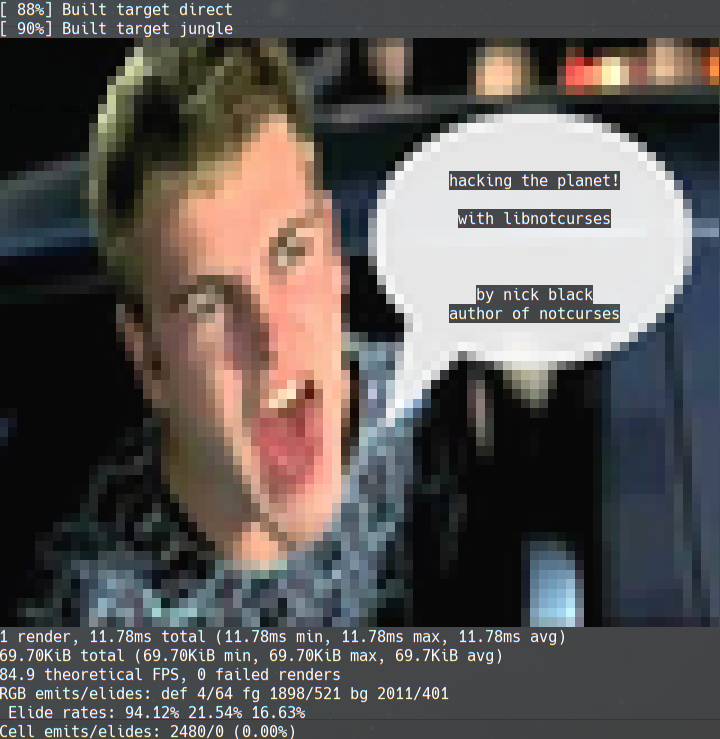
\includegraphics[width=.75\linewidth]{htp-with-notcurses.png}
\end{center}
\thispagestyle{empty}
%%%%%%%%%%%%%%%%%%%%%%%%%%%%%%%%%%%%%%%%%%%%%%%%%%%%%%%%%%%%%%%%%%%%%%%%

\clearpage
\pagenumbering{roman}

%%%%%%%%%%%%%%%%%%%%%%%%%%%%%%%%%%%%%%%%%%%%%%%%%%%%%%%%%%%%%%%%%%%%%%%%
\vspace*{1.25in}
\begin{figure}[!htbp]
\centering
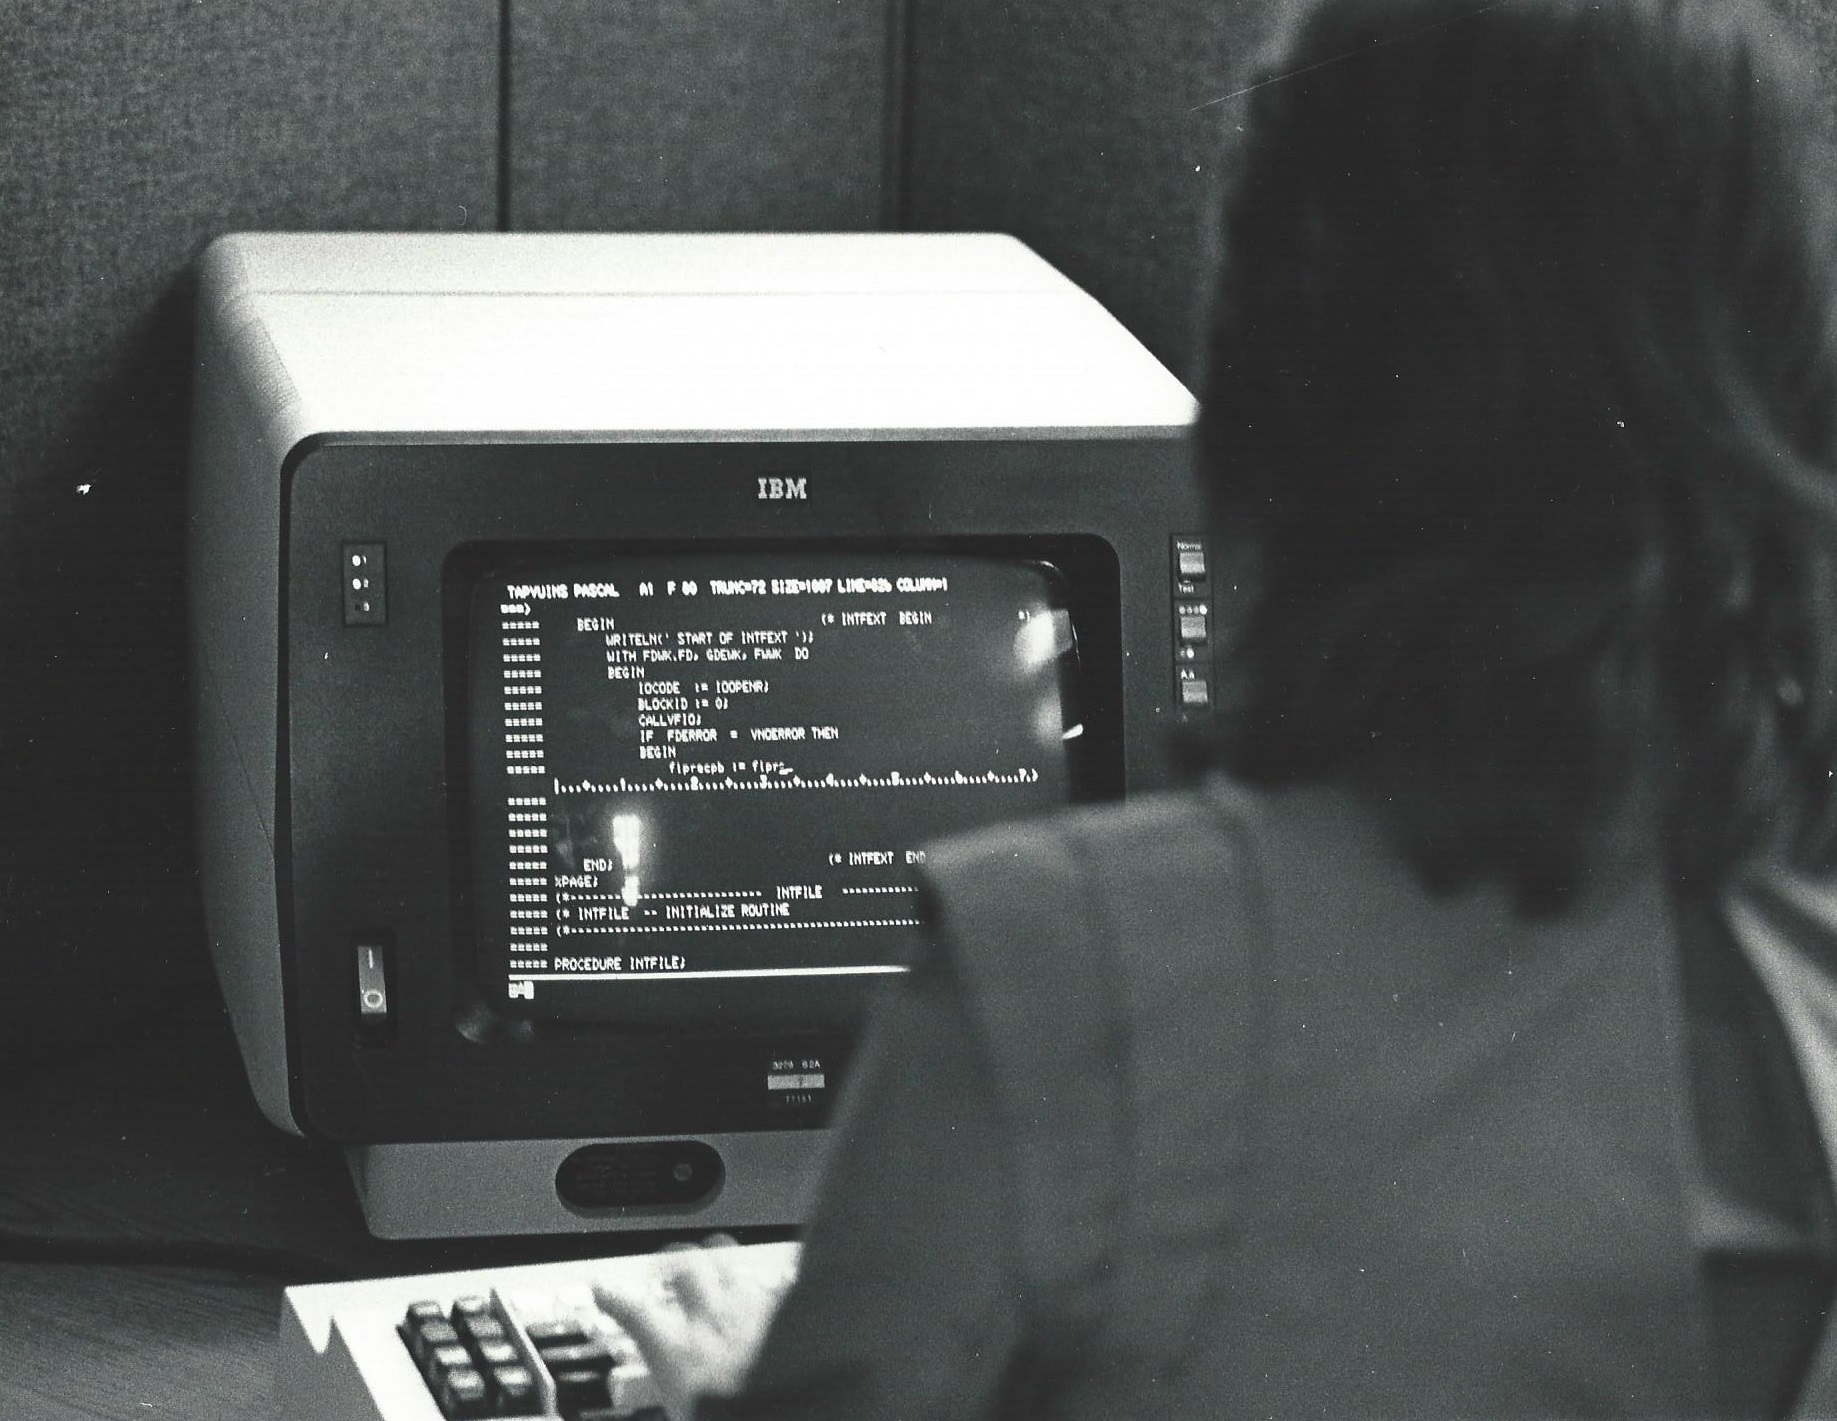
\includegraphics[width=1\linewidth]{media/ibm3270.jpg}
\caption[A programmer at her IBM 3270]{A programmer at her IBM 3270 2A. \textit{Source: Jonathan Schilling}.}
\end{figure}
\clearpage
\vspace*{1in}
\begin{center}
  \textit{For T.\ S.\ Eliot, il miglior fabbro.} \\
  \vspace{.25in}
  \textit{For Jeanette Martin, for exhortations to go H.A.M. \\
  \vspace{.25in}
  For Jim Greenlee, for speaking rigor to my programming.\\
  \vspace{.25in}
    For Prof.\ Hyesoon Kim, for introducing me to the glorious world
    inside the die.\\
  \vspace{.25in}
    For Prof.\ Richard Vuduc, for demonstrating serenity in brilliance, and kindness in dominance.\\}
  \vspace{1in}\ldots but mostly for Emily.
\end{center}
\clearpage
%%%%%%%%%%%%%%%%%%%%%%%%%%%%%%%%%%%%%%%%%%%%%%%%%%%%%%%%%%%%%%%%%%%%%%%%

\tableofcontents
\vfill
\begin{center}
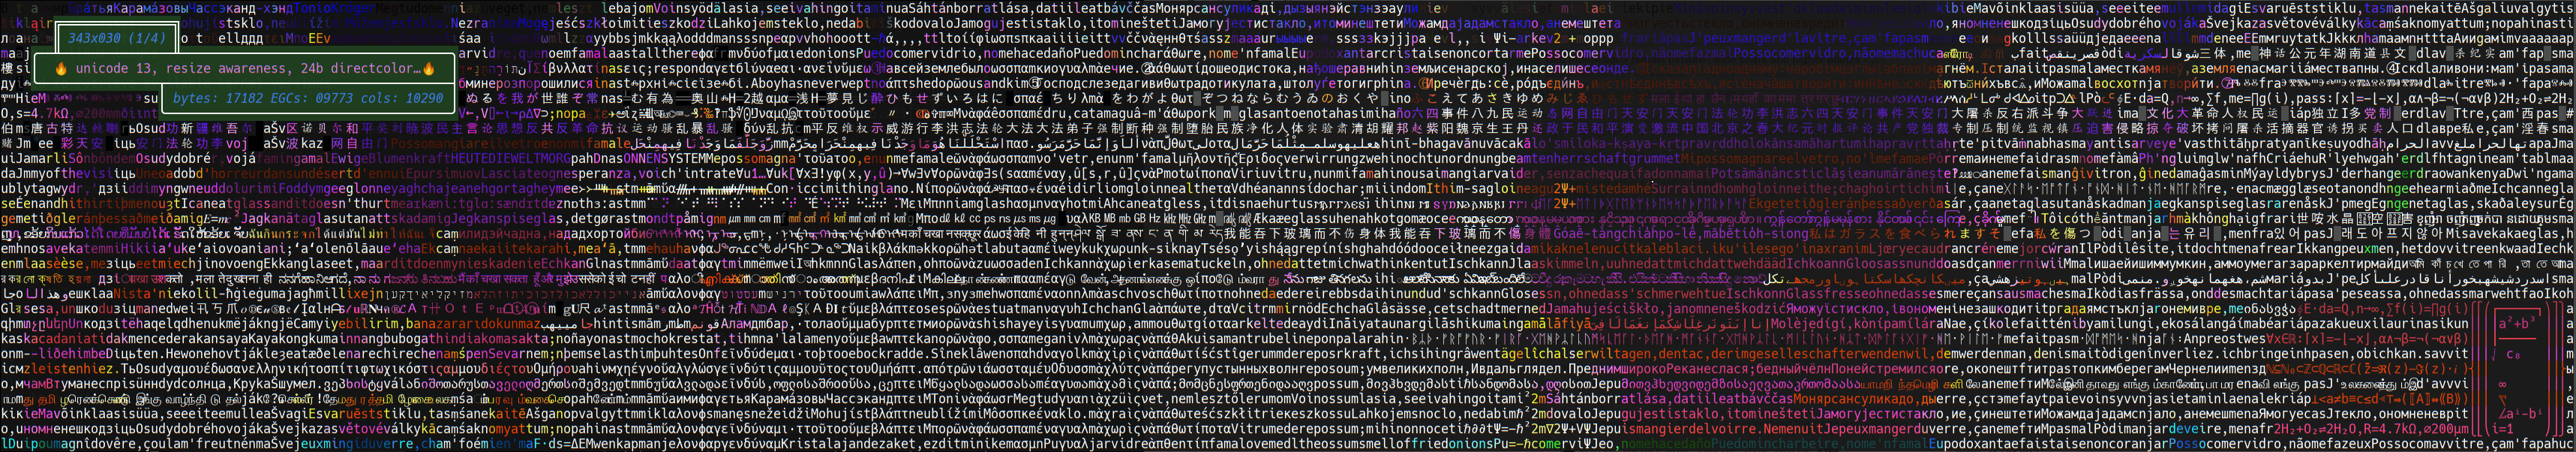
\includegraphics[width=1\linewidth]{media/widechars.png}
\end{center}

\cleardoublepage
\phantomsection
\addcontentsline{toc}{section}{\listfigurename}
\listoffigures
\addcontentsline{toc}{section}{List of Listings}
\listoflistings
\addcontentsline{toc}{section}{\listtablename}
\listoftables
\clearpage
%%%%%%%%%%%%%%%%%%%%%%%%%%%%%%%%%%%%%%%%%%%%%%%%%%%%%%%%%%%%%%%%%%%%%%%%

\newpage
%%%%%%%%%%%%%%%%%%%%%%%%%%%%%%%%%%%%%%%%%%%%%%%%%%%%%%%%%%%%%%%%%%%%%%%%
\section{Foreward}
Hacking the Planet with Notcurses:\\
A Guide to Character Graphics and TUIs.

Copyright © 2020 Nick Black.

ISBN: 9798620069491

This edition corresponds to version 1.2.3 of the Notcurses
library, released 2020-03-07.

Notcurses can be downloaded from
\url{https://github.com/dankamongmen/notcurses}.

This document can be downloaded
from~\url{https://nick-black.com/htp-notcurses.pdf}.

Licensed under the Apache License, Version 2.0 (the ``License''); you may not
use this document except in compliance with the License. You may obtain a copy
of the License at \url{http://www.apache.org/licenses/LICENSE-2.0}.

Unless required by applicable law or agreed to in writing, software
distributed under the License is distributed on an ``AS IS'' BASIS,
WITHOUT WARRANTIES OR CONDITIONS OF ANY KIND, either express or implied.
See the License for the specific language governing permissions and
limitations under the License.

The entirety of this work is Free Documentation, written for love and released
to instruct. You should not have been charged to download this document. If
you'd like to show thanks for my efforts, I encourage a donation to
the~\href{https://www.thefire.org/}{Foundation for Individual Rights in Education} (\url{https://www.thefire.org/}).

This work was prepared on a Debian Unstable workstation and an Arch Linux laptop,
using Vim, \XeLaTeX, and the GIMP.

Tetris © The Tetris Company, LLC.
\textit{Hackers (1995)} © United Artists Pictures.
\textit{House of Leaves (2000)} © Penguin Random House.
``Ruins with Rain'' © Mark Ferrari/Living Worlds.
``Final Fantasy'' © Square Enix Co Ltd.
``Super Mario Bros.'' © Nintendo of America.
``Ninja Gaiden'' © Koei Tecmo America.
``Street Fighter II'' and ``Mega Man 2'' © Capcom of America.
Please don't sue me.

\subsection{¡Peligro!}

The code written for this book attempts to minimize use of vertical space
without eliding error checking (or crossing into the realms of the grotesque).
Error handling is a fundamental slog of C programming, one that
inevitably complicates reliable applications.

These listings cannot be considered examples of good general style\ldots but they \textit{do} get the job done.

Three irregular idioms show up frequently:

\begin{denseitemize}
\item{Use of |= to collect non-zero return values from each of a series of
      non-interdependent function calls.}
\item{Right-hand-side conditionals fed into |=, e.g. \texttt{r |= (printf("dank") < 0);}.}
\item{Extensive use of ||'s short-circuiting property.}
\end{denseitemize}

\clearpage
%%%%%%%%%%%%%%%%%%%%%%%%%%%%%%%%%%%%%%%%%%%%%%%%%%%%%%%%%%%%%%%%%%%%%%%%
\pagenumbering{arabic}

\epigraph{Our fine arts were developed, their types and uses were established, in times
very different from the present, by men whose power of action upon things was
insignificant in comparison with ours. But the amazing growth of our
techniques, the adaptability and precision they have attained, the ideas and
habits they are creating, make it a certainty that profound changes are
impending in the ancient craft of the Beautiful.}{Paul Valéry}
\section{Introduction}

I implemented Notcurses in the winter of 2019 after having a few patches
rejected from NCURSES. The first commit was pushed 2019-11-16. It proved to
be seductive as hell, and it was only with difficulty that I tore myself away
following three months of hard work. I started writing this manuscript
2020-02-12, following the 1.1.8 release. By that time, Notcurses subsumed large
chunks of NCURSES, adding a great deal more. The project had three major goals:

\begin{denseitemize}
\item to provide NCURSES-like functionality with 24-bit color, safety in the
    presence of multithreading, and full Unicode support,
\item to reduce the amount of boilerplate code necessary for the UIs of my
    TUI applications, including \textit{growlight} and \textit{omphalos}, and
\item to portably facilitate the most vivid character graphics possible.
\end{denseitemize}

Many people asked how such a thing was useful. My usual response was that
numerous devices don't present a bitmap interface, that X11 GUIs run remotely
over SSH are effectively unusable, that plenty of machines don't have a GUI
environment installed, that there are obvious applications for large outdoor
displays, and that Sixel isn't well-supported across different
terminal emulators. It seems impossible in an age of gigatransistor graphics
cards, but the text environment still presents perceivably less latency
than most GUI toolkits. That I was able to remove thousands of lines
of NCURSES code from my applications was a nice side benefit.

In truth, the main reasons were that it was fun, and I wanted to see how far
I could push it.

As I write this, Notcurses is present in Arch's AUR, and is awaiting promotion
from the Debian Incoming queue. Written as a C core, it enjoys \CC, Python, and
Rust wrappers. I have submitted it as a backend to NEStopia and RetroArch, and
intend to integrate it into Mesa as an OpenGL backend. So long as one can live
with the limited resolution available when a screen is divided into rectangular
cells, it can handle any graphics thrown at it. I hope to see it displace
NCURSES as the go-to character graphics library for new applications (there is
little value in porting existing applications to Notcurses, since an unchanged
application wouldn't take advantage of its advanced features).

While the X/Open Curses specification is unlikely to ever go away (nor should
it, as a lowest-common-denominator interface to devices Notcurses is unlikely
to ever support), I believe Notcurses to present a superior and
implementation for modern TUI applications.

The console ain't dead! Hack on, hax0rs.

\vfill

\begin{flushright}
  \textit{---February 2020, Atlanta}
\end{flushright}

\newpage
%%%%%%%%%%%%%%%%%%%%%%%%%%%%%%%%%%%%%%%%%%%%%%%%%%%%%%%%%%%%%%%%%%%%%%%%

\vfill
\begin{figure}
\centering
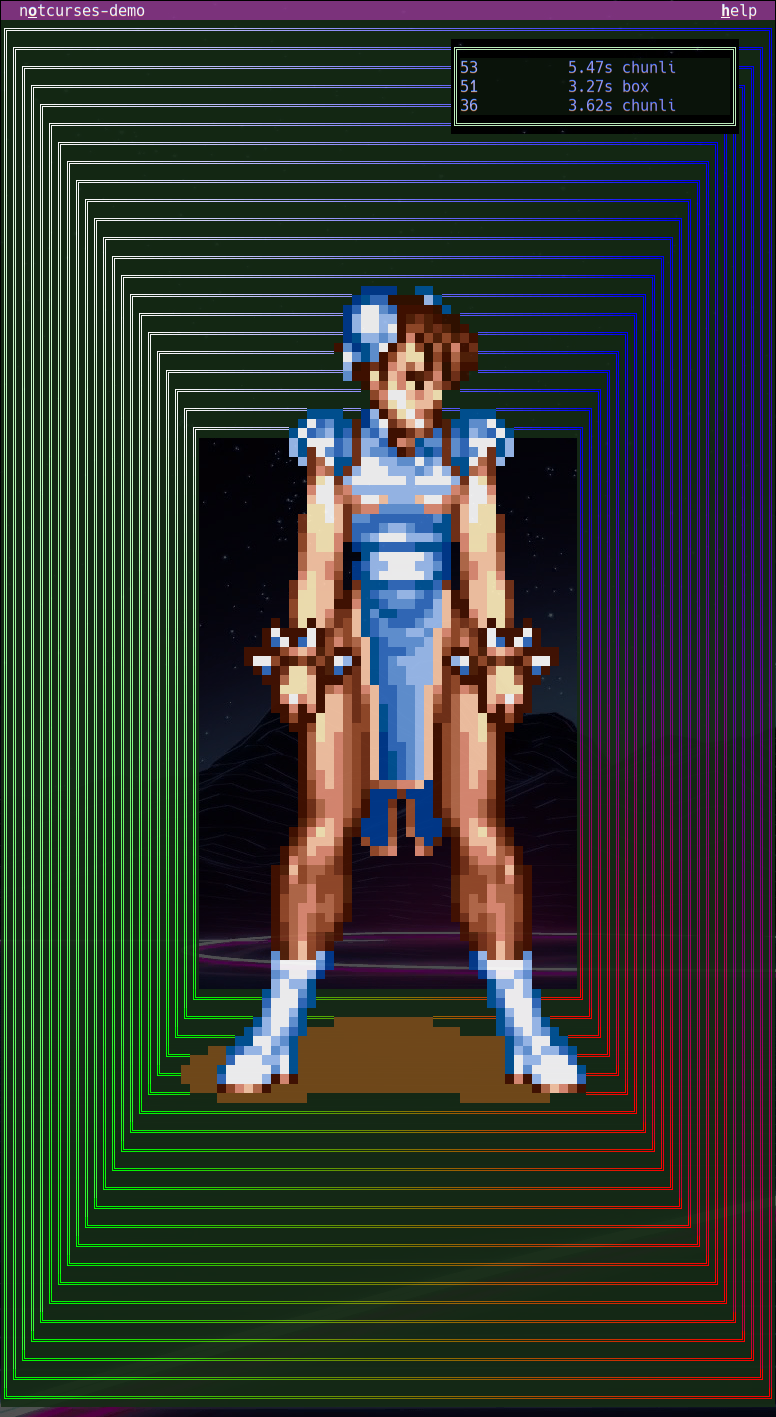
\includegraphics[width=.65\linewidth]{media/chunli-box-front.png}
\caption[An example render.]{A rendered scene from the ``chunli'' demo (see Chapter~\ref{sec:ncdemo}),
  using some of the advanced capabilities of Notcurses. The Chun-Li sprite has
  been loaded from a transparent PNG (Chapter~\ref{sec:libav}) atop boxes
  (Chapter~\ref{sec:boxes} drawn using Unicode (Chapter~\ref{section:unicode})
  and linear interpolations (Chapter~\ref{sec:lerps}). Along the top is a
  menu (Chapter~\ref{sec:menus}) and an independent plane (Chapter~\ref{sec:planes});
  both can be controlled with mice (Chapter~\ref{sec:input}). In the center,
  the desktop can be seen through the transparent background of the terminal.}
\end{figure}
\vfill
\newpage

\section{Right, what's all this, then?}
\label{sec:start}
\epigraph{A terminal is at the end of an electric wire, a shell is the home of a turtle, tty is a strange abbreviation and a console is a kind of cabinet.}{Gilles Leblanc\cite{gillesSO}}
Character graphics, aka text mode, aka the display side of a terminal, is
visualization that works with fonts rather than a pixel framebuffer\footnote{``Contones'', as raster graphics are known to printers.}
or a vector canvas\footnote{Nothing keeps you from implementing character graphics
with pixels or vectors, of course.}. There is furthermore an expectation that
this font is a fixed-width one---that all rendered glyphs are integer multiples
of some narrowest non-trivial glyph.

Given the same display hardware,

\begin{denseitemize}
\item{Character graphics are usually strictly less powerful than pure raster graphics, and}
\item{their lower effective resolution typically implies lower bandwidth requirements.}
\end{denseitemize}

A TUI (text user interface) is a holistic model, view, and controller implemented
using character graphics. TUIs, like WIMP\footnote{Windows, icons, menus, pointers, a paradigm so pervasive that
the industry collectively treasures a Wiemarian\cite{thirdreich} memory of Xerox PARC's noble
engineers stabbed in the back by management (not unlike the Oatmeal-fostered\cite{fuckoatmeal}
myopia regarding Edison and Tesla. I'll take Thomas Alva over Matthew Inman any
day). It too often goes unmentioned that the Alto and Star were as unusable as they were visionary\cite{lightningdealers}.
This is of course still superior to Java, which isn't even visionary.} GUIs,
freely move the cursor around their rectilinear display, as opposed to
line-oriented CLIs and their ineluctable marches through the scrolling region.

Given the same interactive task,\footnote{These relations are not
fundamental, but emerge from the grim meathook realities of GUI toolkits.}

\begin{denseitemize}
\item{A TUI implementation is almost certainly a smaller memory and disk footprint than a GUI,}
\item{a good TUI implementation might introduce less latency, and}
\item{a properly-done TUI implementation can often be significantly more portable.}
\end{denseitemize}

Of course, it can also be a big pile of character graphics shit.

For over two decades, NCURSES (a free software implementation of the X/Open Curses\cite{cursesosi}
specification, plus extensions\cite{ncursesfaq}) has been a ubiquitous go-to for implementing
TUIs. Maintainter (and author, in large part) Thomas E.\ Dickey
exemplifies conservative and fastidious stewardship. Perfectly lovely TUIs can
be built using NCURSES (as seen in Figure~\ref{fig:ncurses-tuis}), but it \textit{does}
have its origins in the 8-bit era, and shows its age.

\begin{figure}[!hbtp]
  \centering
    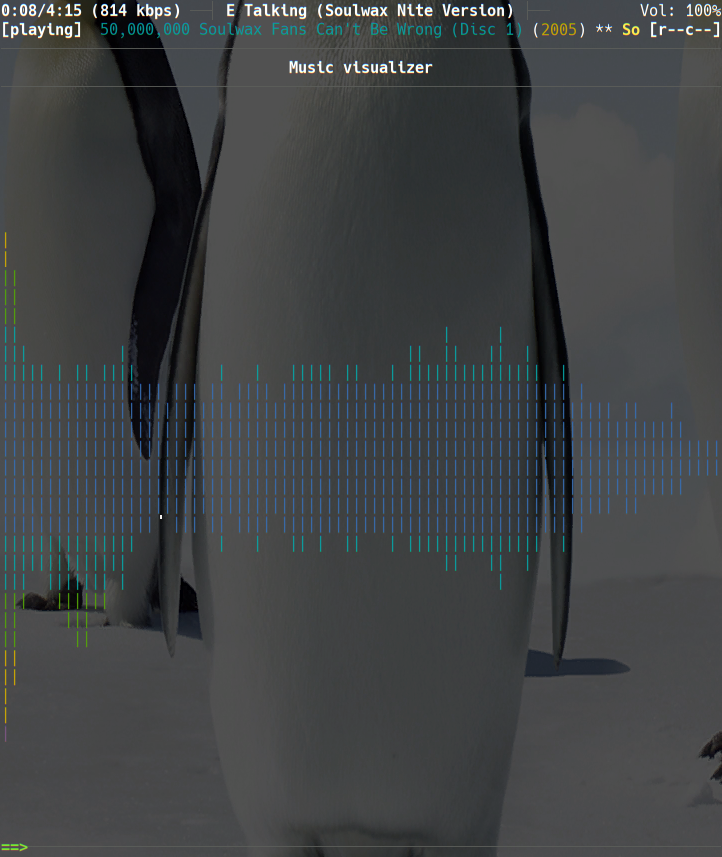
\includegraphics[width=.4\linewidth]{media/tui-ncmpcpp.png}
    \hfill
    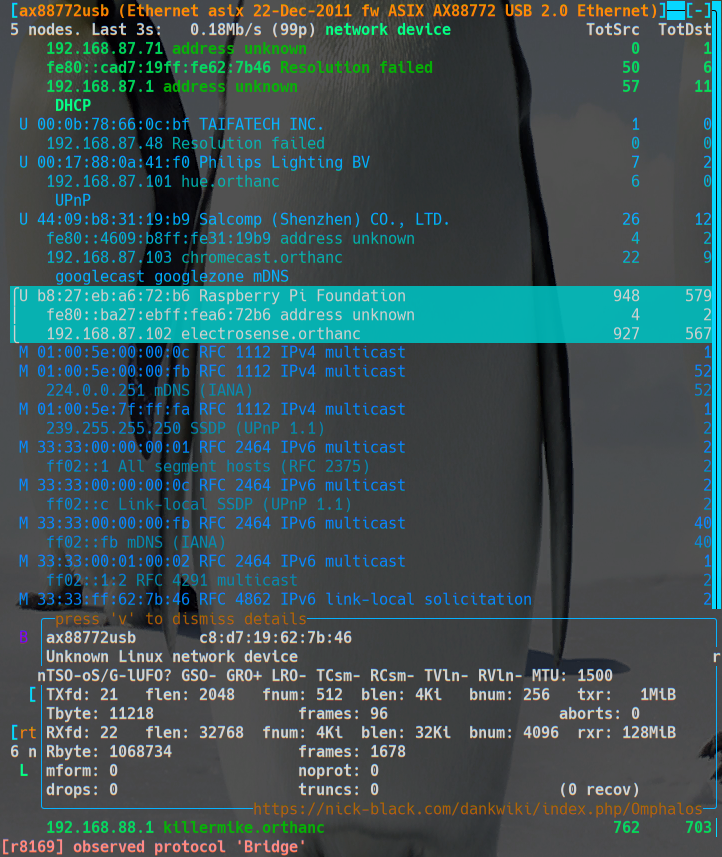
\includegraphics[width=.4\linewidth]{media/tui-omphalos.png}
    \caption[NCURSES TUIs: Ncmpcpp and Omphalos.]
    {\texttt{ncmpcpp}, a \CC application
      that has driven my Music Player Daemon since 2008 or so.
      \texttt{omphalos}, a C application
      written using NCURSES in its extended mode.}
  \label{fig:ncurses-tuis}
\end{figure}

\begin{figure}[!htbp] \centering
    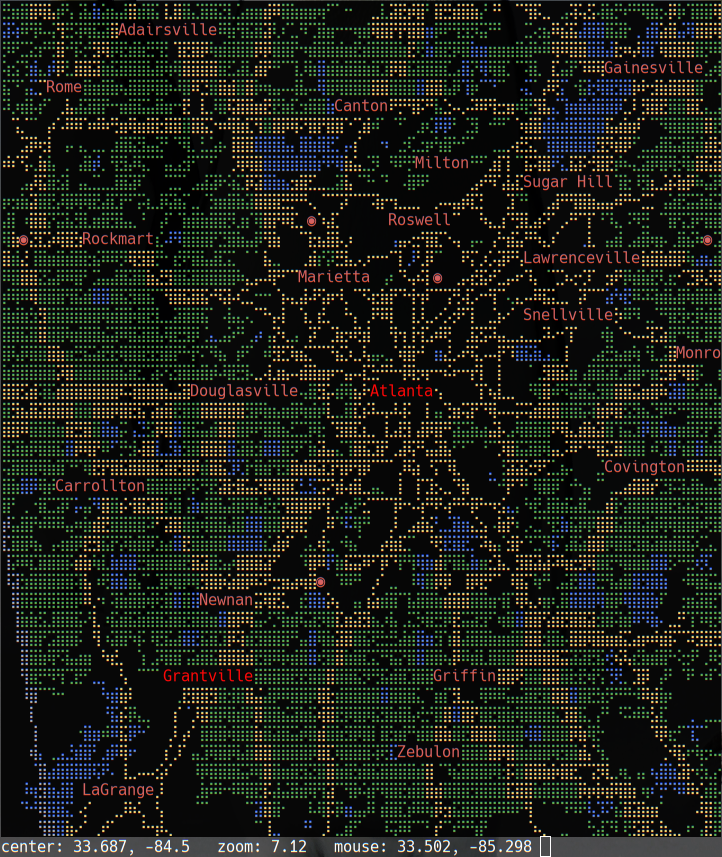
\includegraphics[width=.4\linewidth]{media/tui-mapscii.png}
    \hfill
    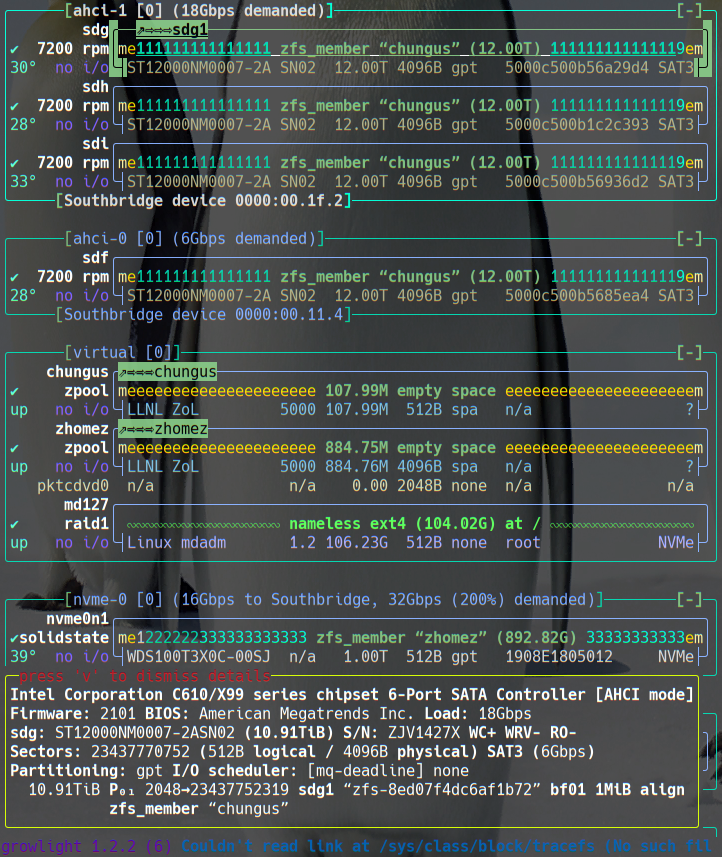
\includegraphics[width=.4\linewidth]{media/tui-growlight.png}
    \caption[Non-NCURSES TUIs: Mapscii and Growlight.]{\texttt{mapscii}, a
    node.js application, blew my mind when I first saw it. The high resolution
    is achieved by using Braille characters, trading away some color control.
    \texttt{growlight} began life as an NCURSES C program, but was ported to
    Notcurses in 2019.}
  \label{fig:notncurses-tuis}
\end{figure}

Implementing a TUI will usually require, at a minimum:
\begin{denseitemize}
\item{Receiving input from user devices, including keyboards and mice,}
\item{some manner of user configuration widgets (menus, etc.),}
\item{watching for some other event(s) from the system, and},
\item{juggling these various components without wastefully polling, nor
       introducing undue latency, and enforcing safe synchronized access to
       the graphics interface.}
\end{denseitemize}

Perhaps most terrifyingly, it will require user interface design. Notcurses
attempts to assist with this by providing numerous ready-made widgets.

This text has two goals:
\begin{denseitemize}
\item{To provide a firm footing for design and implementation of character
    graphics and TUIs, elucidating the dimensions of design, along with difficulties
    to avoid, and}
\item{to serve as ``narrative reference''\cite{newjournalism} for my Notcurses
      library, and as a starting place for newcomers.}
\end{denseitemize}

\begin{figure}[!htbp]
\centering 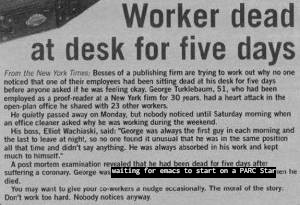
\includegraphics[width=.5\linewidth]{media/emacs-xerox.jpg}
  \caption{Put not your trust in hackers making a fetish of Xerox PARC.}
  \label{fig:xeroxemacs}
\end{figure}

Cell graphics are primarily the realm of \textit{terminals}, which for the
purposes of this book encompass any means by which input devices act to drive
some process generating glyph-based output to a display. This includes hardware
terminals (inputs integrated with displays, connected to a computer as a unit),
operating system consoles (text-mode interfaces operating with the graphics
engine directly connected to the terminal driver), terminal multiplexers (tools
like \texttt{screen}, \texttt{tmux}, and \texttt{mosh}, providing a
memory-persistent virtual terminal with which other terminals can interact),
and terminal emulators (applications which present a virtual terminal atop the
shared input and raster output methods of a graphical user environment).
There's some vagueness and variety involved with these terms.

At its heart, a terminal is a line discipline plus two buffers: an input buffer
to collect user-generated events (possibly from multiple devices), and an
output buffer to be processed and displayed. The buffers can be modeled as byte
streams, mutating the output at the time of their display (in contrast to e.g.\
a framebuffer, where the entirety of the screen is present at any given time).
The earliest terminals were electromechanical teletypes, reproducing their
input as line-based print on paper. These gave rise to ``dumb terminals''
(cathode-ray displays with a scrolling rectilinear output area). ``Smart
terminals'' followed, with the ability to move freely within their display
area, and also to extract and act upon ``control codes'' embedded in the output
stream. The text modes of the first video cards were designed around the
capabilities of these smart terminals. This brings us to the present, wherein
high-powered LED displays have their pixels summoned up and ordered into
formations suitable for the reconstruction of 1970s technology (a history of
terminals is presented in Appendix~\ref{sec:terminals}).

The machine on which I'm preparing this \LaTeX\ contains a
TU104 GPU consisting of over thirteen billion 12nm-process transistors,
rendering its output to a 3440x1440 (almost five megapixel) display. Deep
within its silicon heart remains a VGA 80x25 text mode engine\cite{vga}, inherited
largely unchanged from the EGA, the CGA, the IBM Monochrome Display Adapter\footnote{The
history of video display standards since 1981's MDA is a story of imprecision,
dashed hopes, and idle dreams. Good luck finding authoritative references
for anything beyond \texttt{int 10h} real mode operation prior to version 1.0
of the SuperVGA VESA BIOS Extension\cite{videostandards}, released 1989-10-01\cite{vesa}.},
and before that smart terminals\footnote{As early as 1971, the block-oriented
IBM 3277 Model 2 ``green screen'' shipped with 80x24.}.


I mainly use this modern marvel to drive terminal emulators of 80 columns.

\newpage
%%%%%%%%%%%%%%%%%%%%%%%%%%%%%%%%%%%%%%%%%%%%%%%%%%%%%%%%%%%%%%%%%%%%%%%%

\section{Using direct mode with standard I\/O}
\label{sec:direct}
\epigraph{Unscrew the locks from the doors!\\Unscrew the doors themselves from their jambs!}{Walt Whitman, \textit{Song of Myself}}
Many tools don't intend to be full-screen TUI applications, but instead
implement that purest of UNIX interfaces: newline-delimited text, oblivious
to screen geometry, capable of being fed as input to other, similar programs.
For such tools, the full Notcurses capabilities are neither necessary nor
desirable. These programs are typically non-interactive: humans might peruse
their outputs and prepare their inputs, but they effectively run as a batch
task.

 Such tools might still want to colorize and otherwise style their output, at
least when being output to a terminal. This can be accomplished using the
\texttt{ncdirect} subset of Notcurses, and is known as \textit{direct mode}. Direct
mode functionality should not usually be mixed with other Notcurses calls.
Unlike full Notcurses, there is no explicit rendering step in direct mode, and
it is intended to be mixed among other use of standard I/O. Essentially, direct
mode ``styles your \texttt{printf()}s.'' Similarly to full Notcurses, direct mode
requires a valid and correct terminfo database entry, supplied via either the
\texttt{termtype} parameter to \texttt{ncdirect\_init()} or the \texttt{TERM} environment
variable. It does \textit{not}, however, require any particular encoding or
other locale properties\cite{setlocale} (full Notcurses requires a
properly-configured ASCII or UTF-8 locale).

Enter direct mode via a call to \texttt{ncdirect\_init()} with a successful
return of a non-\texttt{NULL} pointer to \texttt{struct ncdirect}. It is
typical to invoke this function as \texttt{ncdirect\_init(NULL, stdout)}. In this case, the terminal type must be present in the
\texttt{TERM} environment variable (this should have been done by the
terminal). The buffering and blocking status of \texttt{fp} will not be
changed. \texttt{NULL} is returned for any number of possible errors.
Otherwise, the \texttt{struct ncdirect} is ready to go, and should be cleaned
up with \texttt{ncdirect\_stop()}.

\begin{listing}[!htbp]
\begin{minted}{C}
// Initialize a direct-mode notcurses context on the connected terminal at 'fp'. 'fp' must be a tty. You'll usually
// want stdout. Direct mode supportes a limited subset of notcurses routines which directly affect 'fp', and neither
// supports nor requires notcurses_render(). This can be used to add color and styling to text in the standard
// output paradigm. Returns NULL on error, including any failure initializing terminfo.
struct ncdirect* ncdirect_init(const char* termtype, FILE* fp);

// Release 'nc' and any associated resources. 0 on success, non-0 on failure.
int ncdirect_stop(struct ncdirect* nc);
\end{minted}
\caption{Initializing and stopping directmode.}
\end{listing}

Between these two calls, inject stylizing control codes into the \texttt{FILE*} with
the \texttt{ncdirect} (the \texttt{stylebits} values are detailed in Chapter~\ref{sec:attribute}).
As detailed in Chapter~\ref{sec:channels}, the terminal has a ``default foreground color''
and ``default background color''. Return to these default colors with
\texttt{ncdirect\_fg\_default()} and \texttt{ncdirect\_bg\_default()}.

\begin{listing}[!htbp]
\begin{minted}{C}
int ncdirect_bg_rgb8(struct ncdirect* n, unsigned r, unsigned g, unsigned b);
int ncdirect_fg_rgb8(struct ncdirect* n, unsigned r, unsigned g, unsigned b);
int ncdirect_fg(struct ncdirect* n, unsigned rgb);
int ncdirect_bg(struct ncdirect* n, unsigned rgb);
int ncdirect_styles_set(struct ncdirect* n, unsigned stylebits);
int ncdirect_styles_on(struct ncdirect* n, unsigned stylebits);
int ncdirect_styles_off(struct ncdirect* n, unsigned stylebits);
int ncdirect_clear(struct ncdirect* n);
int ncdirect_fg_default(struct ncdirect* n);
int ncdirect_bg_default(struct ncdirect* n);
\end{minted}
\caption{The \texttt{ncdirect} styling API.}
\end{listing}

Direct mode allows the cursor to be moved in two-dimensional space, and
provides helpers for determining the terminal geometry. Either \texttt{y} or
\texttt{x} may be specified as -1 to maintain location on the associated axis.

\begin{listing}[!htbp]
\begin{minted}{C}
int ncdirect_dim_x(const struct ncdirect* nc);
int ncdirect_dim_y(const struct ncdirect* nc);
int ncdirect_cursor_move_yx(struct ncdirect* n, int y, int x);
\end{minted}
\caption{Cursor management with \texttt{ncdirect}.}
\end{listing}

\subsection{Example: presenting \textit{\textcolor{blue}{House} of Leaves}}
Mark Z. Danielewski's experimental 2000 novel \textit{\textcolor{blue}{House} of Leaves}\cite{danielewski2000house} prints each
instance of the word \textcolor{blue}{house} in blue, even when it is a subword:

\begin{figure}[!htbp]
\centering 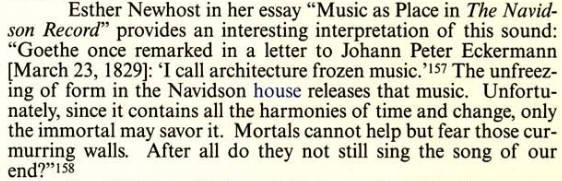
\includegraphics[width=.5\linewidth]{house-blue.png}
\caption{An excerpt from page 123 of \textit{\textcolor{blue}{House} of Leaves}.}
\label{fig:houseofleaves}
\end{figure}

We can easily write code to reproduce this effect for standard input and output.
Listing~\ref{list:holformatter} works as expected (see
Figure~\ref{fig:houseout}), but there are a few things worth noting about its
code. First, observe how much of the logic is devoted to checking and
propagating errors! Perhaps contrary to common expectation, reliable
code---especially when that code's primary effect is to write to
stdout---generally needs to check the results of e.g. \texttt{printf()} (what
happens if we're redirected to a file, and the disk is full?). A language
making use of exceptions would reduce if not eliminate this nonsense.

\begin{listing}[!htbp]
\inputminted[]{C}{code/hol-formatter.c}
\caption{\texttt{hol-formatter.c}, a streaming formatter.}
\label{list:holformatter}
\end{listing}

\begin{figure}[!htbp]
\centering 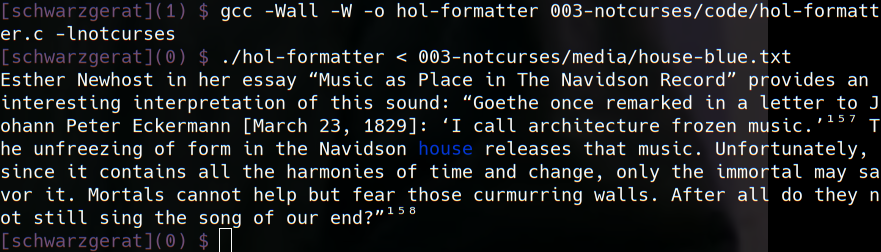
\includegraphics[width=.75\linewidth]{hol-formatted.png}
\caption[\texttt{hol-formatter} as run on OCRd input.]{\texttt{hol-formatter} as run on our input. We use \texttt{tesseract} for OCR, with solid results.}
\label{fig:houseout}
\end{figure}

So long as we're dealing with either ASCII or UTF-8 input, our simple, old-skool
\texttt{tolower(3)} is satisfactory \textit{for this problem}. The key
observation is that UTF-8 encoded text can be compared for equality by
a structure-oblivious~\texttt{memcmp(3)}, as of course can ASCII.
Unless we need to color e.g.~\textcolor{blue}{\texttt{ℏöûⓈᴇ}} (maybe we should,
maybe we shouldn't) this is safe, simple, and sufficient. If we \textit{do}
wish to collapse distinct but by some measure similar EGCs, we should normalize
input as prescribed by Unicode Standard Annex \#15\cite{annex15}.

We don't switch from blue to some other specified color, because we don't know
the background color of the terminal. Some people, possibly aliens, don't favor
a dark terminal background. If the terminal background were white, and we had
just used e.g. \texttt{ncdirect\_fg(n, 0xffffff)}, text following
``\textcolor{blue}{house}'' would be invisible.

One might observe that a user with a blue background will have invisible
``\textcolor{blue}{house}'' text. This is a real issue, one lacking a perfect
solution\footnote{Applying \texttt{NCSTYLE\_STANDOUT} might or might not help.}.
It is not generally possible to discover the RGB values of the default colors.
I suppose all one can do is rest easy, serene in the belief that white
backgrounds are one thing, but people with chromatic backgrounds deserve
whatever happens to them.

\subsection{Example: colorizing a dumb game}
Imagine we've written the simple guessing game in Listing~\ref{list:guessgame}.

\begin{listing}[!htbp]
\inputminted[]{C}{code/hilostdio.c}
\caption{\texttt{hilostdio.c}, a simple guessing game.}
\label{list:guessgame}
\end{listing}

The correct approach for a player is binary search, and for an $N$-bit
\texttt{long}, we expect to guess the number in no more than $N$ tries. Let's
color the output to indicate how bad of a guess was offered. We'll use red for
low guesses, blue for high guesses, and break the 256 shades of each (assuming
the other two components to be fixed) uniformly across the $N$ levels of
logarithmic distance\footnote{This would be a good place to employ \gls{gamma correction}.}.
If we wanted to do this (see Listing~\ref{list:hilodirect}) without direct use of RGB color,
we'd either need accept fewer shades, or be forced to reprogram the palette.

\begin{listing}[!htbp]
\inputminted[]{C}{code/hilodirect.c}
\caption{\texttt{hilodirect.c}, a colorized version of the guessing game.}
\label{list:hilodirect}
\end{listing}

Stepping through the orders of magnitude\footnote{\texttt{\_\_builtin\_clzl()}
is a compiler intrinsic for \textit{count leading zeroes}. Exhaustive methods
for fast clzl can be found in \cite{hackerdelight}. Demonstrating that
absolute value of the difference of leading zeroes is a $lg_{2}$ difference
is left as an exercise for the reader.}, we get the expected gradient
(Figure~\ref{fig:colorguess}). Were we to actually play, the response would
converge to a balanced, strong green as we approached the correct answer.

\begin{figure}[!htbp]
\centering 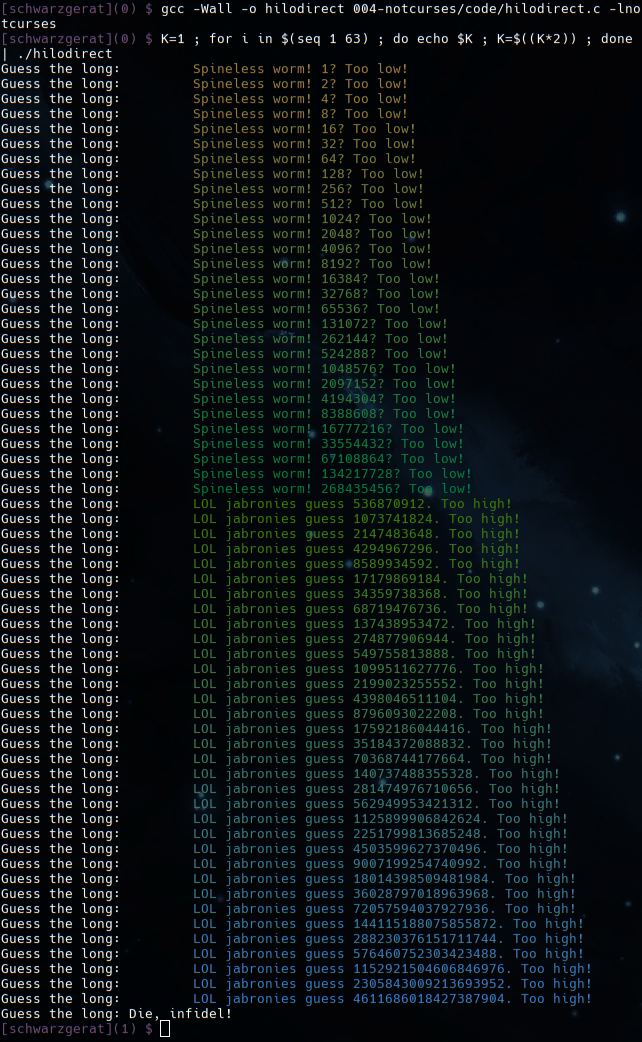
\includegraphics[width=.75\linewidth]{media/hilodirect.png}
\caption{Colorized output from~\texttt{hilodirect.c}.}
\label{fig:colorguess}
\end{figure}

\subsection{Advanced coëxistence with stdio}
It is most common to initialize Notcurses with \texttt{stdout}, whether in
direct mode or fullscreen mode. This isn't the only way to operate, though.
By opening the tty directly using \texttt{/dev/tty}\cite{tty4}, and providing
this \texttt{FILE*} to Notcurses, a program passing its standard output to
another process can make concurrent use of Notcurses on the display, in either
direct or fullscreen mode. This is how the \texttt{notcurses-pipe} program
works\footnote{See \url{https://github.com/dankamongmen/notcurses/issues/381}.}.

For programs that need to write to the terminal, but want to ``overlay'' some
Notcurses, fullscreen mode won't work (though the program could be run in an
\texttt{ncprocess} widget; see Chapter~\ref{sec:uiwidgets}). Direct mode, however, is
a possibility. I've not yet written the example\footnote{Send me patches! Or
I'll do it\ldots eventually \url{https://github.com/dankamongmen/notcurses/issues/382}.}, but it is possible to, for
instance, periodically acquire the current cursor position, move elsewhere on
the screen, update a HUD, and return to the departure position. Scrolling could
be addressed by retaining a copy of any obliterated output. This would suffer
a startup period of one screen, during which the area scrolled above the HUD
would be cleared. This could be avoided by aligning the HUD with the top of
the terminal.

\newpage

%%%%%%%%%%%%%%%%%%%%%%%%%%%%%%%%%%%%%%%%%%%%%%%%%%%%%%%%%%%%%%%%%%%%%%%%
\section{Using fullscreen mode}
\label{sec:fullscreen}
\epigraph{This is how space begins, with words only, signs traced on the blank page. To describe space: to name it, to trace it, like those portolano-makers who saturated the coastlines with the names of harbours, the names of capes, the names of inlets, until in the end the land was only separated from the sea by a continuous ribbon of text. Is the aleph, that place in Borges from which the entire world is visible simultaneously, anything other than an alphabet?}{Georges Perec, \textit{Species of Spaces}}
From this chapter forward, we will be using the fullscreen mode of Notcurses,
opening up all of its capabilities. This comes at a cost: while fullscreen mode
is being used, it is not safe to use standard I/O in conjunction with the
terminal controlled by Notcurses. Doing so is likely to (at a minimum) corrupt
the screen. If \texttt{stdout} and \texttt{stderr} are attached to the same
terminal (as they usually are in an interactive session), and \texttt{stdout}
is provided to Notcurses, output to \texttt{stderr} will corrupt the display
just as thoroughly as output to \texttt{stdout}. If your fullscreen Notcurses
program intends to log to \texttt{stderr}, you should first ensure that that
it has been redirected or is otherwise going somewhere different than
\texttt{stdout}. Note that simply rerendering the output will \textit{not}
necessarily clean up corruption, even following \texttt{ncplane\_erase()}
operations, since Notcurses optimizes its rendering based on its concept of the
screen. A call to \texttt{notcurses\_refresh()} will be necessary to sync the
the physical screen to Notcurses's concept thereof.

It is possible for the screen to be corrupted by external agents. For this
reason, Ctrl+L is by tradition bound to screen redrawing. You should hook this
input up to \texttt{notcurses\_refresh()} unless you have good reasons not to
do so (this is not default behavior of Notcurses only because Notcurses does
not itself read input). It is sadly not possible for such corruption to be
efficiently and generally detected.

It is possible for the attached terminal to be resized, especially (but not
only) for terminal emulators in GUI windowing environments\footnote{This could
also happen when refitting a \texttt{screen} or \texttt{tmux} session.
Even on the Linux or FreeBSD console, this can happen due to a change in video
resolution.}. Notcurses can detect such events, and synthesizes
\texttt{NCKEY\_RESIZE} inputs in response to them. If the screen shrinks, the
excess data relative to the constant origin will no longer be displayed (i.e.
the material in the upper left will be retained). If the screen is enlarged,
any data uncovered will be displayed, and the new area will otherwise be empty.
Some widgets can intelligently resize themselves in the face of screen
geometry changes (see Chapter~\ref{sec:uiwidgets}).

Notcurses prepares a given terminal for fullscreen mode in \texttt{notcurses\_init()}

\begin{listing}[!htbp]
\begin{minted}{C}
// Initialize a notcurses context on the connected terminal at 'fp'. 'fp' must
// be a tty. You'll usually want stdout. Returns NULL on error, including any
// failure initializing terminfo.
struct notcurses* notcurses_init(const notcurses_options* opts, FILE* fp);

// Destroy a notcurses instance, restoring the terminal to its original state.
int notcurses_stop(struct notcurses* nc);
\end{minted}
\caption{Initializing and stopping fullscreen mode.}
\end{listing}

Before calling \texttt{notcurses\_init()} (and usually as one of the first lines
of the program) it is necessary to set the current locale via the standard
library function \texttt{setlocale()}. A coverage of ANSI/ISO C locales is beyond
the scope of this text, but it is usually sufficient to call
\texttt{setlocale(LC\_ALL, "")}, relying on the user's configured \texttt{LANG}
environment variable. Notcurses only supports those locales using
US-ASCII or UTF-8 encodings (see Chapter~\ref{section:unicode} for more
information on character encodings), and its capabilities on US-ASCII
are \textit{severely} constrained. \texttt{notcurses\_init()} will return an
error for any other encoding (see Figure~\ref{fig:encodingfail}).

\begin{figure}[!htbp]
\centering 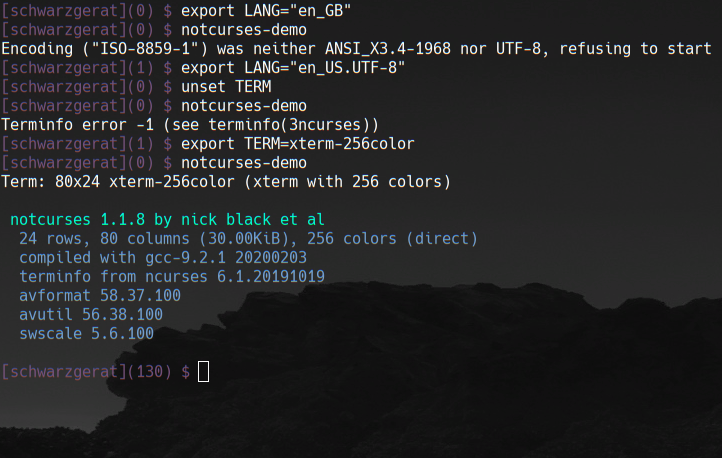
\includegraphics[width=.7\linewidth]{media/notcurses-init-fails.png}
\caption{Notcurses refusing to start due to an unsupported character encoding.}
\label{fig:encodingfail}
\end{figure}

By default (assuming the \texttt{enter\_ca\_mode} terminfo capability is expressed),
Notcurses attempts to enter the ``\gls{smcup}''. Using the alternate screen
implies:
\begin{denseitemize}
\item{The screen will be cleared upon entry,}
\item{Output will not be appended to the scrollback buffer, and}
\item{On exit, output will be cleared.}
\end{denseitemize}
Whether or not the original screen contents are restored is terminal-dependent
(if the \texttt{non\_rev\_rmcup} terminfo capability is defined, the original
contents will \textit{not} be restored). The alternate screen is generally
useful, but some users don't like it, so it's wise to expose this via a
configuration option. Disabling use of the alternate screen can be done via the
\texttt{notcurses\_options} field \texttt{inhibit\_alternate\_screen}.

Successful creation of a \texttt{struct notcurses} implies the existence of
a \texttt{struct ncplane}, the ``standard plane''\footnote{\texttt{ncplane}s,
discussed in depth in Chapter~\ref{ncplane}, are the fundamental drawing surfaces of Notcurses.}.
This standard plane cannot be destroyed without destroying the containing
Notcurses context, nor can it be moved or resized by the user. Its size always
matches Notcurses's concept of the terminal's screen size, and its origin
always corresponds precisely to the terminal's origin. Aside from these
restrictions, the standard plane is a drawable surface like any other
\texttt{ncplane}---it can be moved along the z-axis, written to with arbitrary
glyphs and styles, made transparent, etc.

Once you're done using a \texttt{struct notcurses}, it's important to destroy
it with \texttt{notcurses\_stop()}, even if your process exits abnormally. By
default, Notcurses registers signal handlers for most fatal signals. These
handlers will call \texttt{notcurses\_stop()} and then pass the signal to the
orginal actions. You can disable this with the \texttt{no\_quit\_sighandlers}
field of \texttt{notcurses\_options}, but there aren't very many good reasons
to do so.

\subsection{The \texttt{notcurses\_options} structure}
The first parameter to \texttt{notcurses\_init()} is a (possibly \texttt{NULL})
\texttt{notcurses\_options}. This structure has been defined such that the
default options are equivalent to a zero-initialized structure. Passing \texttt{NULL}
is thus equivalent to passing a zero-initialized \texttt{notcurses\_options}.
The fields therein include:
\begin{denseitemize}
\item{\texttt{const char* termtype}: The name of the terminfo database entry to
    use. If \texttt{NULL}, the value of the environment variable \texttt{TERM}
    is used. Failure to initialize the terminfo database will result in a
    \texttt{notcurses\_init()} failure.} A defined but invalid or suboptimal
    entry will result in garbage, missing output, poor performance, reduced
    colors, and unsightly weight gain.
\item{\texttt{bool inhibit\_alternate\_screen}: As noted above, this prevents
    Notcurses from making use of the alternate screen, even if the \texttt{enter\_ca\_mode}
    terminfo capability is defined. It's best to wire this up to a user-managed
    option. Not using the alternate screen can look weird upon return to the
    shell (see Figure~\ref{fig:altscreen}).

\begin{figure}[!htbp]
\centering 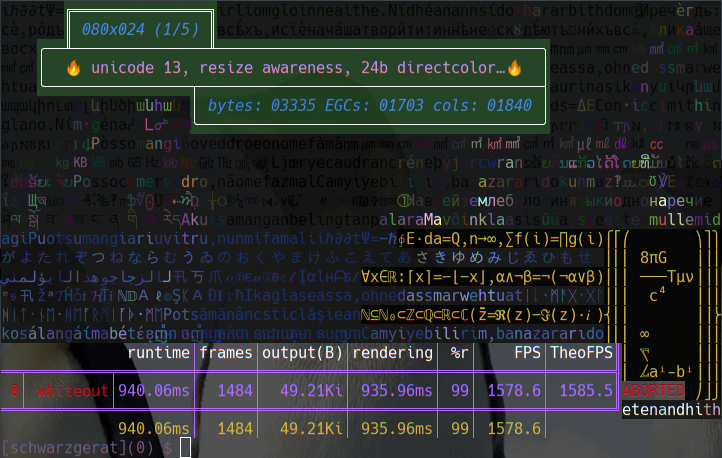
\includegraphics[width=.7\linewidth]{media/no-alternate-screen.png}
\caption[Inhibiting use of the alternate screen.]{\texttt{notcurses-demo} can be invoked with \texttt{-k} to avoid
  using the alternate screen. Here, we see its output left on the screen as
  we return to our shell.}
\label{fig:altscreen}
\end{figure}
  }
\item{\texttt{bool retain\_cursor}: Notcurses hides the cursor by default.
    Set this to keep the cursor visible (the cursor can be turned on and off
    at runtime with \texttt{notcurses\_cursor\_enable()} and
    \texttt{notcurses\_cursor\_disable()}).}
\item{\texttt{bool suppress\_banner}: At startup, Notcurses emits some
    diagnostics and/or warnings, including version information and details
    about the current terminal. At shutdown, it prints performance statistics.
    These outputs \textit{do not} go to the alternate screen. Set this
    field to disable these outputs, but be aware that doing so might hide
    important warnings (see Figure~\ref{fig:banner}).

    \begin{figure}[!htbp]
      \centering 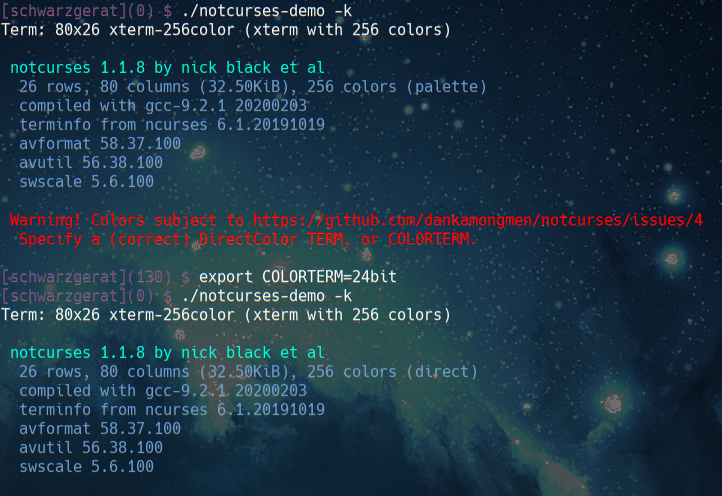
\includegraphics[width=.7\linewidth]{media/notcurses-banner.png}
      \caption[Notcurses initialization warnings.]{Initializing Notcurses without 24-bit color support will
        generate a warning, hopefully provoking your users to set it up.}
      \label{fig:banner}
    \end{figure}
}
\item{\texttt{bool no\_quit\_sighandlers}, \texttt{bool no\_winch\_sighandler}:
    As noted above, Notcurses by default registers signal actions for the normally fatal
    \texttt{SIGABRT}, \texttt{SIGINT}, \texttt{SIGQUIT}, and \texttt{SIGSEGV}.
    These handlers will call \texttt{notcurses\_stop()} before propagating the
    signal to the original actions. This is usually desirable, as the screen
    will not otherwise be restored to its previous state. In addition, \texttt{SIGWINCH}
    is caught in order to generate \texttt{NCKEY\_RESIZE} inputs. If you
    disable these handlers, you'll almost certainly want to replace them with
    similar functionality.}
\item{\texttt{FILE* renderfp}: If not \texttt{NULL}, this designates a file
    handle open for writing. In addition to the terminal, each rendered scene
    will be written to this file. This is intended for debugging.}
\item{\texttt{int margin\_t}, \texttt{int margin\_r},\texttt{int margin\_b}, \texttt{int margin\_l}}:
    Margin requests on the top, right, bottom, and left, respectively, of
    the rendering area. These requests will be satisfied on a best-effort
    basis---requesting more margin than is actually available is not an error.
    There must always be at least one row and one column available. If the
    alternate screen is being used, the margin areas will be cleared. Otherwise,
    they will be left uncleared. The margins are recomputed on a resize.
\end{denseitemize}

\subsection{Functions on \texttt{notcurses} objects}
\label{sec:notcursesfuncs}
Output is not written to this top-level \texttt{struct notcurses}---that's
done with \texttt{ncplane}s---but there are a number of functions
available for these objects. Acquiring an \texttt{ncplane} for output can be
done by grabbing a reference to the standard plane, or creating a new plane.
New planes are always inserted into the top of the z-axis. All user-created
planes can be destroyed in one call with \texttt{notcurses\_drop\_planes()} (note
that it is not necessary to call this prior to \texttt{notcurses\_stop()}; the
latter cleans up all resources associated with the context).

\begin{listing}[!htbp]
\begin{minted}{C}
// Get a reference to the standard plane (one matching our current idea of the
// terminal size) for this terminal. The standard plane always exists, and its
// origin is always at the uppermost, leftmost cell of the terminal.
struct ncplane* notcurses_stdplane(struct notcurses* nc);
const struct ncplane* notcurses_stdplane_const(const struct notcurses* nc);

// notcurses_stdplane(), plus free bonus dimensions written to non-NULL y/x!
static inline struct ncplane* notcurses_stddim_yx(struct notcurses* nc, int* restrict y, int* restrict x){
  struct ncplane* s = notcurses_stdplane(nc); // can't fail
  ncplane_dim_yx(s, y, x); // accepts NULL
  return s;
}

// Return our current idea of the terminal dimensions in rows and cols.
static inline void notcurses_term_dim_yx(struct notcurses* n, int* restrict rows, int* restrict cols){
  ncplane_dim_yx(notcurses_stdplane(n), rows, cols);
}

// Create a new ncplane at the specified offset (relative to the standard plane)
// and the specified size. The number of rows and columns must both be positive.
// This plane is initially at the top of the z-buffer, as if ncplane_move_top()
// had been called on it. The void* 'opaque' can be retrieved (and reset) later.
struct ncplane* ncplane_new(struct notcurses* nc, int rows, int cols, int yoff, int xoff, void* opaque);

// Return the topmost ncplane, of which there is always at least one.
struct ncplane* notcurses_top(struct notcurses* n);

// Destroy any ncplanes other than the stdplane.
void notcurses_drop_planes(struct notcurses* nc);

// Retrieve the contents of the specified cell as last rendered. The EGC is returned, or NULL on error.
// This EGC must be free()d by the caller. The cell 'c' is not bound to a plane, and thus its gcluster
// value must not be used—use the return value only.
char* notcurses_at_yx(struct notcurses* nc, int yoff, int xoff, cell* c);
\end{minted}
\caption{Essential functions on \texttt{notcurses} objects.}
\end{listing}

Reading input is a per-context operation, performed with \texttt{notcurses}
objects. It is discussed in detail in Chapter~\ref{sec:input}. When reading
input, we might get the synthesized event \texttt{NCKEY\_RESIZE}\footnote{This
event is generated upon receipt of a \texttt{SIGWINCH} signal, SIGnifying WINdow
CHange.}. This indicates that the terminal has been resized, and we might want
to call \texttt{notcurses\_resize()} and get the new dimensions. As discussed
earlier, sometimes the display is externally corrupted. It's thus a good idea
to hook some UI event (usually Ctrl+L) to \texttt{notcurses\_refresh()}, which
redraws every cell on the display according to the internal Notcurses
framebuffer.

\begin{listing}[!htbp]
\begin{minted}{C}
// Refresh our idea of the terminal's dimensions, reshaping the standard plane
// if necessary. References to ncplanes (and the egcpools underlying cells)
// remain valid following a resize, but the cursor might have changed position.
int notcurses_resize(struct notcurses* n, int* restrict y, int* restrict x);

// Refresh the physical screen to match what was last rendered (i.e., without
// reflecting any changes since the last call to notcurses_render()). This is
// primarily useful if the screen is externally corrupted.
int notcurses_refresh(struct notcurses* n);
\end{minted}
\caption{Dealing with external events.}
\end{listing}

Finally, \texttt{notcurses\_render()} synthesizes a terminal's worth of current
state out of all your virtual objects, schedules an optimized list of escape
sequences and encoded characters, and blits the result to the terminal. Only
through \texttt{notcurses\_render()} (and transitively through its callers) ought
your program write to the actual terminal, and only \texttt{notcurses\_render()}
has any bearing on what the user sees. Between calls, you are free to do whatever
you want in terms of moving, reordering, creating, writing upon, and destroying
planes. There will be no flicker or tearing; what you last rendered remains on
the screen. When you've got your stack how you want it, and only then, invoke
\texttt{notcurses\_render()}. It is an exclusive function---any concurrent use
of the same \texttt{struct notcurses} is undefined.

\begin{listing}[!htbp]
\begin{minted}{C}
// Make the physical screen match the virtual screen. Changes made to the
// virtual screen (i.e. most other calls) will not be visible until after a
// successful call to notcurses_render().
int notcurses_render(struct notcurses* nc);
\end{minted}
\caption{Rendering syncs the physical display to our visual planes.}
\end{listing}

\subsection{Reading, rendering, rasterizing, and writing}
\label{sec:rendering}

Understanding how Notcurses translates its data structures into a terminal
display is critical for reasoning about your program in general, and particularly
relevant for maximizing performance.

During initialization of a terminal, unless \texttt{suppress\_banner} is supplied
in the \texttt{notcurses\_options}, \texttt{notcurses\_init()} will print some
diagnostics to stdout, and flush the output buffer. Notcurses maintains an
internal virtual framebuffer, containing the state of the terminal as believed
to exist\footnote{Do not confuse this with the standard plane. This framebuffer
reflects rendering and rasterizing, not the output API.}. It is initialized in
\texttt{notcurses\_init()} to an empty matrix of cells, each cell having the
default foreground and background.

What happens next depends on whether the ``alternate screen'' (as described
earlier) is employed. If so, the terminal will be immediately cleared.
Otherwise, the terminal will not be altered until the first call to
\texttt{notcurses\_render()}. That first call, however, will write to every
cell of the terminal, effectively clearing any existing output. The upshot is
that it is not possible to integrate preexisting data into your TUI, regardless
of whether the alternate screen is used. This reflects the impossibility of
portably discovering the state of the terminal.

Subsequent to the first call, Notcurses---having written them---has a concept
of the display's contents. From that point on, screen updates will write only
to changed (``damaged'') cells. When only parts of the screen have changed,
this saves a tremendous amount of work. On an 80x45 terminal, if only a 10x10
region of cells have changed, we reduce our bandwidth by about
95\%\footnote{10x10 is only 2.7\% of 80x45, but there is overhead due to moving
the cursor to the region, and then positioning the cursor at the end of each
line of the region.}. These savings are multiplicative:

\begin{denseitemize}
\item{Notcurses doesn't have to \texttt{write()} the data (memory copy).}
\item{The terminal doesn't have to \texttt{read()} the data (memory copy).}
\item{The terminal doesn't need to process the data (assorted work).}
\item{The terminal doesn't need to write to the display (memory copy).}
\end{denseitemize}

Whether a cell has been updated is decided at rasterization time. Writing to
that cell between calls to \texttt{notcurses\_render()} does not necessarily
mean the cell will be considered damaged when it comes time to write. If the
cell has been damaged, it will be emitted, and the virtual framebuffer internal
to Notcurses will be updated.

Solving for the desired state of the screen is \textit{rendering}, and this is
the first step of \texttt{notcurses\_render()}. Solving for the screen means
solving for the current state of every cell, given our ordered set of
\texttt{ncplane}s. Solving for a cell means determining the extended grapheme
cluster to be rendered, determining the attributes to be applied to that EGC,
and determining the colors in which it ought be displayed. The higher a plane
is on the z-axis, the more it can impact these solutions:

\begin{denseitemize}
\item{The EGC and attribute are determined by the first plane intersecting with
      the cell having a non-null EGC at the intersecting coordinate. If there is
    no such intersecting EGC, the EGC is null, and the attribute is
    \texttt{NCSTYLE\_NORMAL}.} Null EGCs are rendered as spaces (i.\ e.\ entirely
    background color).
\item{The foreground color is determined by the first instance of a
    \texttt{CELL\_ALPHA\_OPAQUE} foreground color, or an instance of the
    default foreground color, or an instance of a palette-indexed foreground
    color, as well as any \texttt{CELL\_ALPHA\_HIGHCONTRAST} or \texttt{CELL\_ALPHA\_BLEND}
    foreground colors encountered along the way. If there is no such intersecting
    terminator, the foreground color is the color as calculated thus far. It is
    not possible to exhaust all intersecting planes without encountering some
    influence on the foreground color, since the standard plane intersects with
    all display cells. If \texttt{CELL\_ALPHA\_HIGHCONTRAST} is in play, the
    calculated color is then blended to stand out against the calculated background
    color.}
\item{The background color is determined in the same way as the foreground color,
    except without the complicating possibility of \texttt{CELL\_ALPHA\_HIGHCONTRAST}.}
\end{denseitemize}

Once a cell is solved, Notcurses needn't continue inspecting lower planes at
that coordinate. Once all cells are solved, rendering is complete, and any
planes left over can be skipped entirely. Until then, Notcurses steps down from
one plane to the next, starting at the topmost plane, and updates its solution
for any intersecting unsolved cells. It is thus generally more performant to
``hide'' planes at the bottom of the stack, ideally behind a large opaque plane,
rather than moving them beyond the boundaries of the visible window. Likewise,
planes ought be no larger than necessary, so that they intersect with the
minimum number of cells. Note that there will always be at least one plane
interacting with each visible coordinate, due to the properties of the default
plane. This process of filling a solutions matrix is referred to as rendering.

Having rendered the scene, \textit{rasterization} serializes a buffer to write
to the terminal, minimizing the amount of data by moving the cursor over undamaged
regions. This is the second step of \texttt{notcurses\_render()}. Writing this
data to the terminal as it's generated is a bad idea for several reasons: it can
provoke unnecessary context switches, it results in partially-updated displays,
and it definitely involves more system calls. Notcurses instead collects it in
one or more large allocations.

Proceeding cell-by-cell from the upper left to the lower right, Notcurses
compares the rendering solution set to its internal framebuffer. If a given row
is entirely undamaged, it can be skipped. Upon discovering the leftmost damage
on a row, an absolute cursor update is performed to the damaged cell. At each
damaged cell, the EGC will be emitted, along with any necessary styling
information. It is only necessary to emit styling escapes when they change, i.\ e.\ we
can emit multiple EGCs having the same style after only issuing the appropriate
escapes once. An RGB change takes about 14 bytes, a palette index change
takes about 6, and reverting to the default 2. For single-byte simple (ASCII)
EGCs, an RGB foreground and background represent 2800\% overhead per cell!
Eliding styling escapes is thus an important secondary optimization (it's of
course most desirable to not update the cell at all). Using the ``default
color'' as only one of the foreground or background requires emitting the
\texttt{op} escape followed by the appropriate escape for changing the fore- or
background (since \texttt{op} changes both at once).

Certain EGCs are understood to be all-foreground or all-background.
\texttt{U+2588 FULL BLOCK} is all foreground. \texttt{U+0020 SPACE} is all
background. When such characters are used, notcurses will emit whichever
character requires the fewest total bytes, taking into account both the
UTF-8 encoding length and the current color state.

The upshot is that holding styling constant across a horizontal stretch is
very desirable if that range's content is going to be changing. The most
pathological input to Notcurses is text that changes its foreground and background
on a cell-to-cell basis, especially when specified as RGB, that change from
render to render. Certain terminal emulators in particular respond to the
resulting deluge of RGB escapes very poorly (see Appendix~\ref{sec:termshade}).
As examples, see the \texttt{highcontrast} and \texttt{grid} demos of
\texttt{notcurses-demo}---a large \texttt{xterm} can be brought to its knees
by these routines.

Each subsequent range of undamaged cells on a line can be skipped over with
cursor movements, but as the skip length approaches 1, it becomes less and
less advantageous to do so. Rendering performance can be very roughly
categorized as inversely proportional to the product of:

\begin{denseitemize}
\item{color changes across the rendered screen,}
\item{planar depth before an opaque glyph and background are locked in,}
\item{number of UTF-8 bytes composing the rendered glyphs, and}
\item{screen geometry.}
\end{denseitemize}

With these buffers in hand, \texttt{notcurses\_render()} completes its task by
writing them to the terminal. This almost certainly means copying
them into a kernel buffer from which the terminal will then (following at
least one context switch and two system calls) read. Writing does not,
then, necessarily mean that the display has actually been updated, or even
that the terminal has read the data. If the terminal doesn't empty the buffer
quickly enough, however, you'll eventually run out of room and block. It is
thus critical to understand that \textbf{\texttt{notcurses\_render()} can block
for arbitrary amounts of time}\footnote{But see
\url{https://github.com/dankamongmen/notcurses/issues/214}.}. Furthermore,
if the terminal reads two renderings' worth of output at the same time, it is
likely to immediately enter the final state---you must not assume that a successful
\texttt{notcurses\_render()} is necessarily displayed within any arbitrary time,
or indeed that it corresponds with any displayed frame.

With those unhappy truths said, modern workstations ought have no problem pushing
notcurses onto commodity hardware at maximum framerates, with the terminal
faithfully reproducing each rendered scene. Even small microcontrollers ought
be able to render notcurses without user-perceptible latency. On a powerful
desktop with non-pathological output, it's easy to render in excess of
ten thousand frames per second, far beyond the refresh capabilities of any
existing monitor.

\subsection{Capabilities}
Different terminals expose different capabilities, and different means of
engaging them. These differences are encoded in the terminfo database\cite{terminfo}.
The Notcurses hides the differences where it can, and is built around those
capabilities which are most widely supported. Some applications, however, will
want to know details of the underlying implementation.
\begin{listing}[!htbp]
\begin{minted}{C}
// Returns a 16-bit bitmask of supported curses-style attributes (NCSTYLE_UNDERLINE, NCSTYLE_BOLD,
// etc.). The attribute is only indicated as supported if the terminal can support it together
// with color. For more information, see the "ncv" capability in terminfo(5).
unsigned notcurses_supported_styles(const struct notcurses* nc);

// Returns the number of simultaneous colors claimed to be supported, or 1 if there is no color support.
// Note that several terminal emulators advertise more colors than they actually support, downsampling internally.
int notcurses_palette_size(const struct notcurses* nc);

// Can we fade? Fading requires either the "rgb" or "ccc" terminfo capability.
bool notcurses_canfade(const struct notcurses* nc);

// Can we set the "hardware" palette? Requires the "ccc" terminfo capability.
bool notcurses_canchangecolor(const struct notcurses* nc);

// Can we load images/videos? This requires being built against FFmpeg.
bool notcurses_canopen(const struct notcurses* nc);

// Get a human-readable string describing the running notcurses version.
const char* notcurses_version(void);
\end{minted}
\caption{The capabilities API.}
\end{listing}

\subsection{Statistics}
Notcurses tracks statistics across its operation, and a snapshot can be
acquired using the \texttt{notcurses\_stats()} function. This function cannot
fail. Most of the stats can be reset with \texttt{notcurses\_reset\_stats()}.
This function resets all cumulative stats, but not those which describe the
current state. Timings for renderings are across the breadth of
\texttt{notcurses\_render()}: they include all per-render preprocessing, output
generation, and dumping of the output (including any sleeping while blocked on
output to the terminal).

Statistics available include:
\begin{denseitemize}
\item{\texttt{renders}, \texttt{failed\_renders}: The number of successful and unsuccessful
    invocations of \texttt{notcurses\_render()}. Calls to \texttt{notcurses\_refresh()} do
    not show up in either of these stats. A render call can fail due to
    memory pressure, invalid EGCs, or a failure to successfully write to the
    output terminal.}
\item{\texttt{render\_bytes}: The number of bytes written in successful renders.
    Unsuccessful renders do not count towards the total. Dividing \texttt{renders}
  by \texttt{render\_bytes} yields the average bytes per (successful) render.}
\item{\texttt{render\_max\_bytes}, \texttt{render\_min\_bytes}: The maximum and
  minimum number of bytes emitted during a successful render.}
\item{\texttt{render\_ns}, \texttt{render\_min\_ns}, \texttt{render\_max\_ns}:
  The total, minimum, and maximum number of nanoseconds spent in \texttt{notcurses\_render()},
  whether the calls were successful or not. These timings are acquired using
  POSIX timers\cite{clockgettime} with the
  \texttt{CLOCK\_MONOTONIC}\footnote{Wouldn't \texttt{CLOCK\_MONOTONIC\_RAW} be
  superior? It would, where it's available, which isn't everywhere. It's also
  substantially more expensive than \texttt{CLOCK\_MONOTONIC} on Linux. Be
  aware, then, that NTP adjustments and time suspended \textit{do} show up in
  timings.} implementation.}
\item{\texttt{cellemissions}, \texttt{cellelisions}: The total number of EGCs
  written to output, and the number that did not need to be written due to
  being undamaged.}
\item{\texttt{fgemissions}, \texttt{fgelisions}: Foreground RGB values written to output, and the number elided.}
\item{\texttt{bgemissions}, \texttt{bgelisions}: Background RGB values written to output, and the number elided.}
\item{\texttt{defaultemissions}, \texttt{defaultelisions}: \texttt{op} escapes issued to set default colors, and the number elided.}
\item{\texttt{fbbytes}: The number of bytes devoted to framebuffers.}
\item{\texttt{planes}: The current number of planes. Will never drop below 1.}
\end{denseitemize}

\begin{listing}[!htbp]
\begin{minted}{C}
typedef struct ncstats {
  // purely increasing (cumulative) stats
  uint64_t renders;          // number of successful notcurses_render() runs
  uint64_t failed_renders;   // number of aborted renders, should be 0
  uint64_t render_bytes;     // bytes emitted to ttyfp
  int64_t render_max_bytes;  // max bytes emitted for a frame
  int64_t render_min_bytes;  // min bytes emitted for a frame
  uint64_t render_ns;        // nanoseconds spent in notcurses_render()
  int64_t render_max_ns;     // max ns spent in notcurses_render()
  int64_t render_min_ns;     // min ns spent in successful notcurses_render()
  uint64_t cellelisions;     // cells we elided entirely thanks to damage maps
  uint64_t cellemissions;    // cells we emitted due to inferred damage
  uint64_t fgelisions;       // RGB fg elision count
  uint64_t fgemissions;      // RGB fg emissions
  uint64_t bgelisions;       // RGB bg elision count
  uint64_t bgemissions;      // RGB bg emissions
  uint64_t defaultelisions;  // default color was emitted
  uint64_t defaultemissions; // default color was elided
  // current state -- these can decrease
  uint64_t fbbytes;          // total bytes devoted to all active framebuffers
  unsigned planes;           // number of planes currently in existence
} ncstats;

// Acquire an atomic snapshot of the notcurses object's stats.
void notcurses_stats(struct notcurses* nc, ncstats* stats);

// Reset all cumulative stats (immediate ones, such as fbbytes, are not reset).
void notcurses_reset_stats(struct notcurses* nc, ncstats* stats);
\end{minted}
\caption{The statistics API.}
\end{listing}

\newpage

%%%%%%%%%%%%%%%%%%%%%%%%%%%%%%%%%%%%%%%%%%%%%%%%%%%%%%%%%%%%%%%%%%%%%%%%
\section{A simple notcurses render\slash event loop}
I'm not typically a fan of example-based instruction, preferring to build things
up from formal axioms. Following chapters will effect such an approach. First,
however, let's work a semi-substantial example covering a varied set of
Notcurses routines. We're going to create seven planes, one for each kind
of tetrimino, and map an image file to the background. We'll add support for
switching between the pieces, rotating them, and sliding them around the
screen. Finally, we'll deal with collisions, and fluid handling of
screen resizings. In the course of doing so, you'll learn several important
Notcurses techniques:

\begin{denseitemize}
\item{Drawing and rotating these tetriminos will involve colors, gradients, and
      transparencies. The former are fundamental drawing tools. The latter is
      all one needs for sprites.}
\item{Mapping the background will involve image decoding, scaling, and blitting.}
\item{We'll cover most of what's worth knowing regarding input.}
\end{denseitemize}

This example will be picked up and further developed in the Tetris case study
of Chapter~\ref{section:casestudy}\footnote{Were you aware that there is a
standard for Tetris clones? There is indeed\cite{tetris}.}.

\begin{figure}[!htbp]
\centering 
\includegraphics[width=.5\linewidth]{media/tetriminos.png}
\caption{Piping hot tetriminos, fresh from~\textit{Spiritus Mundi}.}
\label{fig:tetriminos}
\end{figure}

Almost every Notcurses program will take the same general form, an \textit{event+render loop}:

\begin{denseitemize}
\item{Essential screen elements are laid down.}
\item{Initial state is discovered and added to the display.}
\textbf{begin loop} 
\item{Some thread, perhaps the only thread in the process, watches
    for user input. Other threads might be collecting system events that will
    change the state. Either way, an event occurs.}
\item{Thread(s) receiving events perform any necessary mutual exclusion.}
\item{Thread(s) manipulate the Notcurses virtual state via \texttt{ncplane} manipulations.}
\item{\texttt{notcurses\_render()} is called by a single thread.}
\textbf{end loop}
\item{The process terminates.}
\end{denseitemize}

\subsection{Example: moving tetriminos with a keyboard}

We could load the pieces as images from files, but given the simplicity of the
sprites, it feels simpler to just hardcode them in our source. I don't want to
leave my text editor\footnote{Vim. See Figure~\ref{fig:xeroxemacs}.} to muck
with images when we can do everything in fewer than ten lines, even in a naïve
and wasteful encoding (Listing~\ref{list:tetrimino-data}).

\begin{listing}[!htbp]
\inputminted[]{C}{code/tetrimino-data.h}
\caption{The seven canonical tetriminos (from~\texttt{tetrimino.c}).}
\label{list:tetrimino-data}
\end{listing}

To warm up and get limber, let's create seven \texttt{ncplane}s, one for each type
of tetrimino. We'll lay them out in a 2-3-2 formation. This layout will be
sloppy, for now: our function
\texttt{tetrimio\_plane()} accepts a piece ID and a coordinate.
The plane it creates has its origin at this coordinate.
We're not yet adjusting for the size of the planes themselves when coming
up with these coordinates---this shifts everything down and to the right from
symmetric divisions of the screen, as you'll see.

\begin{figure}[!htbp]
\centering 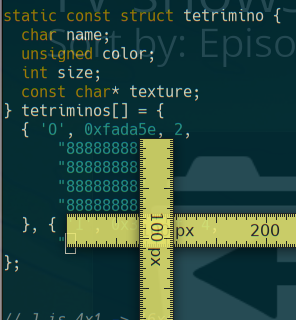
\includegraphics[width=.5\linewidth]{media/screenruler.png}
\caption{Font aspect ratios center around 0.5.}
\label{fig:aspectratio}
\end{figure}

We use two display rows per game row but four display columns per game column.
This reflects what is, at least on my display and font, pretty much a 0.5
aspect ratio (Figure~\ref{fig:aspectratio}).

\begin{listing}[!htbp]
\inputminted[]{C}{code/tetrimino-display.h}
\caption{Creating a single tetrimino (from~\texttt{tetrimino.c}).}
\label{list:tetrimino-display}
\end{listing}

There are a few essential things to
take away from Listing~\ref{list:tetrimino-display}:

\begin{denseitemize}
\item{Each time we call \texttt{ncplane\_putsimple()}, the cursor is advanced
      the expected amount. If we were calling \texttt{ncplane\_putegc()} with
      a multicolumn grapheme cluster, the cursor would be advanced multiple
      columns.}
\item{Between rows, we need move the cursor ourselves, since we're skipping over
      part of the plane (this isn't true for several of the pieces, but the
      cursor update is a trivial operation, not worth avoiding).}
\item{The cursor is always initialized to the origin of a new plane, and coordinates
      supplied to \texttt{ncplane\_} functions are relative to the plane,
      \textit{not} the terminal. Coordinates can be translated among planes
      using \texttt{ncplane\_translate()}.}
\item{We only have ASCII characters in the textures right now. Were we to
      introduce any multibyte UTF-8---and we may well do so, for e.\ g.\ the
      Box Drawing Characters---the \texttt{strlen()} we size our rows by here
      would no longer fly. We'd need use \texttt{mbstowcs()}, or redefine the
      textures as \texttt{wchar\_t} arrays and use \texttt{wcslen()},
      or change up our encoding\footnote{We go with the third option, as you'll see.}. \textfrench{\textit{Rien n'est simple, mais tout est facile\ldots}}}
\end{denseitemize}

\begin{listing}[!htbp]
\inputminted[]{C}{code/tetrimino-draw.h}
\caption{Distributing the tetriminos with ``flying-v'' technique (from~\texttt{tetrimino.c}).}
\label{list:tetrimino-draw}
\end{listing}

\begin{listing}[!htbp]
\inputminted[]{C}{code/tetrimino-main.h}
\caption{A one-shot, display-only \texttt{main()} (from~\texttt{tetrimino.c}).}
\label{list:tetrimino-main}
\end{listing}

Our \texttt{main()} sets the locale, initializes the terminal, and draws the
seven pieces (Listings~\ref{list:tetrimino-draw} and~\ref{list:tetrimino-main}).
Each piece has a one-letter name; for now, we draw with those glyphs. The
pieces are monochromatic. This renders familiar shapes in the correct colors
(Figure~\ref{fig:tetriminos-1}), but other than that, it's (like most classic
Curses programs) kinda fugly. I wouldn't want to play with these pieces.

\begin{figure}[!htbp]
  \centering
  \begin{minipage}{0.30\textwidth}
    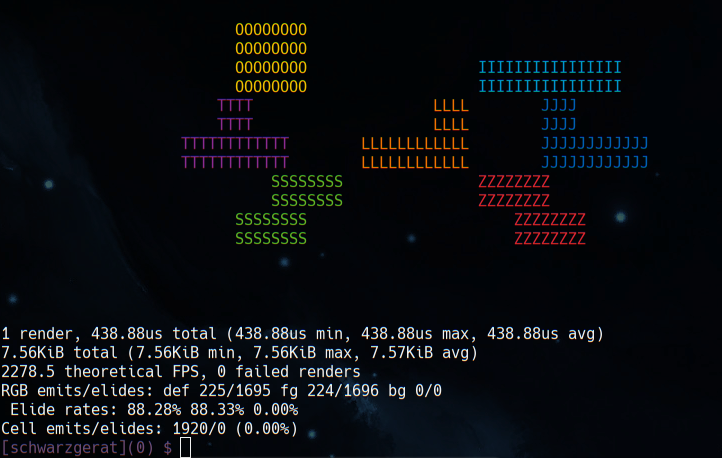
\includegraphics[width=1\linewidth]{media/tetriminos-1.png}
    \caption{Unspeakably foul.}
    \label{fig:tetriminos-1}
  \end{minipage}\hfill
  \begin{minipage}{0.30\textwidth}
    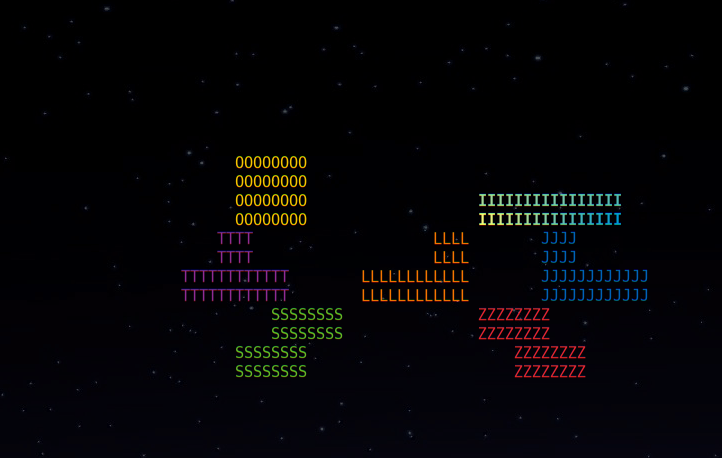
\includegraphics[width=1\linewidth]{media/tetrimino-gradient1.png}
    \caption{Adding a gradient.}
  \end{minipage}\hfill
  \begin{minipage}{0.30\textwidth}
    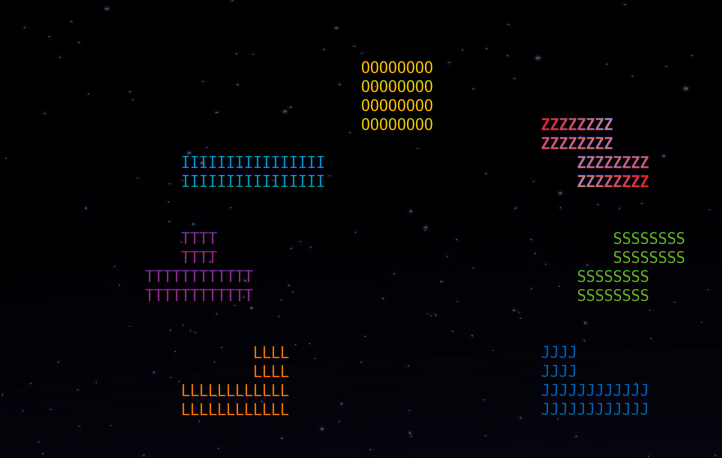
\includegraphics[width=1\linewidth]{media/tetrimino-gradient2.png}
    \caption{Linear expansion.}
  \end{minipage}\hfill
\end{figure}

This is hardly a render/event loop; in fact it's not a loop at all. If we were
using the alternate screen, we wouldn't see our output before flashing back to
the normal screen. Let's go ahead and hook up input. We'll be controlling one
of the tetriminos at a time---the selected piece will use boldface, and have its
color brightened\footnote{Note how we use two distinct indicators. On a monochromatic
display, we need the bold, and on a display which can't do bold, maybe we get a
color difference. Also, we want bold even if we have color, because until we
see the base color, there's no reason to think of the initial selection as
``bright''.}. We do so (Listing~\ref{list:tetrimino-switch}) with a pair of
helpers---\texttt{reduce()} and \texttt{highlight()}--- which drive the common
\texttt{blast()}. \texttt{blast()} makes use of two new functions,
\texttt{ncplane\_format()} and \texttt{ncplane\_stain()}. They allow the
attributes and channels, respectively, of a rectangular region to be changed
without altering other components. The corresponding glyph-only output routines
are likewise described in (Chapter~\ref{sec:staining}).

\begin{listing}[!htbp]
\inputminted[]{C}{code/tetrimino-switch.h}
\caption{Switching between pieces (from~\texttt{tetrimino-input.c}).}
\label{list:tetrimino-switch}
\end{listing}

While we're making things prettier, let's replace
those letters with some classy box-drawing characters, and improve on this
layout. We can do some simple algebraic extensions and get some linear spacing,
but it's just as easy to use trigonometric functions and get an approximation
to a circle. This is especially valuable as the terminal geometry changes; our
fixed linear scalings would break down as the display aspect changes, but a
good ol' circle will work on any sufficient radius
(Listing~\ref{list:tetrimino-drawcircle}).

\begin{listing}[!htbp]
\inputminted[]{C}{code/tetrimino-drawcircle.h}
\caption{Trigonometric layout: simpler, yet more accurate (from~\texttt{tetrimino-input.c}).}
\label{list:tetrimino-drawcircle}
\end{listing}

Since there's nothing else going on, it's trivial to process \texttt{stdin} in
a blocking fashion from our main thread. Let's add the code to track a selected
piece, visually highlight it, and process input (Listing~\ref{list:tetrimino-inputcore}).
The space bar will advance among the pieces in one direction,
and Tab in the other. The arrow keys and vi keys will translate the selected
piece in four directions. The parentheses will rotate the piece $\frac{\pi}{2}$ radians
clockwise and counterclockwise.

\begin{listing}[!htbp]
\inputminted[]{C}{code/tetrimino-inputcore.h}
\caption{Core input dispatch (from~\texttt{tetrimino-input.c}).}
\label{list:tetrimino-inputcore}
\end{listing}

Of course, when there's no other activity, things are easy. Quite often, we'll
have some periodic concurrent activity. Let's say we wanted to make the non-selected
tetriminos slowly rotate. The rotation isn't difficult; Notcurses provides
that functionality for you. But you don't want the rotation synced to input
activity, and you're hardly the kind of know-nothing what-not that would
busy loop on a nonblocking input interface, right? I hope you don't consider
yourself ``green'' if that's the case, because you're burning dinosaurs out
of sheer laziness. Let's do it right. There are of course four canonical
solutions to the problem of interleaving a set of asynchronous file descriptor-based
inputs against a set of periodic requirements; let's refresh ourselves:

\begin{denseitemize}
\item{No holds barred, take no prisoners state machine. No quarter asked.
    None given. Certainly the most \textit{enjoyable} choice of the four, the
    one closest to the nature of the machine, and the option with the most
    built-in job security. Casting off the crutch of the process scheduler, we
    execute in a single thread, carefully programming our
    \texttt{epoll()}\cite{epoll7} or \texttt{kqueue()}\cite{kqueue2} timeouts
    against a hierarchal, hashed timer wheel\cite{timerwheels}. As Alan Cox
    said, ``Computers are state machines. Threads are for people who don't
    understand state machines.''\footnote{Or did he? I can't find the original
    to cite. I wonder what the hell happened to Alan Cox.} Limited to a single
  CPU\ldots\ which probably isn't a problem here, but isn't exactly a great foundation
  on which to build our cathedral, \textfrench{\textit{n'est-ce pas?}}.}
\item{Two threads enter, one thread \texttt{exit()}s (hehehehe). We block on
    async I/O in our main thread. Another thread runs a timer wheel---for this,
    a loop around a \texttt{clock\_nanosleep()} will suffice. They
    lock against one another to avoid corrupting the screen or otherwise
    embarassing ourselves. The solution reeks of Java, but will work well
    enough, and any programmer---maybe even a Java programmer---ought be able
    to walk in and pick it up.}
\item{POSIX signaled timers. Noooooooooooooooooooooooooooooooooooooo.}
\item{Timer I/O multiplexing. Probably the best solution for a program of true
    scope, and in no way unfit for the task at hand. On Linux, you'll want
    \texttt{timerfd\_create()} and friends. On FreeBSD, look for \texttt{EVFILT\_TIMER}.
    Throw that into the appopriate I/O multiplexor call, spin it out among a
    few threads if you feel so inclined\cite{libtorque}, and call it a day.
  The only real disadvantage here is a lack of portability.}
\end{denseitemize}

Some will ask, ``Sounds dank, but what about on this shiny operating system I
purchased from Applooglesoft? Look, I can speak to it! Sirana, diminish my
freedoms and spy on me!'' I could give two shits about your closed-source
operating system. I presume you can purchase cloud-based Timers as a Service
(TaaS) or something.

We can now cycle through the pieces, and move the piece we've selected around
on the screen. Grab one and move it towards another piece. Experimentation will
reveal that each piece has a~\gls{boundingbox}, that there is a total ordering
among the seven pieces, and that a piece below another piece's bounding box is
robbed of its color (Figure~\ref{fig:tetrimino-badplane}). Recall from
Chapter~\ref{sec:rendering} how we solve for each coordinate of the display
grid: the EGC is a dimension distinct from the coloring channels. Each of the
planes we create is rectilinear, with the piece drawn using Unicode
\texttt{U+2588 FULL BLOCK}, and the other cells left unwritten. The foreground
for our pieces is an RGB color, and for the other cells is the default terminal
color. Upon intersecting with a lower plane, the lower plane's EGC is chosen for
rendering, but the foreground color is default terminal color (white in my
example). So the piece underneath flipping to white while another piece is
nearby makes perfect sense. The solution is simple: we set the foreground
transparent for the base character of each plane. Foreground calculation will
now bypass the plane where we haven't drawn, and the distorted plane regains
its expected colors (Figure~\ref{fig:tetrimino-trans}). Takeaway: by default, planes
obstruct only color, not glyphs.

\begin{figure}[!htbp]
  \centering
  \begin{minipage}{0.30\textwidth}
    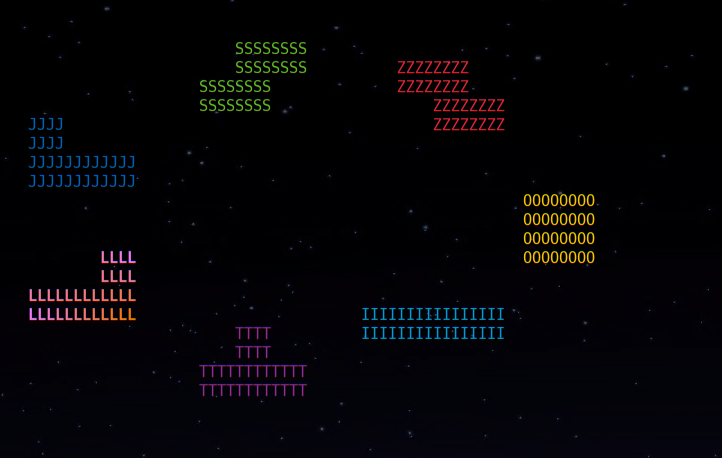
\includegraphics[width=1\linewidth]{media/tetrimino-gradient3.png}
    \caption{Trigonometry!}
  \end{minipage}\hfill
  \begin{minipage}{0.30\textwidth}
    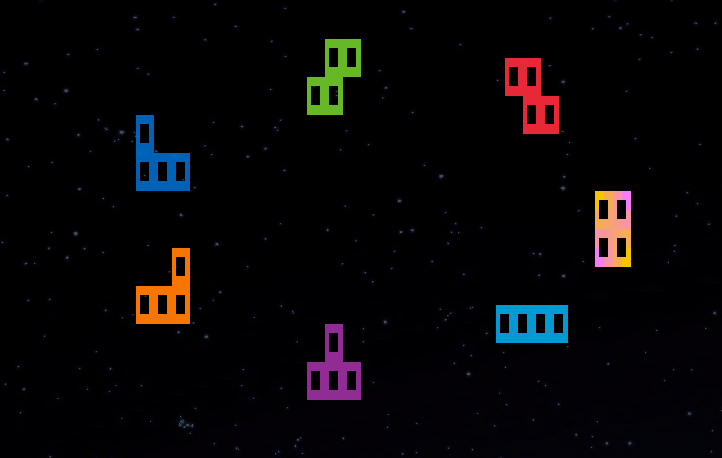
\includegraphics[width=1\linewidth]{media/tetrimino-gradient4.png}
    \caption{Unicode Blocks.}
  \end{minipage}\hfill
  \begin{minipage}{0.30\textwidth}
    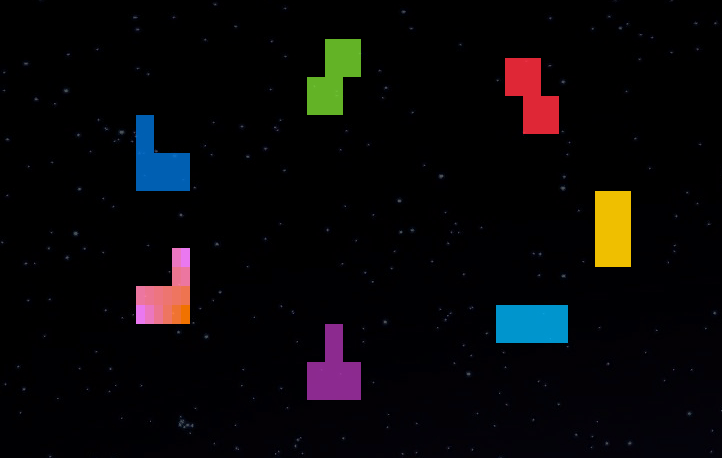
\includegraphics[width=1\linewidth]{media/tetrimino-gradient5.png}
    \caption{Better blocks.}
  \end{minipage}\hfill
\end{figure}

\begin{figure}[!htbp]
  \begin{minipage}{0.30\textwidth}
    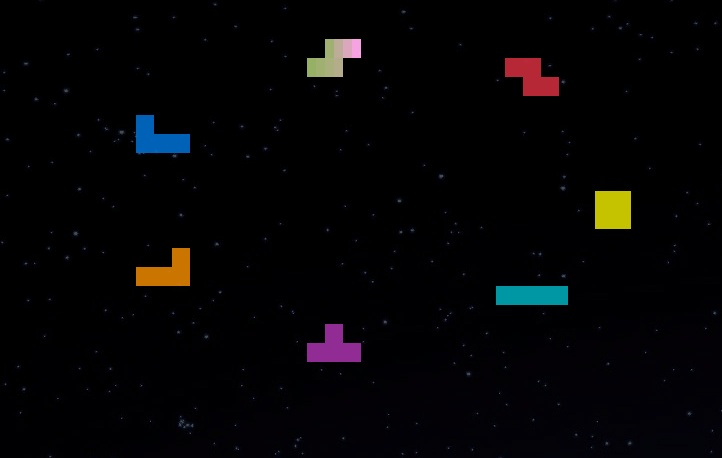
\includegraphics[width=1\linewidth]{media/tetrimino-gradient6.png}
    \caption{Adjusting for cell aspect ratio.}
  \end{minipage}\hfill
  \begin{minipage}{0.30\textwidth}
    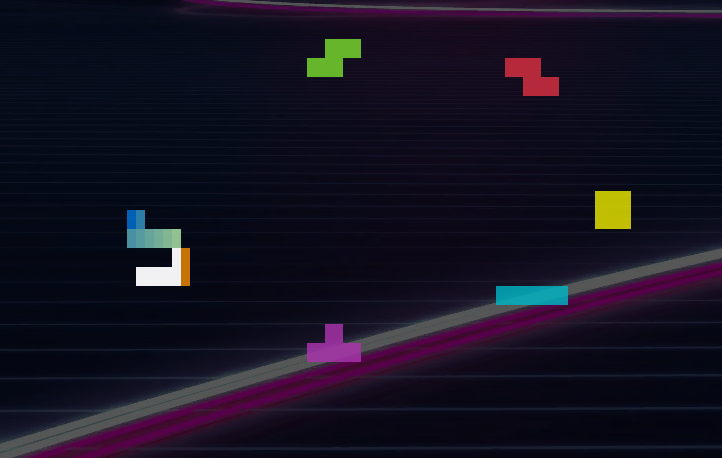
\includegraphics[width=1\linewidth]{media/tetrimino-gradient7.png}
    \caption{Undesirable plane interaction.}
    \label{fig:tetrimino-badplane}
  \end{minipage}\hfill
  \begin{minipage}{0.30\textwidth}
    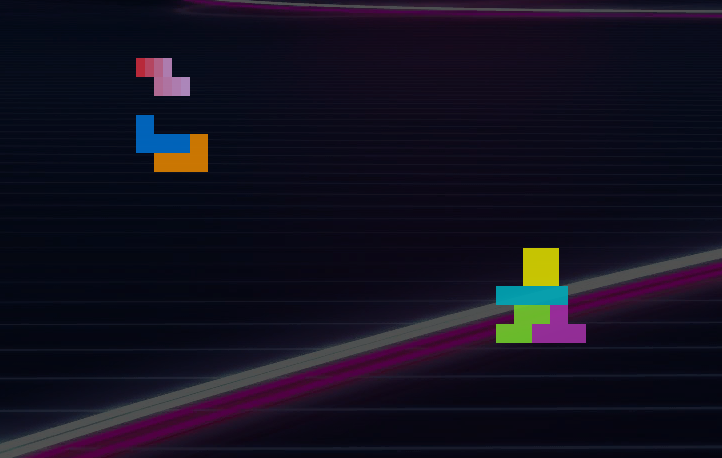
\includegraphics[width=1\linewidth]{media/tetrimino-gradient8.png}
    \caption{Resolve it with transparent planes.}
    \label{fig:tetrimino-trans}
  \end{minipage}\hfill
\end{figure}

\begin{listing}[!htbp]
\inputminted[]{C}{code/tetrimino-databox.h}
\begin{minted}{C}

\end{minted}
\inputminted[]{C}{code/tetrimino-displayutf8.h}
\caption{Improving appearance with Unicode Block Elements (from~\texttt{tetrimino-input.c}).}
\label{list:tetrimino-displayutf8}
\end{listing}

Adding a background image is simple. We'll render it to the standard plane, our
``background'' for now (remember, newly created planes are placed at the top of
the z axis). Despite decoding the image \textit{after} creation of the pieces,
the pieces are thus not hidden. There is no need to inform Notcurses of the
image's format, nor parameters thereof. Simply provide the file name and target
rendering plane, and we're off. See Chapter~\ref{sec:libav} for a full treatment
of multimedia in Notcurses.

\begin{listing}[!htbp]
\inputminted[]{C}{code/tetrimino-background.h}
\caption{Throwing in a background (from~\texttt{tetrimino-input.c}).}
\label{list:tetrimino-background}
\end{listing}

To rotate the unselected pieces, we'll go ahead and spawn a POSIX thread. We'll
thus need lock against piece selection. We've been leaving all the end-of-process
cleanup in the capable hands of~\texttt{notcurses\_stop()}, but it can't go
terminating threads for us, and it in any case wouldn't be safe to do so while
said thread was calling into Notcurses! First, add a marshaling struct to share
some state (Listing~\ref{list:tetrimino-tetmarsh}). We'll use POSIX
cancellation\footnote{Which isn't anywhere near as bad as it's sometimes made out to be.
Find the places where you don't want to be cancelled. Each such place needs a
cleanup handler pushed/popped around it, or cancellation disabled for its
breadth. Things get a little counterintuitive with
cancellable-but-uninterruptible system calls, but that's nothing if you came up
on BSD signals. It's hardly the most offensive wart on the great hairy ass
that is ANSI/ISO C, and---heresy, I know---I honestly prefer (most of) the
POSIX model to (most of)
the threading introduced in \CC11.} to blast the rotator thread, and~\texttt{pthread\_join()}
it to ensure safe passage through shutdown.

\begin{listing}[!htbp]
\inputminted[]{C}{code/tetrimino-tetmarsh.h}
\caption{Marshaling structure for shared state (from~\texttt{tetrimino-input.c}).}
\label{list:tetrimino-tetmarsh}
\end{listing}

\begin{listing}[!htbp]
\inputminted[]{C}{code/tetrimino-thread.h}
\caption{Spin them doggies (from~\texttt{tetrimino-input.c}).}
\label{list:tetrimino-thread}
\end{listing}

As a final touch, let's slide a dark, translucent plane underneath the
selected piece, making it more visible. We create this plane prior to the
pieces, ensuring it's below all of them (but above the background). We set it
black, and its alpha to \texttt{CELL\_ALPHA\_BLEND}. This way it won't entirely
block out the background underneath the selected piece, but it will dim it,
its black blending into the grey tones underneath. The piece is unaffected.

\begin{listing}[!htbp]
\inputminted[]{C}{code/tetrimino-box.h}
\caption{Set the selection off with a coaster (from~\texttt{tetrimino-input.c}).}
\label{list:tetrimino-box}
\end{listing}

\begin{figure}[!htbp]
  \centering
  \begin{minipage}{0.30\textwidth}
    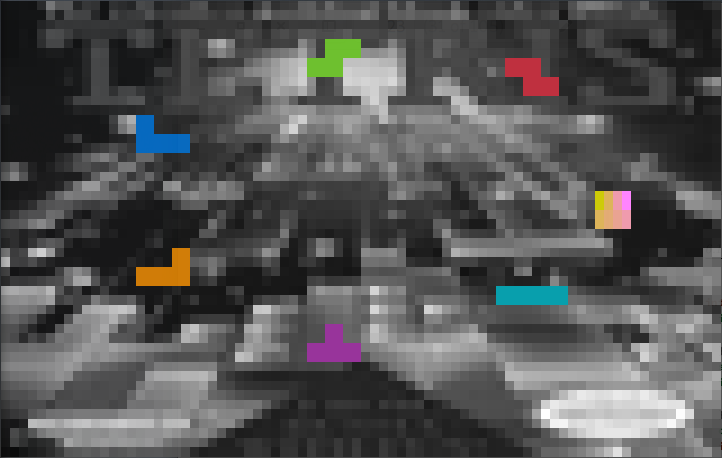
\includegraphics[width=1\linewidth]{media/tetrimino-bg.png}
    \caption{Background image, greyscaled.}
    \label{fig:tetrimino-bg}
  \end{minipage}\hfill
  \begin{minipage}{0.30\textwidth}
    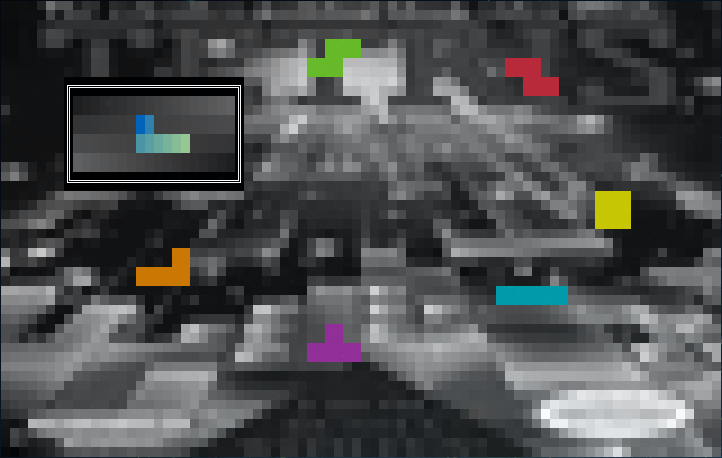
\includegraphics[width=1\linewidth]{media/tetrimino-bgbox.png}
    \caption{Opaque highlight box.}
  \end{minipage}\hfill
  \begin{minipage}{0.30\textwidth}
    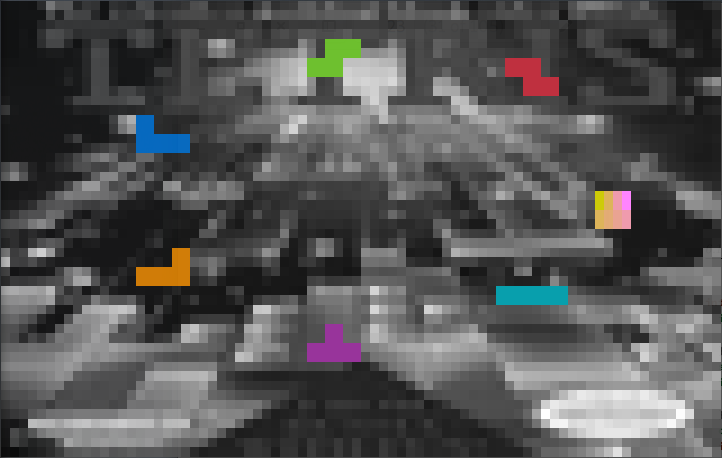
\includegraphics[width=1\linewidth]{media/tetrimino-bg.png}
    \caption{Rotation thread enabled\textbf{FIXME}.}
  \end{minipage}\hfill
\end{figure}

\begin{listing}[!htbp]
\inputminted[]{C}{code/tetrimino-inputmain.h}
\caption{Putting it all together (from~\texttt{tetrimino-input.c}).}
\label{list:tetrimino-inputmain}
\end{listing}

\pagebreak
\newpage
%%%%%%%%%%%%%%%%%%%%%%%%%%%%%%%%%%%%%%%%%%%%%%%%%%%%%%%%%%%%%%%%%%%%%%%%
\section{Terminal mechanics}
\label{section:tty}
\epigraph{The tty layer is one of the very few pieces of kernel code that scares the hell out of me.}{Ingo Molnar\cite{molnarhell}}
You won't often need to deal with the gritty details of terminal access and
manipulation. It's still important to understand what's going on behind the
abstraction, especially for when things go wrong. As was made clear in
Chapters~\ref{sec:direct} and~\ref{sec:fullscreen}, Notcurses requires a
proper terminal definition and a handle to a terminal device, or initialization
will fail (NCURSES requires the same). With that said, the UNIX terminal layers
have never been, and are not now for the faint of heart\footnote{When Ingo
Molnar is scared, we all ought be scared.}. Extending back to the AT\&T dark
ages (and with at least three major distinct interfaces over the years, only unified
in 1997's SUS2), they are configured primarily through messy \texttt{ioctl}s and the
slightly-less-messy \texttt{termios} API.

More details than you probably want are available from Chapters 18 and 19 of \cite{apiue}
(general UNIX), Chapters 62 and 64 of~\cite{linuxprogramming} and Chapter 18
of~\cite{linuxdevicedrivers} (Linux), and Chapter 10 of~\cite{freebsddesign} (FreeBSD).

Modern workstations support a variety of physical and virtual terminal devices:
\begin{denseitemize}
\item{Honest-to-Bog serial terminals, probably using the RS-232\cite{rs232}
      protocol over a D-subminiature 25-pin (DB-25M) or 9-pin (DE-9M)
      connector (see Table~\ref{table:serial}).}
\item{Virtual consoles on text-based video, plus a keyboard.}
\item{Virtual framebuffer consoles on graphics-based video, plus a keyboard.} 
\item{Terminal emulators in a graphical environment, plus brokered input devices.}
\item{Pseudoterminals hooked up to network connections.}
\end{denseitemize}

\begin{table}[!htb]
  \centering
  \begin{tabular}{ |c|c|c|c|c| }
    \hline
    Signal & DB-25M & TIA-574 DE-9M & Yost 8P8C\cite{yost} & Originator \\
    \hline
    \hline
    Protective ground & 1 & x & x & x \\
    \hline
    Transmitted data & 2 & 3 & 3 & DTE \\
    \hline
    Received data & 3 & 2 & 6 & DCE \\
    \hline
    Request to send & 4 & 7 & 1 & DTE \\
    \hline
    Clear to send & 5 & 8 & 8 & DCE \\
    \hline
    Data set ready & 6 & 6 & 2 & DCE \\
    \hline
    Signal ground & 7 & 5 & 4, 5 & x \\
    \hline
    Carrier detect & 8 & 1 & 2 & DCE \\
    \hline
    Data terminal ready & 20 & 4 & 7 & DTE \\
    \hline
    Ring indicator & 22 & 9 & x & DCE \\
    \hline
  \end{tabular}
  \caption[RS-232/EIA-232 pin mappings]{RS-232/EIA-232 pins (DCE=Data circuit equipment, DTE=Data terminal equipment)}
  \label{table:serial}
\end{table}

On Linux, three kernel definitions form the core of the terminal abstraction
(the ``tty layer''). A \texttt{tty\_driver} function interface exists for each
tty implementation, and each has a different corresponding
major+minor device number pair. These implementations are enumerated in
\texttt{/proc/tty/drivers} (sample contents are listed in Table~\ref{table:procttydrivers}).
Line disciplines can be found in \texttt{/proc/tty/ldiscs}. The only line discipline
you're likely to encounter in a terminal context is \texttt{n\_tty}, the ``new tty''
discipline responsible for implementing ``cooked mode''\cite{essentialdrivers}.

POSIX.1-2017\cite{posix2017} §10.1 ``Directory Structure and Devices''
specifies three special files in the \texttt{/dev} directory, of which two are
related to the terminal/console system: \texttt{/dev/tty} is, within a process
context, a synonym for the controlling terminal associated with that process's
group (this can also be acquired with \texttt{tty(1)} or the POSIX C function
\texttt{ctermid(3)}\footnote{\texttt{/dev/tty} also uniquely supports the
\texttt{TIOCNOTTY} \texttt{ioctl(2)} for detaching a process from its
controlling terminal.}. The tty associated with an arbitrary file descriptor can
be retrieved with \texttt{ttyname\_r(3)}). \texttt{/dev/console} is a generic name for the current system console\footnote{Defined in \textit{ibid.} §3.392
``System Console'' as the device receiving messages sent by the \texttt{syslog()}
function. On Linux, it will also reproduce messages written to \texttt{/dev/kmsg}\cite{dmesg}.};
POSIX requires that the system console implement its ``General Terminal Interface'' (see
\textit{ibid.} §11). The standard console will by default be \path{/dev/tty0}, but this
can be changed with the \texttt{console=} kernel command line parameter, or with
an explicit \texttt{ConOut} UEFI variable (see §11.4 of \cite{uefi}). \texttt{/dev/tty0} is a special device on Linux linked to
the current virtual console (which might not be the system console). The
available system consoles can be found in \texttt{/proc/consoles}.

Initial \texttt{/dev/ttyN} devices are created internally by the kernel
(according to the value of \texttt{MAX\_NR\_CONSOLES}, by default 64) and set
up by \texttt{udev}. These are distinct devices, each usable by one virtual
console. Serial consoles show up as \texttt{/dev/ttySN}\cite{ttys4}. Each
virtual console gets a device at \texttt{/dev/vcsN} allowing access to the
glyph values of the console, a device at \texttt{/dev/vcsaN} allowing access to
the attributes at each cell, plus screen geometry, and a device at \texttt{/dev/vcsuN}
providing access to the Unicode values of each cell\cite{vcs4}. If a framebuffer console
is being used, these devices are prepared atop some framebuffer device \texttt{/dev/fbN} (see
Figure~\ref{fig:framebuffers}); these mappings can be managed with \texttt{con2fbmap(1)}.

\begin{figure}[!htb]
  \centering
  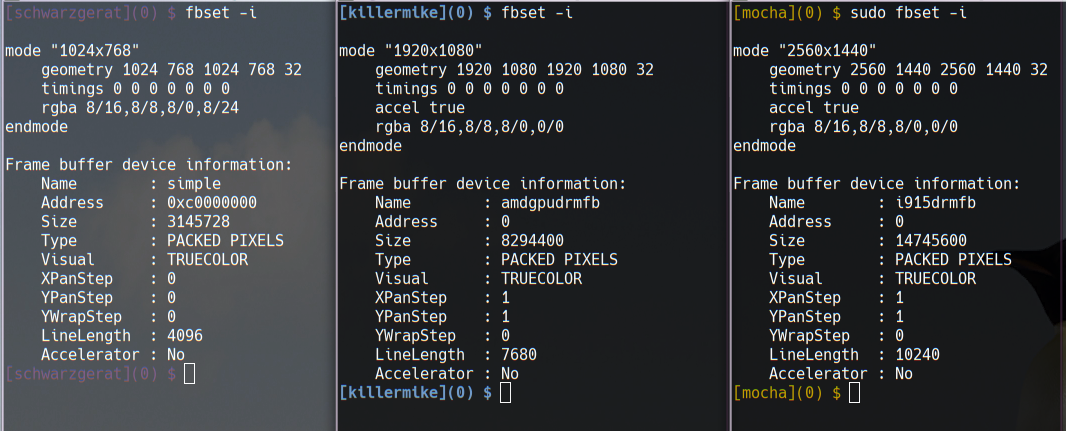
\includegraphics[width=.75\linewidth]{media/framebuffers.png}
  \caption{Three different Linux framebuffer implementations.}
  \label{fig:framebuffers}
\end{figure}

\begin{table}[!htb]
  \centering
  \begin{tabular}{ |c|c|c|c|c|c| }
    \hline
    Name & Default node & Major & Minor & Type & sysfs \\
    \hline
    \hline
    /dev/tty & /dev/tty & 5 & 0 & system:/dev/tty & devices/virtual/tty/tty* \\
    \hline
    /dev/console & /dev/console & 5 & 1 & system:console & devices/virtual/tty/console \\
    \hline
    /dev/ptmx & /dev/ptmx & 5 & 2 & system & devices/virtual/tty/ptmx \\
    \hline
    /dev/vc/0 & /dev/vc/0 & 4 & 0 & system:vtmaster & x \\
    \hline
    usbserial & /dev/ttyUSB & 188 & 0--511 & serial & x \\
    \hline
    serial & /dev/ttyS & 4 & 64--95 & serial & x \\
    \hline
    rfcomm & /dev/rfcomm & 216 & 0--255 & serial & x \\
    \hline
    pty\_slave & /dev/pts & 136 & 0--1048575 & pty:slave & x \\
    \hline
    pty\_master & /dev/ptm & 128 & 0--1048575 & pty:master & x \\
    \hline
    unknown & /dev/tty & 4 & 1--63 & console & devices/virtual/tty/console \\
    \hline
  \end{tabular}
  \caption[Expanded contents of \texttt{/proc/tty/drivers}]{Extended content of a sample \texttt{/proc/tty/drivers}\\
    (5.5.6 kernel. \texttt{sysfs} information has been added)}
  \label{table:procttydrivers}
\end{table}

The various termios flags allow very fine control of the kernel state associated
with a given terminal. It is possible to mix flag settings arbitrarily, but three
modes are common, and have their own nomenclature:
\begin{denseitemize}
\item{\textbf{Canonical mode, aka cooked mode:}   The terminal driver buffers input until a newline is entered, while echoing
    it to the screen. Ctrl+C is mapped to \texttt{SIGINT}, Ctrl+\textbackslash\ is
    mapped to \texttt{SIGQUIT}, and Ctrl+Z is mapped to \texttt{SIGTSTP}.
    Buffered input is flushed when these signals are sent. The default mode.}
\item{\textbf{Cbreak mode:} Line buffering is disabled, as is the processing
  of erase/kill characters. Interrupt and flow control translation is unaffected.
Sometimes referred to as \textit{rare mode}. This mode allows processing of input
without waiting for a newline character, while retaining e.g. Ctrl+C.}
\item{\textbf{Raw mode:} Interrupt and flow control translation is also disabled.
  This allows all keyboard input to be processed without preprocessing by the
  line discipline, but e.g. Ctrl+C behavior is lost, and (if desired) must be
  emulated in user space.}
\end{denseitemize}

In addition to these physically-backed devices, ptys---pseudoterminal devices\cite{pty7}---exist
to support virtual teletype functionality, wherein a process plays the role
of hardware. Pseudoterminals\footnote{You might
 hear about both System V and BSD pseudoterminals. SUS standardized around
the System V form, known on Linux as ``UNIX 98''. This term refers to 1997's
SUSv2 ¯\textbackslash\_(ツ)\_/¯. Trash BSD ptys look like \texttt{/dev/ttyLN} and \texttt{/dev/ptyLN}.}
back most terminal instances, including GUI terminal emulators, network
services such as SSH, and multiplexers such as \texttt{screen}. A pty provides a
bidirectional channel between a \textit{master} and \textit{slave}, with the
slave presenting a classic terminal interface (i.e. writing a Ctrl+C to the
master side will (under the cooked or cbreak disciplines) result in
\texttt{SIGINT} being delivered to the foreground process group.

The details of Linux pseudoterminal pair creation can be found on the \texttt{pts(4)}\cite{pts4} man page.
\texttt{posix\_openpt(3)}\cite{posixopenpt3} opens the ``master clone device''
\path{/dev/ptmx}, receiving a file descriptor corresponding to the new PTM (pseudoterminal master).
A new PTS (pseudoterminal slave) is created in \path{/dev/pts/}
\footnote{\path{/dev/pts} is typically its own \texttt{devpts} filesystem on Linux.}, whose name can be discovered by
providing the PTM file descriptor to \texttt{ptsname\_r(3)}\cite{ptsname3}.
Opening this PTS requires use of the \texttt{grantpt(3)} and \texttt{unlockpt(3)} calls.
Once both sides have been opened, data freely flows between the PTM and PTS.

You generally shouldn't need to be mess with TTYs or PTYs yourself as an
application developer, but now you know what all that junk clogging up
your \path{/dev} is. Some day when you mess up your initramfs, and
you're getting an error message like ``\path{/dev/ptmx} does not exist you have
no chance to survive make your time'' you'll know you're missing the
master clone device, some small consolation as you hopelessly reboot\footnote{Pro tip:
should you ever need supply input to programs which refuse to read from pipes
(e.g. \texttt{passwd}), you can pump the input through a named pty.}.

\subsection{Terminals and the UNIX process model}
\label{sec:unixprocs}

Understanding how these devices---physical or virtual---end up connected to
actual processes requires understanding some basic details of the UNIX
process model\footnote{For a more complete description, consult Chapter 9
of \cite{apiue}.}. Recall the UNIX principle that ``everything is a file''. Generally---and
this is true for all terminal devices---devices will be \texttt{open(2)}ed
using their \path{/dev} nodes, and then operated upon as a typical file
descriptor. You're no doubt aware that UNIX programs traditionally start with
at least three file descriptors open: 0 for \texttt{stdin}, 1 for
\texttt{stdout}, and 2 for \texttt{stderr}. Recall further that file descriptors
are by default not closed across an \text{exec(2)} call that replaces one
process's code with another object.

Each process has a process ID (PID) unique to its PID namespace (see
\texttt{clone(2)}\cite{clone2}, particularly the \texttt{CLONE\_NEWPID} flag).
Each process is a member of a \textit{process group}, and each process group
has its own process group ID (PGID)\footnote{Both PIDs and PGIDs are represented using \texttt{pid\_t}.}.
This PGID is equal to the \textit{group leader}'s PID, and each process group
has one and only one leader. Signals can be addressed to a process group by
supplying the negative PGID to e.g. \texttt{kill(2)}; a signal sent to a group
will be delivered to all processes of that group. One of the most common
scenarios in which multiple processes are kept in a single group is a shell
pipeline (a \texttt{fork(2)}ing process will usually place independent children
into a new process group). This is the essential facility underlying job control
(placing a job into the background, etc.), explaining why backgrounding
applies to an entire pipeline. Processes may be moved between process groups,
but only within a \textit{session}.

All process groups (and thus all processes) are members of some session. Each
session has a session ID (SID)\footnote{This session ID isn't really its own
unique value---it's implied by the session leader process.}. This SID
is the same as the PID of its \textit{session leader}. A session might or might
not have a controlling terminal (daemons disconnect themselves from their
controlling terminal). Login sessions almost always do have a controlling
terminal: the tty on which \texttt{login} was running (for a cosole session),
or the pty opened at process creation (for e.g. SSH or \texttt{xterm}). The
process groups of a session are divided into a single \textit{foreground group}
and zero or more \textit{background groups}.

Figure~\ref{fig:termprocs} shows the terminal-connected processes on one of
my Linux workstations, with their PIDs, PPIDs (parent process IDs), PGIDs
and SIDs. \texttt{agetty} is listening on tty1, spawned by
\texttt{init} (process 1). Xorg is sitting on tty7, having been spawned by a
display manager (which is \textbf{not} itself connected to a terminal). The
\texttt{bash} at PID 41599 is the child of a \texttt{screen} process.
\texttt{bash} at PID 846497 is a child of \texttt{sshd}.

\begin{figure}[!htb]
  \centering
\begin{verbatim}
[killermike](0) $ ps  --ppid 2 --deselect o pid,ppid,pgid,sid,tty,comm  | grep -v ?
    PID    PPID    PGID     SID TT       COMMAND
  41599   41598   41599   41599 pts/1    bash
  41654   41599   41654   41599 pts/1    rtorrent main
 510181       1  510181  510181 tty1     agetty
 510609  510187  510609  510609 tty7     Xorg
 846497  846495  846497  846497 pts/0    bash
 851850  846497  851850  846497 pts/0    ps
 851851  846497  851850  846497 pts/0    grep
[killermike](0) $
\end{verbatim}
\caption{Terminal-connected processes on a Linux machine.}
\label{fig:termprocs}
\end{figure}

Sessions affect how signals from the terminal are distributed. \texttt{SIGINT}
and friends (signals generated due to the line discipline) are sent to the
foreground process group. Only the foreground process can read from the
terminal; if a background process attempts to do so, it is sent \texttt{SIGTTIN}, the default
handler of which is to stop. A stopped background process will receive
\texttt{SIGCONT} when brought into the foreground. Likewise, a background
process will be sent \texttt{SIGTTOU} if it attempts to write to the terminal
when the TOSTOP tty flag is valid, or attempts to reconfigure the terminal in
any way\cite{sigterminals}.

Finally, it's worth knowing how terminals get turned into login sessions. Under
\texttt{systemd-logind}\cite{logind}, \texttt{agetty} processes are launched
on demand (i.e.\ on first transition to the virtual console), on \texttt{ttyN}
through the value of \texttt{NAutoVTs}. Should you be so unfortunate as to
still be running SysVinit in 2020, ttys are configured in \path{/etc/inittab}\footnote{If you're one of those people who pine for SysVinit, your opinions are bad, and you should feel bad.}.
On FreeBSD, \path{/etc/ttys} plays a similar role\cite{fbsdttys5}. \texttt{getty},
\texttt{agetty} et al condition the line (if necessary), prompt for a login
name, and then invoke \texttt{login} or a similar program. \texttt{login} prompts
for a password (or \texttt{sshd} performs authentication by myriad means), and
if the user is authenticated, \texttt{exec(2)s} a login shell as a new session.
This login shell inherits the terminal file descriptors from parent processes,
and passes them (by default) to its children.

Environment variables are also inherited across process boundaries, and by the
time the login shell is run, the all-important \texttt{LANG} and \texttt{TERM}
variables ought have been set. \texttt{LANG} defaults are based off the contents
of \path{/etc/locale.conf}. \texttt{TERM} is generally set by the terminal emulator itself,
or by \texttt{getty} on the console, and it is always forwarded by ssh\footnote{There is an exception; ssh does not forward \texttt{TERM} when the \texttt{-T}
parameter explicitly inhibits pty allocation.}. It's critical to have a correct \texttt{TERM}
value, and misinformation on configuring it runs rampant. Besides the NCURSES FAQ\cite{ncursesfaq},
I find the nosh project's \texttt{TERM} page\cite{noshterm} to be an excellent
resource, along of course with the \texttt{term(7)} man page\cite{term7}. You
will likely want to manually ensure that \texttt{COLORTERM} is properly defined
for 24-bit TrueColor, assuming your terminal supports it.

\begin{figure}[!htb]
  \centering
  \includegraphics[width=.75\linewidth]{dot/tty-serial.png}
  \caption{A serial console, from hardware to userspace.}
  \label{fig:ttysetups}
\end{figure}

Figure~\ref{fig:ttysetups} is adapted from those of \cite{ttydemystified}.

\subsection{Escape codes ANSI and otherwise}
\label{sec:escapes}

In a relic from teletypes, ISO 646, ISO 2022, and ECMA-35 described use of
non-destructive backspace to produce composed characters from spacing ones.
This had been eliminated by ISO 4873, ECMA-43, and ISO 8859.

\textbf{FIXME FIXME other stuff}

\pagebreak
\newpage
%%%%%%%%%%%%%%%%%%%%%%%%%%%%%%%%%%%%%%%%%%%%%%%%%%%%%%%%%%%%%%%%%%%%%%%%

\section{Character encodings and glyphs}\label{section:unicode}
\label{sec:charsets}
\epigraph{Thou whorseon zed, thou unnecessary letter!}{Wiliam Shakespeare, \textit{King Lear}}
We'll be well-served by becoming familiar with our core building
blocks---character sets and their rasterized forms. Even if we were to shrink
the character cell to a single pixel, we'd still need write one or another
character into it, and emit a control code to stylize it\footnote{I've seen
this idea bandied about as if it's a serious suggestion. Besides the fact
that it won't work in a console, escapes are \textit{far} less efficient than
canvases or OpenGL display lists; if your plan involves using ANSI escape
sequences to drive a 1920x1080 display via roughly two million 1x1 character
cells, you're not going to space today, or maybe ever\cite{upgoerfive}.}.

In the beginning, there are somewhat Platonic \textit{characters}, one of the
most imprecise terms in all of computer science (even when we leave aside the
data type \texttt{char}). In and of itself, a character is nothing more than an
identifier: \texttt{LATIN CAPITAL LETTER I}\footnote{Isn't that a recursive
definition? You betcha.}. There are many things a character is not:

\begin{denseitemize}
\item{A character is not necessarily unique within a character set (see diacritic vs.\ precomposed forms).}
\item{Different characters needn't be distinct glyphs\cite{nothinggoesaway}.}
\item{A character needn't limit itself to a single column, even when using a fixed-width font.}
\item{A character does not necessarily have a visual representation.}
\item{A character does not necessarily have a single meaning among different languages.}
\item{In a given encoding, all characters are not necessarily the same size.}
\item{A character cannot necessarily capture the state of the keyboard at some time.}
\item{A character cannot necessarily describe a cell of a display at some time.}
\end{denseitemize}

Collecting characters and assigning them distinct (not necessarily contiguous or
even ordered) numbers creates a \textit{code set}, and the smallest contiguous
range of numbers covering this code set is a \textit{code space}. The Unicode 13
code space is comprised of 17 contiguous planes of 65,536 code points each, for
a size of $17*2^{16}$. It defines 143,859 characters, smaller than its
code space by an order of magnitude. A map from a code set to a set of bit
sequences is a \textit{character encoding}. There are numerous standard
encodings of the Universal Character Set, each of which represents the entire
set in different ways (the best one is UTF-8, as we will see). Character sets
are registered with IANA per RFC 2978\cite{rfc2978}, and character encodings
are registered with ISO Register of Coded Characters per ISO/IEC
2375\cite{iso2375}.

Character graphics are formed from \textit{glyphs}, the visual renderings of a
character encoding, supplied by a font. These glyphs might fuse into what
Unicode Standard Annex \#29\cite{annex29} refers to as a \textit{user-perceived
character} or \textit{grapheme cluster}. A formal algorithm for dividing a
stream of glyphs into grapheme clusters (``horizontally segmentable units of
text\cite{meaningcodepoints}'') achieves \textit{segmentation}. The current
Unicode segmentation algorithm yields \textit{extended grapheme clusters}.

These extended grapheme clusters (EGCs) can be thought of as the atoms of
character graphics. It is not generally possible to write them partially, nor
to partially overlay one atop another. Backspacing ought usually remove entire EGCs
at a time. The cursor ought cross an EGC in a single movement. In Notcurses,
each cell of a plane can hold a single EGC, which must be written as a single
unit. The actual number of columns occupied by an EGC is a property of the font
and layout engine being used.

In the modern era, Unicode is used just about everywhere, and programs must be
prepared to handle it. On the plus side, Unicode presents a single, coherent
means of representing all the world's languages, eliminating the old necessity
of switching among encodings at runtime. UNIX has its origins---and most of its
modern UI---in a much smaller character set: ASCII.

\subsection{Everyone loves ASCII}
\begin{wrapfigure}{O}{.5\textwidth}
  \fbox{%
    \parbox{0.5\textwidth}{
In the early 1960s, an IBM employee on a dare ate a hallucinogenic tapeworm
that pissed nitric acid. Stuffing his steaming, rapidly decoiling bowels
up into a brown paper bag, he was off to the hospital. Alas! On those very
hospital steps he was struck by lightning, and filled with spears, and
set upon by savage hogs, and finally exploded. The tapeworm emerged, clad
in shimmering mandorla, with a name pronounceable by no human tongue. ``Adding
hallucinogenic tapeworms to a late project only makes it later,'' cautioned Fred
Brooks\cite{mythicalman}, but Gene Amdahl knew no peace. ``This
Tapeworm Queen reminds me of halcyon Wisconsin days!'' he cried, and on a prototype
Model 30 appeared her Name. Struck by the power of that Name, all began to bow,
and to weep. She vomited forth the Tapeworm Gospel. Looking upon this filth, they
thought it Good.\\
So now you know what EBCDIC is. There ended up being no fewer than 57
variants\cite{searle} of EBCDIC, worthy of Heinz. We will speak of it no
further. If you find yourself needing more information about EBCDIC, think long
and hard about your life decisions.}%
  }
\end{wrapfigure}
The first digital codes were the English telegraph system of Charles Wheatstone
and William Cooke, and American Samuel Morse's code, with which he famously
signaled ``What hath God wrought!'' in 1837. The Morse system was simpler, running
over a signle line, and quickly won out. The teleprinter of Jean-Maurice-Émile Baudot
(from whom we derive the modern unit \textit{baud}) followed in 1874, with its pentabit,
fixed-length Baudot code. Baudot code required 7.42 bittimes per character; at
a typical 0.022s bittime, it could transmit just over 6 characters per second\cite{martin}.

For our purposes, the story can reasonably start with a 7-bit encoding of
128 characters: ANSI X3.4-1986, perhaps better known as ASCII (Table~\ref{table:ascii}).
The first ASCII we would recognize as such\footnote{To paraphrase G.\ H.\
Hardy, ``ASCII-1963 was clever schoolboys; '68 a Fellow from another
College\cite{ghhardy}.''} was the unpublished ASCII-1965. The ASA (ANSI
before it was ANSI) ASCII 1963 didn't even have miniscules\footnote{Uppercase
and lowercase are loanwords from printing, where the two sets were
stored in different cases of the typesetting table. ``Majuscules'' and
``miniscules'' will mark your good breeding.}. ASCII-1968 was
released as USAS X3.4-1968 to wild acclaim. The ISO/IEC 646 standard\cite{iso646}
``internationalized'' ASCII-1968 by opening up 12 graphic characters to
regional specifications (the US ASCII defined the ``International Reference
Variant'')\cite{aivosto}.

The first 32 values are non-printable control codes, first given their current
definitions in ASCII 1968. These 32 codes (known as the ``C0'' coded control
set since ISO/IEC 646) lived on through ISO/IEC 2022 (ECMA-35), ISO/IEC 6429
(ECMA-48), ISO/IEC 8859 (ECMA-94), and are reproduced in today's ISO/IEC 10646,
aka the Universal Character Set. They're common across just about every
character set of which I'm aware (EBCDIC went almost entirely its own way,
because EBCDIC), despite being largely archaic and altogether mystifying. Most
of the associated semantics have been obsoleted, and in some cases the encoded
characters are now used for different purposes than originally planned (see
Table~\ref{table:c0maps}). These characters can be entered by pressing Ctrl
along with another key from ASCII; these combinations are defined using
``caret notation''.

\begin{table}[!htbp]
  \centering
  \texttt{%
  \begin{tabular}{ |c||c|c|c|c|c|c|c|c|c|c|c|c|c|c|c|c|c| }
    \hline
    & x0 & x1 & x2 & x3 & x4 & x5 & x6 & x7 & x8 & x9 & xa & xb & xc & xd & xe & xf \\
    \hline
    \hline
    0x & NUL & SOH & STX & ETX & EOT & ENQ & ACK & BEL & BS & HT & LF & VT & FF & CR & SO & SI \\
    \hline
    1x & DLE & DC1 & DC2 & DC3 & DC4 & NAK & SYN & ETB & CAN & EM & SUB & ESC & FS & GS & RS & US \\
    \hline
    2x & SP & ! & " & \cellcolor{blue!25}\# & \cellcolor{blue!25}\$ & \% & \& & ' & ( & ) & * & + & , & - & . & / \\
    \hline
    3x & 0 & 1 & 2 & 3 & 4 & 5 & 6 & 7 & 8 & 9 & : & ; & < & = & > & ? \\
    \hline
    4x & \cellcolor{blue!25}@ & A & B & C & D & E & F & G & H & I & J & K & L & M & N & O \\
    \hline
    5x & P & Q & R & S & T & U & V & W & X & Y & Z & \cellcolor{blue!25}[ & \cellcolor{blue!25}\textbackslash{} & \cellcolor{blue!25}] & \cellcolor{blue!25}\^{} & \_ \\
    \hline
    6x & \cellcolor{blue!25}\textasciigrave{} & a & b & c & d & e & f & g & h & i & j & k & l & m & n & o \\
    \hline
    7x & p & q & r & s & t & u & v & w & x & y & z & \cellcolor{blue!25}\{ & \cellcolor{blue!25}| & \cellcolor{blue!25}\} & \cellcolor{blue!25}\textasciitilde{} & DEL \\
    \hline
  \end{tabular}
  }
  \caption[ANSI X3.4-1986 (ASCII)]{ANSI X3.4-1986 (IA5, T.50 IRA, RFC 20)---American Standard Code for Information Interchange.\\
    Shaded characters can be replaced in regional variants.}
  \label{table:ascii}
\end{table}

Recall the \texttt{struct termios} from Chapter~\ref{section:tty}. The \texttt{c\_cc}
array of that structure defines ``special characters'' for the terminal. Aside from
CR and LF, the various caret controls can there be recovered and redefined. Should
you really want to send \texttt{SIGINT} via 'a' rather than Ctrl+C, that's where
you can do it.

\begin{table}[!htbp]
  \centering
  \begin{tabular}{ |c|c|c|p{.5\textwidth}| }
    \hline
    Character & Caret & C & Semantics \\
    \hline
    \hline
    0x00 (NUL) & \texttt{\^{}@} & & \\
    \hline
    0x03 (ETX) & \texttt{\^{}C} & & Deliver \texttt{SIGINT} \\
    \hline
    0x04 (EOT) & \texttt{\^{}D} & & Indicate end-of-file \\
    \hline
    0x07 (BEL) & \texttt{\^{}G} & \textbackslash{}a & Alert (bell) \\
    \hline
    0x08 (BS) & \texttt{\^{}H} & \textbackslash{}b & Backspace \\
    \hline
    0x09 (HT) & \texttt{\^{}I} & \textbackslash{}t & Proceed to next tab stop \\
    \hline
    0x0a (LF) & \texttt{\^{}J} & \textbackslash{}n & Move down one line \\
    \hline
    0x0b (VT) & \texttt{\^{}K} & \textbackslash{}v & Move down to next vertical tab \\
    \hline
    0x0c (CR) & \texttt{\^{}L} & \textbackslash{}f & Move to start of line \\
    \hline
    0x11 (DC1) & \texttt{\^{}Q} & & Software flow control (resume output) \\
    \hline
    0x13 (DC3) & \texttt{\^{}S} & & Software flow control (pause output) \\
    \hline
    0x1a (SUB) & \texttt{\^{}Z} & & Deliver \texttt{SIGSTOP} \\
    \hline
    0x1b (ESC) & \texttt{\^{}[} & & Initiate escape sequence \\
    \hline
    0x1c (FS) & \texttt{\^{}\textbackslash{}} & & Deliver \texttt{SIGQUIT} \\
    \hline
    0x1d (GS) & \texttt{\^{}]} & & \\
    \hline
    0x1e (RS) & \texttt{\^{}\^{}} & & \\
    \hline
    0x1f (US) & \texttt{\^{}\_} & & \\
    \hline
  \end{tabular}
  \caption[Usual UNIX semantics of C0]{Usual UNIX semantics of C0. The exact mappings can be inspected with \texttt{stty -a}.}
  \label{table:c0maps}
\end{table}

\subsection{Eight-bit character sets messily diverge}
US-ASCII and the regional dialects of ISO/IEC 646 were more or less sufficient
for working with English\footnote{As far as this author knows, ASCII
can faithfully represent only (modern) English, Latin, and Swahili.}, but even
the accented Latin scripts needed more room to be expressed. Other
segmentally linear, monophonemic writing systems (e.g. Cyrillic, Hangul, or
Greek) would need replace the graphic characters wholesale. The idea of
describing syllabary-based languages in seven or even eight bits is
laughable\footnote{An octet character set for ``rudimentary form'' Japanese,
containing only the \textit{katakana}, was introduced as JIS X 0201-1976.}.

\begin{wrapfigure}{O}{0.5\textwidth}
\centering
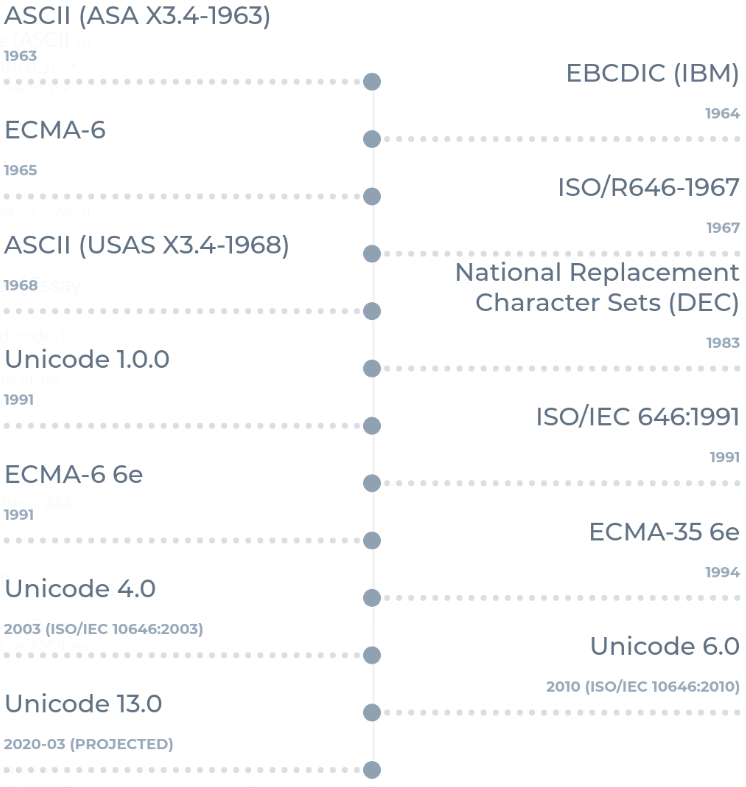
\includegraphics[width=0.5\textwidth]{media/charset-timeline.png}
\caption{Timeline of selected character sets.}
\label{fig:charset-timeline}
\end{wrapfigure}

With the high bit of an octet byte going largely unused as a parity bit, the
seven-bit character sets were rapidly expanded into a wide variety of eight-bit
character sets (sometimes mistakenly referred to as ``extended'' or ``high'' ASCII).

\textbf{FIXME FIXME}

This discordant cacophony gave rise to \textit{mojibake} (文字化け [{\fontspec{DejaVu Serif}mod͡ʑibake}]),
the garbled result of mismatched character encoding and decoding\footnote{Japanese, from 文字 (moji (character))
化ける (bakeru (take a different form)). Russians know it as \textrussian{кракозя́бры}
(krakozyabry [{\fontspec{DejaVu Serif}krɐkɐˈzʲæbrɪ̈}]) or sometimes
\textrussian{бНОПНЯ} (bnopnjá {\fontspec{DejaVu Serif}bnɐpˈnʲa}), while
Bulgarians speak of \textbulgarian{маймуница} (majmunica (monkey alphabet)).
Serbs cut to a characteristically Balkan chase with \textrussian{ђубре} (đubre
(trash)). I {\fontspec{DejaVu Serif}�} Unicode.}.

\subsection{Consilience: the Universal Character Set}
\label{sec:ucs}
\begin{table}[h]
  \begin{center}
    \begin{tabular}{ |c|p{.65\textwidth}| }
      \hline
      Principle & Statement \\
      \hline
      \hline
      Universality & The Unicode Standard provides a single, universal repertoire. \\
      \hline
      Efficiency & Unicode text is simple to parse and process. \\
      \hline
      Characters, not glyphs & The Unicode Standard encodes characters, not glyphs. \\
      \hline
      Semantics & Characters have well-defined semantics. \\
      \hline
      Plain text & Unicode characters represent plain text. \\
      \hline
      Logical order & The default for memory representation is logical order. \\
      \hline
      Unification & The Unicode Standard unifies duplicate characters within scripts across languages. \\
      \hline
      Dynamic composition & Accented forms can be dynamically composed. \\
      \hline
      Stability & Characters, once assigned, cannot be reassigned and key properties are immutable. \\
      \hline
      Convertibility & Accurate convertibility is guaranteed between the Unicode Standard and other widely accepted standards. \\
      \hline
    \end{tabular}
  \end{center}
  \caption{The 10 Design Principles of Unicode (Unicode Core Specification §2.2\cite{unicode}).}
  \label{table:ucsdesign}
\end{table}
The Universal Character Set (ISO 10646\footnote{Note that this is 10,000 more than ISO 646.},
the character set underlying Unicode) was introduced to resolve these problems,
as a ``unique, universal, and uniform character encoding''\cite{unicodehistory}. The
Unicode Consortium traces its origin to Joe Becker's paper, ``Unicode 88''\cite{unicode88}.
Often in these early documents, UCS is described as a ``16-bit character set'', and
this is partially responsible for the widespread misconception that UTF-16\cite{rfc2781}
can encode all UCS code points in a single 16-bit unit. 16 bits are sufficient
to encode any given UCS \textit{plane} of up to 65,536 code points, and a great
many languages are contained within the first UCS plane, the Basic Multilingual
Plane (0x0--0xffff). There are a total of 17 planes available in
UCS\footnote{Once upon a time, these other sixteen planes were known as the
Astral Planes\cite{astralplanes}.}, however, and UTF-16 requires two code
units to encode points from these other 16 planes (0x10000--0x10ffff).

\begin{table}[h]
  \begin{center}
    \begin{tabular}{ |c|c|p{.6\textwidth}| }
      \hline
      Plane & ID & Purpose \\
      \hline
      \hline
      Basic Multilingual & 0 & Common-use characters for modern and historical scripts. \\
      \hline
      Supplementary Multilingual & 1 & Spillover from BMP. \\
      \hline
      Supplementary Ideographic & 2 & CJK spillover from BMP. \\
      \hline
      Supplementary special-purpose & 14 & Format control spillover. \\
      \hline
      Supplementary Private Use A & 15 & Local semantics. \\
      \hline
      Supplementary Private Use B & 16 & Local semantics. \\
      \hline
    \end{tabular}
  \end{center}
  \caption{The six named UCS planes (Unicode Core Specification §2.8\cite{unicode}).}
  \label{table:ucsdesign}
\end{table}

\textbf{FIXME FIXME FIXME}

\subsection{Emoji}
\textbf{FIXME FIXME FIXME}

You might have seen what appeared to be emoji flags of the world. The Unicode
Consortium, in their wisdom, wanted nothing to do with such geopolitical
questions. Instead, the 26 ``Regional Indicator Symbols``---one for each
letter of the ISO basic Latin alphabet\cite{iso646}---can be used to encode
ISO 3166-1\cite{iso3166} two-letter country codes\cite{darkcorners}. Some fonts contain flag
glyphs, and some layout engines will map pairs of these symbols to flags. The
UCS \textit{does not} contain general ``flag emoji''.

\begin{figure}
  \centering
  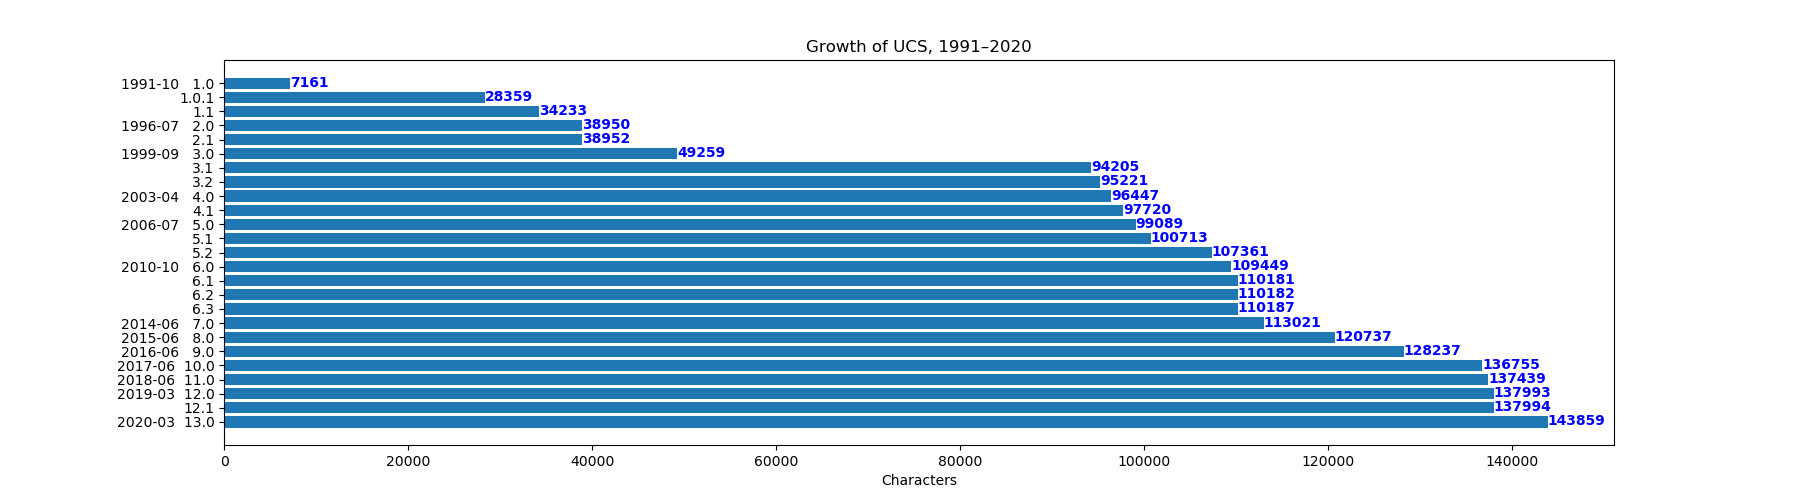
\includegraphics[width=1.1\linewidth]{media/unicode-growth.png}
  \caption{2020's Unicode 13.0 ships 143,859 character definitions.}
  \label{fig:unicodegrowth}
\end{figure}

\subsection{UTF-8}
\subsection{Stupid Unicode tricks}
\textbf{FIXME} cyclic groups, reversals, zalgo, \url{http://qaz.wtf/u/, half blocks}

\subsection{Fixed-width fonts ain't so fixed}

Notcurses assumes that all glyphs occupy widths which are an integral multiple
of the smallest possible glyph's cell width (aka a ``fixed-width font'').
Unicode introduces characters which generally occupy two such cells, known as
wide characters (though in the end, width of a glyph is a property of the
font). It is not possible to print half of such a glyph, nor is it generally
possible to print a wide glyph on the last column of a terminal.

Notcurses does not consider it an error to place a wide character on the last
column of a line. It will obliterate any content which was in that cell, but
will not itself be rendered. The default content will not be reproduced in such
a cell, either. When any character is placed atop a wide character's left or
right half, the wide character is obliterated in its entirety. When a wide
character is placed, any character under its left or right side is annihilated,
including wide characters. It is thus possible for two wide characters to sit
at columns 0 and 2, and for both to be obliterated by a single wide character
placed at column 1.

Likewise, when rendering, a plane which would partially obstruct a wide glyph
prevents it from being rendered entirely. A pathological case would be that of
a terminal $n$ columns in width, containing $n-1$ planes, each 2 columns wide.
The planes are placed at offsets $[0\ldots n-2]$. Each plane is above the plane to
its left, and each plane contains a single wide character. Were this to be
rendered, only the rightmost glyph would be rendered!

Finally, fonts and font engines which yield glyphs wider (or narrower) than
\texttt{wcwidth()} would lead Notcurses to believe can cause problems. It is
best to avoid EGCs known to be very wide, or to avoid fonts which generate very
wide glyphs. Some examples are shown in Figure~\ref{fig:wideglyphs}.

\begin{figure}
\centering
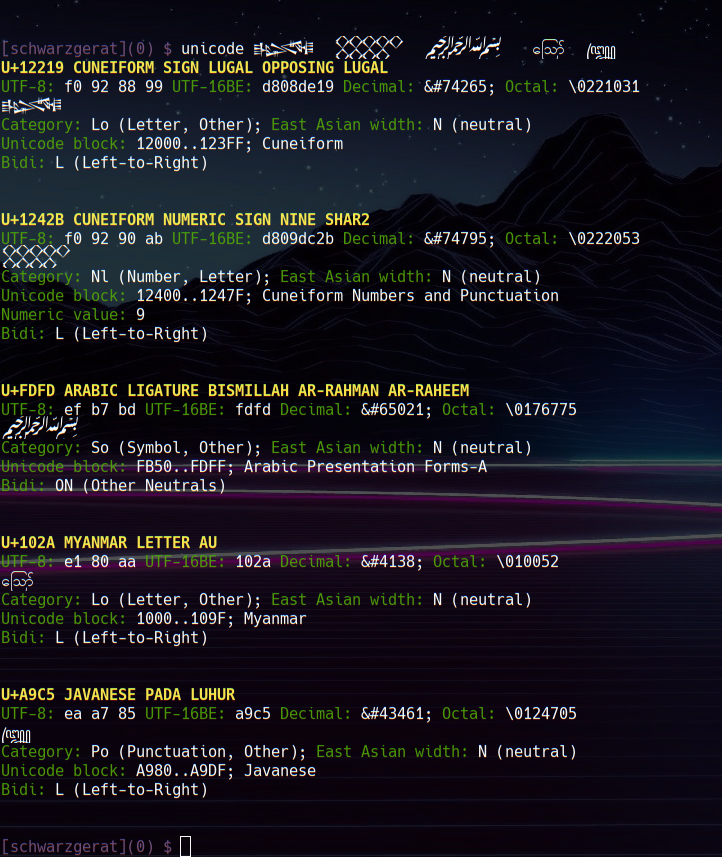
\includegraphics[width=1\linewidth]{media/wide-unicode.png}
\caption[Some very wide Unicode glyphs]{Some very wide Unicode glyphs (font: Hack 10)}
\label{fig:wideglyphs}
\end{figure}

\newpage
%%%%%%%%%%%%%%%%%%%%%%%%%%%%%%%%%%%%%%%%%%%%%%%%%%%%%%%%%%%%%%%%%%%%%%%%
\section{Using ncplanes}
\label{sec:planes}
\epigraph{Even when I say nothing,\\ it's a beautiful use of negative space.}{Company Flow,\\``The Fire in Which you Burn''}
\label{ncplane}
As mentioned in Chapter~\ref{sec:fullscreen}, \texttt{ncplane}s (henceforth
simply planes) are the fundamental drawing surface of Notcurses. A Notcurses
instance contains a z-axis on which planes are totally ordered\footnote{Future
releases of Notcurses might relax this to a partial ordering, allowing
multiple ncplanes to partition a logical level. See
\url{https://github.com/dankamongmen/notcurses/issues/184}.}. In addition, it
always contains at least one plane, the \textit{standard plane}. This plane's
origin is always defined to be the rendering area's origin. It is always
exactly as large as the rendering area, and it cannot be destroyed.

It's useful to note that there is never a \textit{need} for more than one plane,
as demonstrated by the simple fact that each rendered frame is a two-dimensional
area. Planes do not add power to the system: \textit{any algorithm which can be expressed using multiple planes can be expressed
using a single plane and external state.} Instead, they add expressiveness, and
supply order to the state needed beyond the data present in the rendered frame.
The color blending performed for transparent or translucent planes can be
simulated by the programmer. Redrawing the parts of an underlying plane exposed
by moving another can be managed by the programmer. Mapping a base glyph to
null cells of different planes can be done by keeping an index for each null
cell, etc.\ etc. In a great many cases, this external structure would be
reproducing the algorithms and data structures of planes. \textbf{Planes are
provided as a concise and efficient implementation of the codes frequently
necessary to implement TUIs}. The rule for using planes is thus simply to
\textit{use a plane whenever you find yourself implementing code already
provided by planes}.

Chapter \ref{sec:notcursesfuncs} introduced one function that creates a new
plane: \texttt{ncplane\_new()}. In addition, there is \texttt{ncplane\_aligned()}.

\begin{listing}[!htb]
\begin{minted}{C}
// Create a new ncplane at the specified 'yoff', of the specified 'rows' and 'cols'. Align this plane
// according to 'align' relative to 'n'.
struct ncplane* ncplane_aligned(struct ncplane* n, int rows, int cols, int yoff, ncalign_e align, void* opaque);
\end{minted}
\caption{Creating a new plane aligned relative to another.}
\end{listing}

A plane is defined by:
\begin{denseitemize}
\item{A packed ``framebuffer'' of \texttt{cell} structures. Cells are discussed
    in detail in~\ref{sec:cells}; it is enough now to know that each has an
    EGC, a set of attributes, and a fore- and background color.}
\item{A ``base cell'', rendered for any cell with a null EGC.}
\item{A cursor position relative to the plane's origin.}
\item{The plane's position relative to the visible area's origin.}
\item{A two-dimensional size.}
\item{An ``egcpool'' providing backing storage for the framebuffer's complex EGCs.}
\item{An opaque pointer (the \textit{user pointer}), controlled by the application.}
\item{A current set of attributes and colors.}
\item{A pointer to the plane below this one, or \texttt{NULL} for the bottommost plane.}
\end{denseitemize}

However a plane is created---including the standard plane---it is initialized
in the same way. All cells--both the base cell and those of the
framebuffer---are zeroed out. A zeroed cell has the null glyph (UTF-8
value ``00''), no attributes, and the default foreground and background color
(default colors are always opaque). Note that planes are thus by default
glyph-transparent but color-opaque. The cursor is placed at the origin. The
plane's current attributes and channels are likewise zeroed out. The plane is
pushed onto the top of the z-axis and assigned an initialized egcpool
(see~\ref{sec:egcpools}).

Besides the default plane, planes may occupy any positive size (both the number
of rows and columns must be greater than zero), and have their origins any
integer offset from the visual origin. It is possible for a plane to be a
superset of the visual area, a subset, to exactly match the visual area, to
partially overlap it, or even to be entirely off-screen. A plane can be
moved to any coordinate, but the plane's cursor cannot be moved off the plane.
\begin{listing}[!htb]
\begin{minted}{C}
// Duplicate an existing ncplane. The new plane will have the same geometry, will duplicate all content, and
// will start with the same rendering state. The new plane will be immediately above the old one on the z axis.
struct ncplane* ncplane_dup(struct ncplane* n, void* opaque);
\end{minted}
\caption{Duplicating a plane.}
\end{listing}
A plane can be duplicated with \texttt{ncplane\_dup()}. This will create a new
plane of the same geometry at the top of the z-axis. It will then have all
other properties duplicated, using its own egcpool. A new user pointer can be
provided at duplication time.
\begin{listing}[!htb]
\begin{minted}{C}
void* ncplane_set_userptr(struct ncplane* n, void* opaque);
void* ncplane_userptr(struct ncplane* n);
\end{minted}
\caption{Manipulating a plane's user pointer.}
\end{listing}
Each method of creating a plane allows a user pointer to be supplied. The plane
will never touch this pointer---it exists wholly for the benefit of the calling
program. Retrieve it with \texttt{ncplane\_userptr()}, and reset it with
\texttt{ncplane\_set\_userptr()}. The same user pointer can be held by multiple
planes, should you so desire.

\begin{listing}[!htb]
\begin{minted}{C}
// Destroy the specified ncplane. None of its contents will be visible after the next
// call to notcurses_render(). It is an error to attempt to destroy the standard plane.
int ncplane_destroy(struct ncplane* ncp);

// Destroy all ncplanes other than the standard plane.
void notcurses_drop_planes(struct notcurses* nc);
\end{minted}
\caption{Destroying planes.}
\end{listing}
Any plane save the standard plane may be destroyed with \texttt{ncplane\_destroy()}.
All planes save the standard plane may be destroyed in one fell swoop with
\texttt{notcurses\_drop\_planes()}.

\subsection{Moving and resizing planes}
\begin{listing}[!htb]
\begin{minted}{C}
// Splice ncplane 'n' out of the z-buffer, and reinsert it at the top or bottom.
int ncplane_move_top(struct ncplane* n);
int ncplane_move_bottom(struct ncplane* n);

// Splice ncplane 'n' out of the z-buffer, and reinsert it above/below 'targ'.
int ncplane_move_above_unsafe(struct ncplane* restrict n, struct ncplane* restrict targ);
int ncplane_move_below_unsafe(struct ncplane* restrict n, struct ncplane* restrict targ);

static inline int ncplane_move_above(struct ncplane* n, struct ncplane* above){
  if(n == above){
    return -1;
  }
  return ncplane_move_above_unsafe(n, above);
}

static inline int ncplane_move_below(struct ncplane* n, struct ncplane* below){
  if(n == below){
    return -1;
  }
  return ncplane_move_below_unsafe(n, below);
}

// Return the plane below this one, or NULL if this is at the bottom.
struct ncplane* ncplane_below(struct ncplane* n);
\end{minted}
\caption{Moving planes on the z axis.}
\label{listing:zaxismoves}
\end{listing}
Even the standard plane can be reordered along the z-axis (Listing~\ref{listing:zaxismoves}).
\texttt{ncplane\_move\_top()} and \texttt{ncplane\_move\_bottom()} are absolute, moving the specified plane
to the top or bottom of the z-axis, respectively. \texttt{ncplane\_move\_above()}
and \texttt{ncplane\_move\_below()} are relative, moving the plane immediately
above or below another one. It is an error to try and move a plane below or above itself,
or above or below \texttt{NULL}. Likewise, an error will be returned if the relative
plane does not exist on the z-axis.
\begin{listing}[!htb]
\begin{minted}{C}
// Move this plane relative to the standard plane. It is an error to attempt to move the standard plane.
int ncplane_move_yx(struct ncplane* n, int y, int x);
\end{minted}
\caption{Moving planes on the x and y axis.}
\label{list:xyaxismoves}
\end{listing}
All planes other than the standard plane can be moved in the x- and y-dimensions. It is permitted to move
a plane partially or even entirely outside of the viewing area. A plane which
lies entirely outside the rendering window plays no role in the rendering
process.
\begin{listing}[!htb]
\begin{minted}{C}
int ncplane_resize(struct ncplane* n, int keepy, int keepx, int keepleny,
                   int keeplenx, int yoff, int xoff, int ylen, int xlen);

static inline int ncplane_resize_simple(struct ncplane* n, int ylen, int xlen){
  int oldy, oldx;
  ncplane_dim_yx(n, &oldy, &oldx); // current dimensions of 'n'
  int keepleny = oldy > ylen ? ylen : oldy;
  int keeplenx = oldx > xlen ? xlen : oldx;
  return ncplane_resize(n, 0, 0, keepleny, keeplenx, 0, 0, ylen, xlen);
}
\end{minted}
\caption{Resizing a plane can retain any amount of the old material.}
\label{list:planeresize}
\end{listing}
All planes other than the standard plane can be resized (Listing~\ref{list:planeresize}).
Resizing is a very general and powerful operation---it is possible to implement
\texttt{ncplane\_move\_yx()} in terms of \texttt{ncplane\_resize()}. The four
parameters \texttt{keepy}, \texttt{keepx}, \texttt{keepleny}, and
\texttt{keeplenx} define a subset of the plane to retain. The retained
rectangle has its origin at \texttt{keepy},\texttt{keepx}, and a
\texttt{keepleny}-row, \texttt{keeplenx}-column geometry. If either of the
dimensions are zero, no material is retained. In this case, \texttt{keepx} and
\texttt{keepy} are immaterial, save that in no case may any of these four
parameters be negative. \texttt{keepx} and \texttt{keepy} are both relative to
the plane's origins, \textit{not} the rendering area. Attempting to ``retain''
material beyond the boundaries of the plane is an error. \texttt{yoff} and
\texttt{xoff} are likewise relative to the plane's origin, and define the
geometry of the plane following the resize. Both of these arguments must be
positive. Attempting to retain more material than there is room in the reshaped
plane is an error.

Yeah, that's a little complex. \texttt{ncplane\_resize\_simple()} is provided
as a gentler path to resizing. It retains everything it can (everything, if no
shrinking is going on), preferring material towards the upper left. The resulting
plane does not move from its origin.
\begin{listing}[!htb]
\begin{minted}{C}
// provided a coordinate relative to the origin of 'src', map it to the same absolute coordinate
// relative to thte origin of 'dst'. either or both of 'y' and 'x' may be NULL.
void ncplane_translate(const struct ncplane* src, const struct ncplane* dst, int* restrict y, int* restrict x);

// Fed absolute 'y'/'x' coordinates, determine whether that coordinate is within the ncplane 'n'. If not, return false.
// If so, return true. Either way, translate the absolute coordinates relative to 'n'. If the point is not within 'n',
// these coordinates will not be within the dimensions of the plane.
bool ncplane_translate_abs(const struct ncplane* n, int* restrict y, int* restrict x);
\end{minted}
\caption{Translating coordinates between planes.}
\label{list:translateplanes}
\end{listing}
Sometimes it is useful to translate coordinates between planes
(Listing~\ref{list:translateplanes}), or between the visible area and planes
(this latter is particularly useful when interpreting mouse clicks; see
Chapter~\ref{sec:input}).
\begin{listing}[!htb]
\begin{minted}{C}
int ncplane_at_cursor(struct ncplane* n, cell* c);
int ncplane_at_yx(struct ncplane* n, int y, int x, cell* c);
\end{minted}
\caption{Reflecting on the plane to acquire its contents.}
\label{listing:planereflect}
\end{listing}
The content of a plane can be retrieved using reflection (Listing~\ref{listing:planereflect}).
Any coordinate relative to the plane's origin can be provided, along with a
value-result \texttt{cell} structure. If the coordinates are valid for the
plane, the cell at those coordinates will be copied into \texttt{c}, and the
number of bytes required to store its EGC will be returned. A value less than
zero is returned on error.


Just as each cell has a set of attributes and channels, the plane itself has
an active attribute set and active channels. These can be freely manipulated
using the API of Listings~\ref{listing:planeraw}, \ref{listing:planefg}, \ref{listing:planebg}, and
\ref{listing:planeattr}.

\begin{listing}[!htb]
\begin{minted}{C}
// get the current channels or attribute word for ncplane 'n'.
uint64_t ncplane_channels(const struct ncplane* n);
uint32_t ncplane_attr(const struct ncplane* n);
\end{minted}
\caption{Accessing a plane's raw channels and attributes.}
\label{listing:planeraw}
\end{listing}

\begin{listing}[!htb]
\begin{minted}{C}
// Extract the 32-bit working foreground channel from an ncplane.
static inline unsigned ncplane_fchannel(const struct ncplane* nc){
  return channels_fchannel(ncplane_channels(nc));
}

// Extract 24 bits of working foreground RGB from an ncplane, shifted to LSBs.
static inline unsigned ncplane_fg(const struct ncplane* nc){
  return channels_fg(ncplane_channels(nc));
}

// Extract 2 bits of foreground alpha from 'struct ncplane', shifted to LSBs.
static inline unsigned ncplane_fg_alpha(const struct ncplane* nc){
  return channels_fg_alpha(ncplane_channels(nc));
}

// Extract 24 bits of foreground RGB from 'n', split into subcomponents.
static inline unsigned ncplane_fg_rgb(const struct ncplane* n, unsigned* r, unsigned* g, unsigned* b){
  return channels_fg_rgb(ncplane_channels(n), r, g, b);
}

// Set the current fore/background color using RGB specifications. If the terminal does not support
// directly-specified 3x8b cells (24-bit "TrueColor", indicated by the "RGB" terminfo capability),
// the provided values will be interpreted in some lossy fashion. None of r, g, or b may exceed 255.
// "HP-like" terminals require setting foreground and background at the same time using "color pairs";
// notcurses will manage color pairs transparently.
int ncplane_set_fg_rgb(struct ncplane* n, int r, int g, int b);

// Same, but clipped to [0..255].
void ncplane_set_fg_rgb_clipped(struct ncplane* n, int r, int g, int b);

// Same, but with rgb assembled into a channel (i.e. lower 24 bits).
int ncplane_set_fg(struct ncplane* n, unsigned channel);

// Use the default color for the foreground/background.
void ncplane_set_fg_default(struct ncplane* n);

// Set the ncplane's foreground palette index, set the foreground palette index bit, set it
// foreground-opaque, and clear the foreground default color bit.
int ncplane_set_fg_palindex(struct ncplane* n, int idx);

// Set the alpha parameters for ncplane 'n'.
int ncplane_set_fg_alpha(struct ncplane* n, int alpha);
\end{minted}
\caption{Manipulating a plane's active foreground channel.}
\label{listing:planefg}
\end{listing}

\begin{listing}[!htb]
\begin{minted}{C}
// Extract the 32-bit working background channel from an ncplane.
static inline unsigned ncplane_bchannel(const struct ncplane* nc){
  return channels_bchannel(ncplane_channels(nc));
}

// Extract 24 bits of working background RGB from an ncplane, shifted to LSBs.
static inline unsigned ncplane_bg(const struct ncplane* nc){
  return channels_bg(ncplane_channels(nc));
}

// Extract 2 bits of background alpha from 'struct ncplane', shifted to LSBs.
static inline unsigned ncplane_bg_alpha(const struct ncplane* nc){
  return channels_bg_alpha(ncplane_channels(nc));
}

// Extract 24 bits of background RGB from 'n', split into subcomponents.
static inline unsigned ncplane_bg_rgb(const struct ncplane* n, unsigned* r, unsigned* g, unsigned* b){
  return channels_bg_rgb(ncplane_channels(n), r, g, b);
}

int ncplane_set_bg_rgb(struct ncplane* n, int r, int g, int b);
void ncplane_set_bg_rgb_clipped(struct ncplane* n, int r, int g, int b);
int ncplane_set_bg(struct ncplane* n, unsigned channel);
void ncplane_set_bg_default(struct ncplane* n);
int ncplane_set_bg_palindex(struct ncplane* n, int idx);
int ncplane_set_bg_alpha(struct ncplane* n, int alpha);
\end{minted}
\caption{Manipulating a plane's active background channel.}
\label{listing:planebg}
\end{listing}

\begin{listing}[!htb]
\begin{minted}{C}
// Set the specified style bits for the ncplane 'n', whether they're actively supported or not.
void ncplane_styles_set(struct ncplane* n, unsigned stylebits);

// Add the specified styles to the ncplane's existing spec.
void ncplane_styles_on(struct ncplane* n, unsigned stylebits);

// Remove the specified styles from the ncplane's existing spec.
void ncplane_styles_off(struct ncplane* n, unsigned stylebits);

// Return the current styling for this ncplane.
unsigned ncplane_styles(const struct ncplane* n);
\end{minted}
\caption{Manipulating a plane's active attributes.}
\label{listing:planeattr}
\end{listing}

During the course of \texttt{notcurses\_render()}, the plane is examined at
all cells intersecting with unsolved coordinates (see~\ref{sec:rendering}).
Whenever the EGC at a cell is the null EGC (a \texttt{gcluster} value of 0;
recall that this is the default value), the plane's base cell is instead
considered for rendering purposes. This applies to glyph, attribute, and
colors---there is not yet any means to make multiple cells in a plane glyph-transparent
with different colors\footnote{See \url{https://github.com/dankamongmen/notcurses/issues/395}.}.

\begin{listing}[!htb]
\begin{minted}{C}
// Set the ncplane's base cell to this cell. It will be used for purposes of rendering anywhere that the ncplane's
// gcluster is 0. Erasing the ncplane does not reset the base cell; this function must be called with a zero 'c'.
int ncplane_set_base_cell(struct ncplane* ncp, const cell* c);

// Set the ncplane's base cell to this cell. It will be used for purposes of rendering anywhere that the ncplane's
// gcluster is 0. Erasing the ncplane does not reset the base cell; this function must be called with an empty
// 'egc'. 'egc' must be a single extended grapheme cluster.
int ncplane_set_base(struct ncplane* ncp, uint64_t channels, uint32_t attrword, const char* egc);

// Extract the ncplane's base cell into 'c'. The reference is invalidated if 'ncp' is destroyed.
int ncplane_base(struct ncplane* ncp, cell* c);
\end{minted}
\caption{Manipulating a plane's base cell.}
\end{listing}

\begin{listing}[!htb]
\begin{minted}{C}
// Alignment within the ncplane. Left/right-justified, or centered.
typedef enum { NCALIGN_LEFT, NCALIGN_CENTER, NCALIGN_RIGHT, } ncalign_e;

// Return the column at which 'c' cols ought start in order to be aligned according to 'align' within ncplane 'n'.
// Returns INT_MAX on invalid 'align'. Undefined behavior on negative 'c'.
static inline int ncplane_align(const struct ncplane* n, ncalign_e align, int c){
  if(align == NCALIGN_LEFT){
    return 0;
  }
  int cols = ncplane_dim_x(n);
  if(align == NCALIGN_CENTER){
    return (cols - c) / 2;
  }else if(align == NCALIGN_RIGHT){
    return cols - c;
  }
  return INT_MAX;
}
\end{minted}
\caption{Aligning output within a plane.}
\end{listing}

\begin{listing}[!htb]
\begin{minted}{C}
int ncplane_rotate_cw(struct ncplane* n);
int ncplane_rotate_ccw(struct ncplane* n);
\end{minted}
\caption{Aligning output within a plane.}
\label{listing:rotate}
\end{listing}
It's possible in rather limited circumstances to perform a rotation of a plane
(Listing~\ref{listing:rotate}). This only really works for planes entirely
populated by half blocks or characters which can be composed from half blocks.
The plane is rotated by $\frac{\pi}{2}$ radians in either direction. Note that
the rotation is only lossless in terms of color and geometry; it is possible
for half blocks to be rotated into full blocks, and vice versa. You are
encouraged to consult the source code before making use of rotations.

\subsection{Cells}
\label{sec:cells}
Each coordinate of an plane corresponds to a \texttt{cell}. The cell definition
is exposed to the application, though it should not generally be directly
manipulated. A multicolumn cell (a cell containing an EGC of $n$ columns where
$n>1$) overrides the $n-1$ following cells. Since there are always a fixed
number of cells, this means that the overridden cells are skipped during
rendering, as well as being zeroed out at the time the multicolumn EGC is
written to the cell.
\begin{listing}[!htb]
\begin{minted}{C}
typedef struct cell {
  // These 32 bits are either a single-byte, single-character grapheme cluster (values 0–0x7f), or
  // an offset into a per-ncplane attached pool of varying-length UTF-8 grapheme clusters.
  uint32_t gcluster;          // 4B -> 4B
  uint32_t attrword;          // + 4B -> 8B
  uint64_t channels;          // + 8B == 16B
} cell;
\end{minted}
\caption{The \texttt{cell} definition.}
\end{listing}
The \texttt{gcluster} field is a 32-bit number. If the value is less than 128,
it directly specifies its UTF-8 encoded character. Since Unicode's first 128
values are taken directly from ASCII, this means the entirety of ASCII can be
represented in-line. If the value is greater than or equal to 128, it is a
bias-128 index into the plane's associated egcpool. Since egcpools are per-plane,
this implies that it is unsafe to blindly copy a cell from one plane to another.

Applications generally need not work directly with cells, though sometimes it
is easiest to do so. The usual reason for working with a cell is either to set
all three properies of output at once (glyph, attributes, and colors), or to
receive all three properties at once when retrieving a coordinate's data.

As further discussed in Chapter~\ref{sec:channels}, the \texttt{channels}
variable is a 64-bit field packing together a number of properties. The high
32 bits apply to the foreground, and the low 32 bits to the background. They
can be set and queried as a channel (Listing~\ref{listing:cellchannels}).

\begin{listing}[!htb]
\begin{minted}{C}
// Extract the 32-bit background channel from a cell.
static inline unsigned cell_bchannel(const cell* cl){
  return channels_bchannel(cl->channels);
}

// Extract the 32-bit foreground channel from a cell.
static inline unsigned cell_fchannel(const cell* cl){
  return channels_fchannel(cl->channels);
}

// Set the 32-bit background channel of a cell.
static inline uint64_t cell_set_bchannel(cell* cl, uint32_t channel){
  return channels_set_bchannel(&cl->channels, channel);
}

// Set the 32-bit foreground channel of a cell.
static inline uint64_t cell_set_fchannel(cell* cl, uint32_t channel){
  return channels_set_fchannel(&cl->channels, channel);
}
\end{minted}
\caption{Modifying \texttt{cell} channels.}
\label{listing:cellchannels}
\end{listing}

RGB values consume 24 bits of each channel, 75\% of the 64 bits in \texttt{channels}.
RGB values can be blended, clipped, and otherwise dealt with arithmetically.

\begin{listing}[!htb]
\begin{minted}{C}
// do not pass palette-indexed channels!
static inline uint64_t cell_blend_fchannel(cell* cl, unsigned channel, unsigned* blends){
  return cell_set_fchannel(cl, channels_blend(cell_fchannel(cl), channel, blends));
}

// Extract 24 bits of foreground RGB from 'cell', shifted to LSBs.
static inline unsigned cell_fg(const cell* cl){
  return channels_fg(cl->channels);
}

// Extract 2 bits of foreground alpha from 'cell', shifted to LSBs.
static inline unsigned cell_fg_alpha(const cell* cl){
  return channels_fg_alpha(cl->channels);
}

// Extract 24 bits of foreground RGB from 'cell', split into components.
static inline unsigned cell_fg_rgb(const cell* cl, unsigned* r, unsigned* g, unsigned* b){
  return channels_fg_rgb(cl->channels, r, g, b);
}

// Set the r, g, and b cell for the foreground component of this 64-bit
// 'cell' variable, and mark it as not using the default color.
static inline int cell_set_fg_rgb(cell* cl, int r, int g, int b){
  return channels_set_fg_rgb(&cl->channels, r, g, b);
}

// Same, but clipped to [0..255].
static inline void cell_set_fg_rgb_clipped(cell* cl, int r, int g, int b){
  channels_set_fg_rgb_clipped(&cl->channels, r, g, b);
}

// Same, but with an assembled 24-bit RGB value.
static inline int cell_set_fg(cell* c, uint32_t channel){
  return channels_set_fg(&c->channels, channel);
}
\end{minted}
\caption{\texttt{cell} foreground RGBA functionality.}
\label{listing:cellrgbfg}
\end{listing}

\begin{listing}[!htb]
\begin{minted}{C}
static inline uint64_t cell_blend_bchannel(cell* cl, unsigned channel, unsigned* blends){
  return cell_set_bchannel(cl, channels_blend(cell_bchannel(cl), channel, blends));
}

// Extract 24 bits of background RGB from 'cell', shifted to LSBs.
static inline unsigned cell_bg(const cell* cl){
  return channels_bg(cl->channels);
}

// Extract 2 bits of background alpha from 'cell', shifted to LSBs.
static inline unsigned cell_bg_alpha(const cell* cl){
  return channels_bg_alpha(cl->channels);
}

// Extract 24 bits of background RGB from 'cell', split into components.
static inline unsigned cell_bg_rgb(const cell* cl, unsigned* r, unsigned* g, unsigned* b){
  return channels_bg_rgb(cl->channels, r, g, b);
}

// Set the r, g, and b cell for the background component of this 64-bit
// 'cell' variable, and mark it as not using the default color.
static inline int cell_set_bg_rgb(cell* cl, int r, int g, int b){
  return channels_set_bg_rgb(&cl->channels, r, g, b);
}

// Same, but clipped to [0..255].
static inline void cell_set_bg_rgb_clipped(cell* cl, int r, int g, int b){
  channels_set_bg_rgb_clipped(&cl->channels, r, g, b);
}

// Same, but with an assembled 24-bit RGB value.
static inline int cell_set_bg(cell* c, uint32_t channel){
  return channels_set_bg(&c->channels, channel);
}
\end{minted}
\caption{\texttt{cell} background RGBA functionality.}
\label{listing:cellrgbbg}
\end{listing}

It is also possible to make use of palette-indexed color (recall that the size
of the palette can be acquired with \texttt{notcurses\_palette\_size()}).
Palette-indexed color requires much less bandwidth than pure RGB (indeed, work
is underway to emit palette-indexed rasterization even when RGB has been
provided---see \url{https://github.com/dankamongmen/notcurses/issues/371}),
and allows for finer control on terminals which don't faithfully implement RGB
TrueColor. The terminal palette can be manually reprogrammed with the
palette256 API (see Chapter~\ref{list:palette256}).

\begin{listing}[!htb]
\begin{minted}{C}
// Set the cell's foreground palette index, set the foreground palette index
// bit, set it foreground-opaque, and clear the foreground default color bit.
static inline int cell_set_fg_palindex(cell* cl, int idx){
  if(idx < 0 || idx >= NCPALETTESIZE){
    return -1;
  }
  cl->channels |= CELL_FGDEFAULT_MASK;
  cl->channels |= CELL_FG_PALETTE;
  cl->channels &= ~(CELL_ALPHA_MASK << 32u);
  cl->attrword &= 0xffff00ff;
  cl->attrword |= (idx << 8u);
  return 0;
}

static inline unsigned cell_fg_palindex(const cell* cl){
  return (cl->attrword & 0x0000ff00) >> 8u;
}

// Set the cell's background palette index, set the background palette index
// bit, set it background-opaque, and clear the background default color bit.
static inline int cell_set_bg_palindex(cell* cl, int idx){
  if(idx < 0 || idx >= NCPALETTESIZE){
    return -1;
  }
  cl->channels |= CELL_BGDEFAULT_MASK;
  cl->channels |= CELL_BG_PALETTE;
  cl->channels &= ~CELL_ALPHA_MASK;
  cl->attrword &= 0xffffff00;
  cl->attrword |= idx;
  return 0;
}

static inline unsigned cell_bg_palindex(const cell* cl){
  return cl->attrword & 0x000000ff;
}

static inline bool cell_fg_palindex_p(const cell* cl){
  return channels_fg_palindex_p(cl->channels);
}

static inline bool cell_bg_palindex_p(const cell* cl){
  return channels_bg_palindex_p(cl->channels);
}
\end{minted}
\caption{\texttt{cell} palette-indexed color functionality.}
\label{listing:cellpalette}
\end{listing}

Finally, the default fore- and/or background color can be used, and is indeed
the default. Default colors can't be blended. Some terminals can be configured
to use a transparent background. Only in cells using the default background
color can this effect be seen.

\begin{listing}[!htb]
\begin{minted}{C}
// Is the background using the "default background color"? The "default background color"
// must generally be used to take advantage of terminal-effected transparency.
static inline bool cell_bg_default_p(const cell* cl){
  return channels_bg_default_p(cl->channels);
}

// Is the foreground using the "default foreground color"?
static inline bool cell_fg_default_p(const cell* cl){
  return channels_fg_default_p(cl->channels);
}
\end{minted}
\caption{\texttt{cell} default color functionality.}
\end{listing}

\subsection{egcpools}
\label{sec:egcpools}
Each plane is backed by an \texttt{egcpool} structure. Any cell requiring more
than a single byte to encode its EGC will write the EGC to the egcpool, and
store a byte-granular index into the actual \texttt{gcluster} field of the
\texttt{cell}. The first 128 UTF-8 characters are stored directly, and thus
any \texttt{gcluster} value greater than or equal to 128 is actually a
biased\footnote{128-biased, i.e. \texttt{gcluster} is the offset + 128.}
index into the pool. The pool can grow as large as $2^{25}$ bytes (32 MiB).
Each EGC is stored as a NUL-terminated string, so the minimum size is three
bytes (since all single-byte UTF-8 is inlined, the minimum UTF-8 EGC to be
placed in the pool is two bytes, plus a NUL byte).

You shouldn't ever need to work directly with egcpools, and their API is not
exposed. It is possible to exhaust an egcpool, but not without either a tremendous
geometry (start worrying around 1024x1024 or so), or a plenitude of pathological
EGCs. Should this unhappy situation occur, functions like \texttt{ncplane\_putegc()}
and even \texttt{cell\_load()} will start failing (they should not crash or otherwise
fault). There's not much you can do at this point save erase or destroy the plane\footnote{This
ought be addressed by \url{https://github.com/dankamongmen/notcurses/issues/425}.}.
Outside of deliberate attempts to trigger it during testing, I have never seen
this failure case.

\subsection{Alpha blending and plane transparency}
\label{sec:alpha}
The rendering algorithm described in Chapter~\ref{sec:rendering} is responsible
for the blending of colors and selection of glyphs from among planes. Let's look
at it in full detail.

There are three largely independent dimensions for each rendered cell, and they
are the same three dimensions of any \texttt{cell}: EGC plus attribute, foreground
color, and background color. There are three different ways that colors can be
set in the actual terminal (assuming support):

\begin{denseitemize}
\item{The ``default foreground`` and ``default background`` colors. These are
    inherited from the terminal, where they are usually user-configurable.
    Since most of the user's shell experience will take place in these colors,
    you can safely assume that either there is a high contrast difference
    between the two, or the user doesn't care much about contrast. Other than
    that, it is not safe to assume that the default background is black, white,
    blue, or even monochromatic---most terminal emulators allow an image to be
    set as the background (in which case the ``default background`` color can
    be considered translucent atop this opaque background), or even a (perhaps
    partially) transparent background (the ``default background`` color is
    translucent atop the composited desktop)\footnote{I can only speak for myself, as a Solarized-on-black enthusiast, but a
    program which forces a largely white background on a fullscreen application
    annoys the hell out of me. Try to respect the user's configured background
    where possible.}. The ``op'' terminfo capability resets
    both channels, requiring the other channel (assuming it to \textit{not} be
    the default) to be emitted even if it would normally have been elided.}
\item{Palette-indexed color. The size of the palette (usually 1, 2, 8, 16, 88,
    or 256) is indicated by the \texttt{colors} terminfo capability\footnote{A
    bad \texttt{TERM} setting will wreck havoc on colors.}. If the
    \texttt{ccc} or \texttt{initp} terminfo capabilities are present, the palette
    can be modified.}
\item{RGB color. 24 bits as 3 channels of 8 bits each are directly specified. Support
    is indicated by the terminfo \texttt{rgb} capability, or by a user-supplied
    \texttt{COLORTERM} environment variable having the value ``24bit'' or ``truecolor''.}
\end{denseitemize}

Currently, only RGB can be blended. When rendering, recall that a color dimension
is ``solved'' when the computed cell reaches ``CELL\_ALPHA\_OPAQUE'' in that channel.
The channel is initialized to ``CELL\_ALPHA\_TRANSPARENT''. What is done at each
intersecting cell depends on the computed alpha thus far; see Table~\ref{table:alphablend}.

\begin{table}[!htb]
  \begin{tabular}{|l|l|l|l|l|}
    \hline
    Alpha / Blendcount & Mode & In-alpha & In-mode & Result \\
    \hline
    \hline
    \texttt{CELL\_ALPHA\_TRANSPARENT}/0 & any & \texttt{CELL\_ALPHA\_TRANSPARENT} & any & No change \\
    \hline
    \texttt{CELL\_ALPHA\_TRANSPARENT}/0 & any & \makecell{\texttt{CELL\_ALPHA\_BLEND} or\\ \texttt{CELL\_ALPHA\_OPAQUE}} & any & \makecell{State ← Incoming\\ Blendcount ← 1} \\
    \hline
    \texttt{CELL\_ALPHA\_BLEND}/$n$ & RGB & \texttt{CELL\_ALPHA\_TRANSPARENT} & any & No change \\
    \hline
    \texttt{CELL\_ALPHA\_BLEND}/$n$ & RGB & any & Default/palette & No change \\
    \hline
    \texttt{CELL\_ALPHA\_BLEND}/$n$ & RGB & \texttt{CELL\_ALPHA\_BLEND} & RGB & \makecell{Blend\\ ++Blendcount}\\
    \hline
    \texttt{CELL\_ALPHA\_BLEND}/$n$ & RGB & \texttt{CELL\_ALPHA\_OPAQUE} & RGB & \makecell{Blend\\ mode ← \texttt{OPAQUE}\\ ++Blendcount}\\
    \hline
    \texttt{CELL\_ALPHA\_OPAQUE}/$n$ & any & any & any & No change \\
    \hline
  \end{tabular}
  \caption[Transition matrix for alpha blending.]{Transition matrix for alpha blending. On the foreground channel, encountering
    \texttt{CELL\_ALPHA\_HIGHCONTRAST} sets a bit, and then behaves as if it had been \texttt{CELL\_ALPHA\_OPAQUE}.
    Upon solving the cell, if the highcontrast bit is set, either white or black is blended into the foreground as
    necessary until a minimum contrast level is reached vis-à-vis the background.}
  \label{table:alphablend}
\end{table}


\subsection{Manual palette-indexed color}
\label{sec:palettes}
While it shouldn't ever be necessary, some algorithms are more easily expressed
using palette-indexed color. Functions for manually manipulating the palette
are available when supported by the terminal (as advertised by the ``ccc''
terminfo capability). The palette is simply an integer-indexed set of RGB values,
where those RGB values are maintained by the terminal. It is possible to change
them, in which case any output expressed with that palette index will be updated
to reflect the change. The API for manipulating the palette is provided in
Listing~\ref{list:palette256}.
\begin{listing}[!htb]
\begin{minted}{C}

typedef struct palette256 {
  uint32_t chans[NCPALETTESIZE]; // We store the RGB values as a regular ol' channel
} palette256;

// Create a new palette store. It will be initialized with notcurses's best
// knowledge of the currently configured palette.
palette256* palette256_new(struct notcurses* nc);

// Attempt to configure the terminal with the provided palette 'p'. Does not
// transfer ownership of 'p'; palette256_free() can still be called.
int palette256_use(struct notcurses* nc, const palette256* p);

// Manipulate entries in the palette store 'p'. These are *not* locked.
static inline int palette256_set_rgb(palette256* p, int idx, int r, int g, int b){
  if(idx < 0 || (size_t)idx > sizeof(p->chans) / sizeof(*p->chans)){
    return -1;
  }
  return channel_set_rgb(&p->chans[idx], r, g, b);
}

static inline int palette256_set(palette256* p, int idx, unsigned rgb){
  if(idx < 0 || (size_t)idx > sizeof(p->chans) / sizeof(*p->chans)){
    return -1;
  }
  return channel_set(&p->chans[idx], rgb);
}

static inline int palette256_get_rgb(const palette256* p, int idx, unsigned* restrict r,
                                     unsigned* restrict g, unsigned* restrict b);
  if(idx < 0 || (size_t)idx > sizeof(p->chans) / sizeof(*p->chans)){
    return -1;
  }
  return channel_rgb(p->chans[idx], r, g, b);
}

// Free the palette store 'p'.
void palette256_free(palette256* p);

// Convert the plane's content to greyscale.
void ncplane_greyscale(struct ncplane* n);
\end{minted}
\caption{The palette256 API facilitates manual palette programming.}
\label{list:palette256}
\end{listing}

\subsection{Fading and pulsing planes}
When we speak of palettes, one thing comes to mind: blingful palette fades.
Back in my misspent adolescence, this was basically the ``Hello World'' of
x86 assembly. Whip it into MCGA mode 13h, load up 0xa000, and drive those
64KB. But I reminisce\textellipsis fades are available at the plane level,
as is pulsing (a periodic fade); see Listing~\ref{list:fades}. Ironically,
this only works for RGB data at the moment, but that is a temporary restriction.

\begin{listing}[!htb]
\begin{minted}{C}
// Fade the ncplane out over the provided time, calling the specified function when done. Requires a terminal
// which supports truecolor, or at least palette modification (if the terminal uses a palette, our ability to
// fade planes is limited, and affected by the complexity of the rest of the screen). It is not safe to
// resize or destroy the plane during the fadeout.
int ncplane_fadeout(struct ncplane* n, const struct timespec* ts, fadecb fader, void* curry);

// Fade the ncplane in over the specified time. Load the ncplane with the target cells without rendering, then
// call this function. When it's done, the ncplane will have reached the target levels, starting from zeroes.
int ncplane_fadein(struct ncplane* n, const struct timespec* ts, fadecb fader, void* curry);

// Pulse the plane in and out until the callback returns non-zero, relying on the callback 'fader' to initiate
// rendering. 'ts' defines the half-period (i.e. the transition from black to full brightness, or back again).
// Proper use involves preparing (but not rendering) an ncplane, then calling ncplane_pulse(), which will fade
// in from black to the specified colors.
int ncplane_pulse(struct ncplane* n, const struct timespec* ts, fadecb fader, void* curry);
\end{minted}
\caption{Palette fades.}
\label{list:fades}
\end{listing}

The pulsing and fading functions all accept an optional callback of type
\texttt{fadecb} (Listing~\ref{list:fadecb}). If \texttt{NULL} is provided as
the callback, the functions will call \texttt{notcurses\_render()} in the
callback's place. Otherwise, the callback is provided the root
\texttt{notcurses} struct, the plane of operation, and a user-provided,
per-operation curry. If the callback does not itself call
\texttt{notcurses\_render()}, this frame of the fade will not be rendered.

\begin{listing}[!htb]
\begin{minted}{C}
// Called for each delta performed in a fade on ncp. If anything but 0 is returned, the fading operation ceases
// immediately, and that value is propagated out. If provided and not NULL, the faders will not themselves call
// notcurses_render().
typedef int (*fadecb)(struct notcurses* nc, struct ncplane* ncp, void* curry);
\end{minted}
\caption{Callback type for pulsing and fading.}
\label{list:fadecb}
\end{listing}


\newpage

%%%%%%%%%%%%%%%%%%%%%%%%%%%%%%%%%%%%%%%%%%%%%%%%%%%%%%%%%%%%%%%%%%%%%%%%
% output and styling
\section{Writing and styling text}
\label{sec:output}
\epigraph{My pad and my pen\\(ah ah, you didn't go there)!}{A Tribe Called Quest,\\``Pad and Pen''}
The most fundamental aspect of textual interfaces is, after all, text. All
valid UTF-8 can be written to a plane. If scrolling has been enabled for a
plane, any amount of text can be written. If scrolling has not been enabled,
output can only be generated through the end of the current line. All text
output functions return the number of screen columns written as their primary
return value (or a negative number on failure), and load the number of bytes
written into an auxiliary value-result parameter. If the supplied output would
exceed the line, a short number of columns will be returned. Scrolling is
disabled by default on the standard plane, and on all new planes.

\begin{listing}[!htb]
\begin{minted}{C}
// Move the cursor to the specified position (the cursor needn't be visible). Returns -1 on error,
// including negative parameters, or ones exceeding the plane's dimensions.
int ncplane_cursor_move_yx(struct ncplane* n, int y, int x);

// Get the current position of the cursor within n. y and/or x may be NULL.
void ncplane_cursor_yx(const struct ncplane* n, int* restrict y, int* restrict x);
\end{minted}
\caption{Cursor management. Each plane has its own cursor.}
\label{list:cursor}
\end{listing}

The cursor is advanced appropriately to the cell just beyond the output. If the
entire line was written, and scrolling is not enabled, the cursor will be
off-plane and must be repositioned before writing any further. If scrolling is
enabled, the cursor will either move to the first column of the next line, or
if the cursor is on the last line, the plane will be scrolled by one line (and
the cursor will move to the first column). If there is an error following some
output, the cursor will be positioned following the generated output. Comparing
the new cursor location to the old can thus reveal the amount of output generated
in the event of a failure.

To check that there was no failure, then, verify that the return value is not
negative. The entirety of the input was written if any of the following is
true:

\begin{denseitemize}
\item{The return value is equal to the number of columns required to represent the input.
    \texttt{mbswidth()}(Listing ~\ref{list:mbswidth}) can be used to find the number of columns required by
    the input.}
\item{The number of bytes written is equal to the number of bytes supplied. Since Notcurses
   supports only ASCII, \texttt{strlen()} can be used to find the number of
   bytes supplied.}
\item{The cursor is not beyond the end of the plane, and scrolling is disabled
 on the plane.}
\end{denseitemize}

\begin{listing}[!htb]
\begin{minted}{C}
// Calculate the size in columns of the provided UTF8 multibyte string.
int mbswidth(const char* mbs);
\end{minted}
\caption{\texttt{mbswidth()} counts columns in a multibye string.}
\label{list:mbswidth}
\end{listing}

\subsection{Writing text to planes}
\label{sec:outputtext}

Multiple families of functions are available for writing to planes. Only valid
encoded sequences from the active locale's encoding can be output. Attempting
to e.g. write UTF-8 characters while using the \texttt{ANSI\_X3.4-1968} encoding
will fail as soon as a non-ASCII character is submitted.

The base form of each family places its output at the plane's current cursor
location. Each family has a \texttt{\_xy()}-suffixed form which moves the
cursor as specified prior to beginning output. Supplying -1 to the \texttt{x}
and \texttt{y} parameters of these forms doesn't move the cursor on the
relevant axis. Supplying -1 to both decays to the base function of the family.
The \texttt{\_stainable()}-suffixed form updates the glyphs of a plane without
changing the attributes or channels.

\begin{listing}[!htb]
\begin{minted}{C}
// Replace the cell at the specified coordinates with the provided cell 'c', and advancethe cursor by
// the width of the cell (but not past the end of the plane). On success, returns the number of columns
// the cursor was advanced. On failure, -1 is returned.
int ncplane_putc_yx(struct ncplane* n, int y, int x, const cell* c);

// Call ncplane_putc_yx() for the current cursor location.
static inline int ncplane_putc(struct ncplane* n, const cell* c){
  return ncplane_putc_yx(n, -1, -1, c);
}
\end{minted}
\caption{Output of \texttt{cell}s to planes.}
\label{list:putcell}
\end{listing}

ASCII (and thus the lowest 128 UTF-8 encoded characters) can be written directly
with the \texttt{putsimple} family. Note that any control character will be replaced with
a space.

\begin{listing}[!htb]
\begin{minted}{C}
// Replace the EGC underneath us with that of 'c', but retain the styling. The current styling of the
// plane will not be changed. Replace the cell at the specified coordinates with the provided 7-bit char
// 'c'. Advance the cursor by 1. On success, returns 1. On failure, returns -1. This works whether the
// underlying char is signed or unsigned.
int ncplane_putsimple_yx(struct ncplane* n, int y, int x, char c);

// Call ncplane_putsimple_yx() at the current cursor location.
static inline int
ncplane_putsimple(struct ncplane* n, char c){
  return ncplane_putsimple_yx(n, -1, -1, c);
}

// Replace the EGC underneath us, but retain the styling. The current styling
// of the plane will not be changed.
int ncplane_putsimple_stainable(struct ncplane* n, char c);
\end{minted}
\caption{Direct output of single-byte UTF-8 to planes.}
\label{list:putc}
\end{listing}

On systems where \texttt{wchar\_t} is at least twenty-five bits\footnote{\texttt{wchar\_t}
  is only 16 bits on some systems, usually those same brain-damaged ones which
  make great use of brain-damaged UTF-16. Such a \texttt{wchar\_t} can only
represent characters from the Basic Multilingual Plane; the other sixteen planes
require use of \textit{surrogate characters}.}, a single \texttt{wchar\_t} can
represent any UCS code point (though not necessarily any EGC). The
\texttt{putwc} family (Listing~\ref{list:putwc}) allows direct output of a single \texttt{wchar\_t}.

\begin{listing}[!htb]
\begin{minted}{C}
// Replace the cell at the specified coordinates with the provided wide char 'w'. Advance the cursor
// by the character's width as reported by wcwidth(). On success, returns 1. On failure, returns -1.
static inline int ncplane_putwc_yx(struct ncplane* n, int y, int x, wchar_t w){
  wchar_t warr[2] = { w, L'\0' };
  return ncplane_putwstr_yx(n, y, x, warr);
}

// Call ncplane_putwc() at the current cursor position.
static inline int ncplane_putwc(struct ncplane* n, wchar_t w){
  return ncplane_putwc_yx(n, -1, -1, w);
}
\end{minted}
\caption{Direct output of a single \texttt{wchar\_t}.}
\label{list:putwc}
\end{listing}

EGCs can be output one at a time. Supplying multiple EGCs in a single buffer
to the \texttt{putegc} family (Listing~\ref{list:putegc}) will only ever see the first one output.

\begin{listing}[!htb]
\begin{minted}{C}
// Replace the cell at the specified coordinates with the provided EGC, and advance the cursor by the
// width of the cluster (but not past the end of the plane). On success, returns the number of columns
// the cursor was advanced. On failure, -1 is returned. The number of bytes converted from gclust is
// written to 'sbytes' if non-NULL.
int ncplane_putegc_yx(struct ncplane* n, int y, int x, const char* gclust, int* sbytes);

// Call ncplane_putegc() at the current cursor location.
static inline int ncplane_putegc(struct ncplane* n, const char* gclust, int* sbytes){
  return ncplane_putegc_yx(n, -1, -1, gclust, sbytes);
}

// Replace the EGC underneath us, but retain the styling. The current styling
// of the plane will not be changed.
int ncplane_putegc_stainable(struct ncplane* n, const char* gclust, int* sbytes);
\end{minted}
\caption{Output of single EGCs to planes.}
\label{list:putegc}
\end{listing}

\begin{listing}[!htb]
\begin{minted}{C}
#define WCHAR_MAX_UTF8BYTES 6

// ncplane_putegc(), but following a conversion from wchar_t to UTF-8 multibyte.
static inline int ncplane_putwegc(struct ncplane* n, const wchar_t* gclust, int* sbytes){
  // maximum of six UTF8-encoded bytes per wchar_t
  const size_t mbytes = (wcslen(gclust) * WCHAR_MAX_UTF8BYTES) + 1;
  char* mbstr = (char*)malloc(mbytes); // need cast for c++ callers
  if(mbstr == NULL){
    return -1;
  }
  size_t s = wcstombs(mbstr, gclust, mbytes);
  if(s == (size_t)-1){
    free(mbstr);
    return -1;
  }
  int ret = ncplane_putegc(n, mbstr, sbytes);
  free(mbstr);
  return ret;
}

// Call ncplane_putwegc() after successfully moving to y, x.
static inline int ncplane_putwegc_yx(struct ncplane* n, int y, int x, const wchar_t* gclust, int* sbytes){
  if(ncplane_cursor_move_yx(n, y, x)){
    return -1;
  }
  return ncplane_putwegc(n, gclust, sbytes);
}

// Replace the EGC underneath us, but retain the styling. The current styling
// of the plane will not be changed.
int ncplane_putwegc_stainable(struct ncplane* n, const wchar_t* gclust, int* sbytes);
\end{minted}
\caption{Output of single \texttt{wchar\_t}-encoded EGCs to planes.}
\label{list:putwegc}
\end{listing}

\begin{listing}[!htb]
\begin{minted}{C}
// Write a series of EGCs to the current location, using the current style. They will be interpreted as a
// series of columns (according to the definition of ncplane_putc()). Advances the cursor by some positive
// number of cells (though not beyond the end of the plane); this number is returned on success. On error,
// a non-positive number is returned, indicating the number of cells which were written before the error.
int ncplane_putstr_yx(struct ncplane* n, int y, int x, const char* gclustarr);

static inline int
ncplane_putstr(struct ncplane* n, const char* gclustarr){
  return ncplane_putstr_yx(n, -1, -1, gclustarr);
}

int ncplane_putstr_aligned(struct ncplane* n, int y, ncalign_e align, const char* s);
\end{minted}
\caption{Output of strings to planes.}
\label{list:putstr}
\end{listing}

\begin{listing}[!htb]
\begin{minted}{C}
// ncplane_putstr(), but following a conversion from wchar_t to UTF-8 multibyte.
static inline int ncplane_putwstr_yx(struct ncplane* n, int y, int x, const wchar_t* gclustarr){
  // maximum of six UTF8-encoded bytes per wchar_t
  const size_t mbytes = (wcslen(gclustarr) * WCHAR_MAX_UTF8BYTES) + 1;
  char* mbstr = (char*)malloc(mbytes); // need cast for c++ callers
  if(mbstr == NULL){
    return -1;
  }
  size_t s = wcstombs(mbstr, gclustarr, mbytes);
  if(s == (size_t)-1){
    free(mbstr);
    return -1;
  }
  int ret = ncplane_putstr_yx(n, y, x, mbstr);
  free(mbstr);
  return ret;
}

static inline int ncplane_putwstr_aligned(struct ncplane* n, int y, ncalign_e align, const wchar_t* gclustarr){
  int width = wcswidth(gclustarr, INT_MAX);
  int xpos = ncplane_align(n, align, width);
  return ncplane_putwstr_yx(n, y, xpos, gclustarr);
}

static inline int ncplane_putwstr(struct ncplane* n, const wchar_t* gclustarr){
  return ncplane_putwstr_yx(n, -1, -1, gclustarr);
}
\end{minted}
\caption{Output of wide strings to planes.}
\label{list:wputstr}
\end{listing}

Finally, analogues of \texttt{printf(3)} and \texttt{vprintf(3)} are provided (Listing~\ref{list:printf}).

\begin{listing}[!htb]
\begin{minted}{C}
// The ncplane equivalents of printf(3) and vprintf(3).
int ncplane_vprintf_aligned(struct ncplane* n, int y, ncalign_e align, const char* format, va_list ap);

int ncplane_vprintf_yx(struct ncplane* n, int y, int x, const char* format, va_list ap);

static inline int ncplane_vprintf(struct ncplane* n, const char* format, va_list ap){
  return ncplane_vprintf_yx(n, -1, -1, format, ap);
}

static inline int ncplane_printf(struct ncplane* n, const char* format, ...){
  va_list va;
  va_start(va, format);
  int ret = ncplane_vprintf(n, format, va);
  va_end(va);
  return ret;
}

static inline int ncplane_printf_yx(struct ncplane* n, int y, int x, const char* format, ...){
  va_list va;
  va_start(va, format);
  int ret = ncplane_vprintf_yx(n, y, x, format, va);
  va_end(va);
  return ret;
}

static inline int ncplane_printf_aligned(struct ncplane* n, int y, ncalign_e align, const char* format, ...){
  va_list va;
  va_start(va, format);
  int ret = ncplane_vprintf_aligned(n, y, align, format, va);
  va_end(va);
  return ret;
}
\end{minted}
\caption{Formatted output to planes.}
\label{list:printf}
\end{listing}

\subsection{The 32-bit \texttt{attribute} value}
\label{sec:attribute}
Each cell has a 32-bit \texttt{attribute} field, initialized to 0. Many functions
accept a 32-bit attribute, either to directly set a cell, or to apply to a number
of cells. This type (sometimes called \texttt{attrword} is logically a 2-byte
bitmask of \texttt{NCSTYLE\_} flags (see Table~\ref{table:styles}), followed by two 8-bit palette indices. The
palette indices may take any value from 0--255, but are used if and only if the
corresponding ``not default color'' \textit{and} ``palette-indexed color'' bits
are set in the channels (see below). Changing a channel to indicate default color
will \textit{not} reset the palette byte, but \textit{will} supercede
it\footnote{Applications are strongly encouraged not to treat these two bytes as free-use scratchpad, in
case these semantics change in the future. With that said, sometimes you've gotta
take sixteen bits wherever you can find them, especially when they represent 12.5\%
of your framebuffer.}.

\begin{table}[!htb]
  \centering
  \begin{tabular}{|l|l|l|}
    \hline
    Constant & Value & Comments \\
    \hline
    \hline
\texttt{NCSTYLE\_STANDOUT} &  0x00800000ul & Implementation-defined \\
\texttt{NCSTYLE\_UNDERLINE} & 0x00400000ul & \\
\texttt{NCSTYLE\_REVERSE} &   0x00200000ul & \\
\texttt{NCSTYLE\_BLINK} &     0x00100000ul & \\
\texttt{NCSTYLE\_DIM} &       0x00080000ul & Sometimes just a different color \\
\texttt{NCSTYLE\_BOLD} &      0x00040000ul & Sometimes just a different color \\
\texttt{NCSTYLE\_INVIS} &     0x00020000ul & \\
\texttt{NCSTYLE\_PROTECT} &   0x00010000ul & \\
\texttt{NCSTYLE\_ITALIC} &    0x01000000ul & Not commonly supported \\
    \hline
  \end{tabular}
  \caption{The \texttt{NCSTYLE} bits.}
  \label{table:styles}
\end{table}

It is not guaranteed that all styles are usable on a given terminal emulator.
As noted in Chapter~\ref{sec:capabilities}, the \texttt{notcurses\_supported\_styles()}
function can be used at runtime to determine which are available. 

Bold mode is the culprit responsible for the widespread misconception that there
are 16 or even 256 ANSI colors. Only 8 colors are defined in
ECMA-48\footnote{All 8 colors are defined for both fore- and background.}:
black, red, green, yellow, blue, magenta, cyan, and white. Some terminals
implemented bold and/or dim as additional colors, and these colors were often
available for direct selection. A terminal can faithfully implement all of ANSI
with only eight colors. \texttt{aixterm} supported 16 colors, which were
picked up by xterm and NCURSES. \texttt{xterm} added support for 88- and 256-palette
color in 1999\footnote{Why 88? Ignoring
possible connections to Neo-Nazis or \textit{Back to the Future}...I'm not quite
sure. The canonical 88-color palette is the 16 \texttt{aixterm} colors, a 4x4x4
color cube, and an 8-element grey ramp. Fair enough. But six bits can only represent
64 colors, and the seven necessary for 88 can represent 128. So why 88? Just to
mirror the 16+6x6x6+16+24 of 256 colors? Perhaps the other space in a byte is
used to encode additional information? I have been unable to reach a conclusive
answer. Oh well. According to my calculations\textellipsis when this baby hits $2^{24}$,
you're gonna see some serious shit!}.

\subsection{The 64-bit \texttt{channels} value}
\label{sec:channels}
In addition to the 32-bit \texttt{gcluster} and \texttt{attribute} fields, each
\texttt{cell} expends a further 64 bits (half of its 16 byte total) on the
\texttt{channels} field. Like \texttt{attribute} above, \texttt{channels} will
be used as both an identifier and a type. Furthermore, a 64-bit \texttt{channels}
variable is logically composed of two 32-bit \texttt{channel} values. The upper
32 bits describe the foreground channel, and the lower 32 bits describe the
background channel. The full eight bytes are broken down in Listing~\ref{list:channelbits}.

\begin{listing}[!htb]
\begin{minted}{C}
  // (channels & 0x8000000000000000ull): first column of wide EGC
  // (channels & 0x4000000000000000ull): foreground is *not* "default color"
  // (channels & 0x3000000000000000ull): foreground alpha (2 bits)
  // (channels & 0x0800000000000000ull): foreground uses palette index
  // (channels & 0x0700000000000000ull): reserved, must be 0
  // (channels & 0x00ffffff00000000ull): foreground in 3x8 RGB (rrggbb)
  // (channels & 0x0000000080000000ull): secondary column of wide EGC
  // (channels & 0x0000000040000000ull): background is *not* "default color"
  // (channels & 0x0000000030000000ull): background alpha (2 bits)
  // (channels & 0x0000000008000000ull): background uses palette index
  // (channels & 0x0000000007000000ull): reserved, must be 0
  // (channels & 0x0000000000ffffffull): background in 3x8 RGB (rrggbb)
\end{minted}
\caption{Bits of the \texttt{channels} type}.
\label{list:channelbits}
\end{listing}

\begin{listing}[!htb]
\begin{minted}{C}
#define CELL_WIDEASIAN_MASK     0x8000000080000000ull
#define CELL_BGDEFAULT_MASK     0x0000000040000000ull
#define CELL_FGDEFAULT_MASK     (CELL_BGDEFAULT_MASK << 32u)
#define CELL_BG_MASK            0x0000000000ffffffull
#define CELL_FG_MASK            (CELL_BG_MASK << 32u)
#define CELL_BG_PALETTE         0x0000000008000000ull
#define CELL_FG_PALETTE         (CELL_BG_PALETTE << 32u)
#define CELL_ALPHA_MASK         0x0000000030000000ull
#define CELL_ALPHA_SHIFT        28u
#define CELL_ALPHA_HIGHCONTRAST 3
#define CELL_ALPHA_TRANSPARENT  2
#define CELL_ALPHA_BLEND        1
#define CELL_ALPHA_OPAQUE       0
\end{minted}
\caption{Masks and other constants for working with channels}.
\label{list:channelconsts}
\end{listing}

\begin{listing}[!htb]
\begin{minted}{C}
// Does the cell contain an East Asian Wide codepoint?
static inline bool cell_double_wide_p(const cell* c){
  return (c->channels & CELL_WIDEASIAN_MASK);
}

// Is this the right half of a wide character?
static inline bool cell_wide_right_p(const cell* c){
  return cell_double_wide_p(c) && c->gcluster == 0;
}

// Is this the left half of a wide character?
static inline bool cell_wide_left_p(const cell* c){
  return cell_double_wide_p(c) && c->gcluster;
}
\end{minted}
\caption{\texttt{cell} predicates for testing multicolumn properties.}
\label{list:widetests}
\end{listing}

The first bit of either channel is high if and only if the cell is part of a
multicolumn EGC. When a cell is loaded via e.g. \texttt{cell\_load()}, the most
significant bit (63) of \texttt{channels} is set if and only if the EGC is wide. No
cell having a non-zero \texttt{gcluster} has the ``secondary column of wide EGC''
bit (31) set. This is set only in framebuffer cells having a null glyph due to
being ``covered'' by a preceding multicolumn EGC. These two bits should never
be manipulated by the user; Notcurses automatically manages them, and relies upon
them internally. You can of course read them, should you be so inclined. Three
functions are supplied for testing these bits (Listing~\ref{list:widetests}).

\bgroup
\begin{minted}{C}
// Extract the 8-bit r/g/b components from a 32-bit channel.
static inline unsigned channel_r(unsigned channel){ return (channel & 0xff0000u) >> 16u; }
static inline unsigned channel_g(unsigned channel){ return (channel & 0x00ff00u) >> 8u; }
static inline unsigned channel_b(unsigned channel){ return (channel & 0x0000ffu); }

// Extract the three 8-bit R/G/B components from a 32-bit channel.
static inline unsigned channel_rgb(unsigned channel, unsigned* restrict r, unsigned* restrict g, unsigned* restrict b){
  *r = channel_r(channel);
  *g = channel_g(channel);
  *b = channel_b(channel);
  return channel;
}

// Set the three 8-bit components of a 32-bit channel, and mark it as not using the default color.
// Retain the other bits unchanged.
static inline int channel_set_rgb(unsigned* channel, int r, int g, int b){
  if(r >= 256 || g >= 256 || b >= 256){
    return -1;
  }
  if(r < 0 || g < 0 || b < 0){
      return -1;
  }
  unsigned c = (r << 16u) | (g << 8u) | b;
  *channel = (*channel & ~CELL_BG_MASK) | CELL_BGDEFAULT_MASK | c;
  return 0;
}

// Set the three 8-bit components of a 32-bit channel, and mark it as not using the default color. Retain the other bits
// unchanged. r, g, and b will be clipped to the range [0..255].
static inline void channel_set_rgb_clipped(unsigned* channel, int r, int g, int b){
  if(r >= 256){ r = 255; }
  if(g >= 256){ g = 255; }
  if(b >= 256){ b = 255; }
  if(r <= -1){ r = 0; }
  if(g <= -1){ g = 0; }
  if(b <= -1){ b = 0; }
  unsigned c = (r << 16u) | (g << 8u) | b;
  *channel = (*channel & ~CELL_BG_MASK) | CELL_BGDEFAULT_MASK | c;
}

// Same, but provide an assembled, packed 24 bits of rgb.
static inline int channel_set(unsigned* channel, unsigned rgb){
  if(rgb > 0xffffffu){
    return -1;
  }
  *channel = (*channel & ~CELL_BG_MASK) | CELL_BGDEFAULT_MASK | rgb;
  return 0;
}

// Extract the 2-bit alpha component from a 32-bit channel.
static inline unsigned channel_alpha(unsigned channel){
  return (channel & CELL_ALPHA_MASK) >> CELL_ALPHA_SHIFT;
}

// Set the 2-bit alpha component of the 32-bit channel.
static inline int channel_set_alpha(unsigned* channel, int alpha){
  if(alpha < CELL_ALPHA_OPAQUE || alpha > CELL_ALPHA_HIGHCONTRAST){
    return -1;
  }
  *channel = (alpha << CELL_ALPHA_SHIFT) | (*channel & ~CELL_ALPHA_MASK);
  if(alpha != CELL_ALPHA_OPAQUE){
    *channel |= CELL_BGDEFAULT_MASK;
  }
  return 0;
}

// Is this channel using the "default color" rather than RGB/palette-indexed?
static inline bool channel_default_p(unsigned channel){
  return !(channel & CELL_BGDEFAULT_MASK);
}

// Is this channel using palette-indexed color rather than RGB?
static inline bool channel_palindex_p(unsigned channel){
  return !channel_default_p(channel) && (channel & CELL_BG_PALETTE);
}
// Mark the channel as using its default color, which also marks it opaque.
static inline unsigned channel_set_default(unsigned* channel){
  return *channel &= ~(CELL_BGDEFAULT_MASK | CELL_ALPHA_HIGHCONTRAST);
}
\end{minted}
\captionof{listing}{The full channel API.}
\label{list:channelapi}
\egroup

The full channel API (suitable for dealing with a single 32-bit channel) is
provided in Listing~\ref{list:channelapi}.

\bgroup
\begin{minted}{C}
// Extract the 32-bit background channel from a channel pair.
static inline uint32_t channels_bchannel(uint64_t channels){
  return channels & 0xfffffffflu;
}

// Extract the 32-bit foreground channel from a channel pair.
static inline uint32_t channels_fchannel(uint64_t channels){
  return channels_bchannel(channels >> 32u);
}

// Set the 32-bit background channel of a channel pair.
static inline uint64_t channels_set_bchannel(uint64_t* channels, uint32_t channel){
  return *channels = (*channels & 0xffffffff00000000llu) | channel;
}

// Set the 32-bit foreground channel of a channel pair.
static inline uint64_t channels_set_fchannel(uint64_t* channels, uint32_t channel){
  return *channels = (*channels & 0xfffffffflu) | ((uint64_t)channel << 32u);
}

static inline uint64_t channels_combine(uint32_t fchan, uint32_t bchan){
  uint64_t channels = 0;
  channels_set_fchannel(&channels, fchan);
  channels_set_bchannel(&channels, bchan);
  return channels;
}

// Extract 24 bits of foreground RGB from 'channels', shifted to LSBs.
static inline unsigned channels_fg(uint64_t channels){
  return channels_fchannel(channels) & CELL_BG_MASK;
}

// Extract 24 bits of background RGB from 'channels', shifted to LSBs.
static inline unsigned channels_bg(uint64_t channels){
  return channels_bchannel(channels) & CELL_BG_MASK;
}

// Extract 2 bits of foreground alpha from 'channels', shifted to LSBs.
static inline unsigned channels_fg_alpha(uint64_t channels){
  return channel_alpha(channels_fchannel(channels));
}

// Extract 2 bits of background alpha from 'channels', shifted to LSBs.
static inline unsigned channels_bg_alpha(uint64_t channels){
  return channel_alpha(channels_bchannel(channels));
}

// Extract 24 bits of foreground RGB from 'channels', split into subchannels.
static inline unsigned channels_fg_rgb(uint64_t channels, unsigned* r, unsigned* g, unsigned* b){
  return channel_rgb(channels_fchannel(channels), r, g, b);
}

// Extract 24 bits of background RGB from 'channels', split into subchannels.
static inline unsigned channels_bg_rgb(uint64_t channels, unsigned* r, unsigned* g, unsigned* b){
  return channel_rgb(channels_bchannel(channels), r, g, b);
}

// Set the r, g, and b channels for the foreground component of this 64-bit 'channels' variable, and mark
// it as not using the default color.
static inline int channels_set_fg_rgb(uint64_t* channels, int r, int g, int b){
  unsigned channel = channels_fchannel(*channels);
  if(channel_set_rgb(&channel, r, g, b) < 0){
    return -1;
  }
  *channels = ((uint64_t)channel << 32llu) | (*channels & 0xffffffffllu);
  return 0;
}

// Same, but clips to [0..255].
static inline void channels_set_fg_rgb_clipped(uint64_t* channels, int r, int g, int b){
  unsigned channel = channels_fchannel(*channels);
  channel_set_rgb_clipped(&channel, r, g, b);
  *channels = ((uint64_t)channel << 32llu) | (*channels & 0xffffffffllu);
}

// Set the r, g, and b channels for the background component of this 64-bit 'channels' variable, and mark
// it as not using the default color.
static inline int channels_set_bg_rgb(uint64_t* channels, int r, int g, int b){
  unsigned channel = channels_bchannel(*channels);
  if(channel_set_rgb(&channel, r, g, b) < 0){
    return -1;
  }
  channels_set_bchannel(channels, channel);
  return 0;
}

// Same, but clips to [0..255].
static inline void channels_set_bg_rgb_clipped(uint64_t* channels, int r, int g, int b){
  unsigned channel = channels_bchannel(*channels);
  channel_set_rgb_clipped(&channel, r, g, b);
  channels_set_bchannel(channels, channel);
}

// Same, but set an assembled 24 bit channel at once.
static inline int channels_set_fg(uint64_t* channels, unsigned rgb){
  unsigned channel = channels_fchannel(*channels);
  if(channel_set(&channel, rgb) < 0){
    return -1;
  }
  *channels = ((uint64_t)channel << 32llu) | (*channels & 0xffffffffllu);
  return 0;
}

static inline int channels_set_bg(uint64_t* channels, unsigned rgb){
  unsigned channel = channels_bchannel(*channels);
  if(channel_set(&channel, rgb) < 0){
    return -1;
  }
  channels_set_bchannel(channels, channel);
  return 0;
}

// Set the 2-bit alpha component of the foreground channel.
static inline int channels_set_fg_alpha(uint64_t* channels, int alpha){
  unsigned channel = channels_fchannel(*channels);
  if(channel_set_alpha(&channel, alpha) < 0){
    return -1;
  }
  *channels = ((uint64_t)channel << 32llu) | (*channels & 0xffffffffllu);
  return 0;
}

// Set the 2-bit alpha component of the background channel.
static inline int channels_set_bg_alpha(uint64_t* channels, int alpha){
  if(alpha == CELL_ALPHA_HIGHCONTRAST){ // forbidden for background alpha
    return -1;
  }
  unsigned channel = channels_bchannel(*channels);
  if(channel_set_alpha(&channel, alpha) < 0){
    return -1;
  }
  channels_set_bchannel(channels, channel);
  return 0;
}

// Is the foreground using the "default foreground color"?
static inline bool channels_fg_default_p(uint64_t channels){
  return channel_default_p(channels_fchannel(channels));
}

// Is the foreground using indexed palette color?
static inline bool channels_fg_palindex_p(uint64_t channels){
  return channel_palindex_p(channels_fchannel(channels));
}

// Is the background using the "default background color"? The "default background color"
// must generally be used to take advantage of terminal-effected transparency.
static inline bool channels_bg_default_p(uint64_t channels){
  return channel_default_p(channels_bchannel(channels));
}

// Is the background using indexed palette color?
static inline bool channels_bg_palindex_p(uint64_t channels){
  return channel_palindex_p(channels_bchannel(channels));
}

// Mark the foreground channel as using its default color.
static inline uint64_t channels_set_fg_default(uint64_t* channels){
  unsigned channel = channels_fchannel(*channels);
  channel_set_default(&channel);
  *channels = ((uint64_t)channel << 32llu) | (*channels & 0xffffffffllu);
  return *channels;
}

// Mark the foreground channel as using its default color.
static inline uint64_t channels_set_bg_default(uint64_t* channels){
  unsigned channel = channels_bchannel(*channels);
  channel_set_default(&channel);
  channels_set_bchannel(channels, channel);
  return *channels;
}
\end{minted}
\captionof{listing}{The full channels API.}
\label{list:channelsapi}
\egroup

The full channels API (suitable for dealing with two single 32-bit channels in
a single 64-bit) is provided in Listing~\ref{list:channelsapi}. Remember, the
foreground is always the more significant 32 bits of a 64-bit channel pair.

\begin{listing}[!htb]
\begin{minted}{C}
// Returns the result of blending two channels. 'blends' indicates how heavily 'c1' ought be weighed.
// If 'blends' is 0, 'c1' will be entirely replaced by 'c2'. If 'c1' is otherwise the default color,
// 'c1' will not be touched, since we can't blend default colors. Likewise, if 'c2' is a default
// color, it will not be used (unless 'blends' is 0).
//
// Palette-indexed colors do not blend, and since we need the attrword to store them, we just don't
// fuck wit' 'em here. Do not pass me palette-indexed channels! I will eat them.
static inline unsigned
channels_blend(unsigned c1, unsigned c2, unsigned* blends){
  if(channel_alpha(c2) == CELL_ALPHA_TRANSPARENT){
    return c1; // do *not* increment *blends
  }
  unsigned rsum, gsum, bsum;
  channel_rgb(c2, &rsum, &gsum, &bsum);
  bool c2default = channel_default_p(c2);
  if(*blends == 0){
    // don't just return c2, or you set wide status and all kinds of crap
    if(channel_default_p(c2)){
      channel_set_default(&c1);
    }else{
      channel_set_rgb(&c1, rsum, gsum, bsum);
    }
    channel_set_alpha(&c1, channel_alpha(c2));
  }else if(!c2default && !channel_default_p(c1)){
    rsum = (channel_r(c1) * *blends + rsum) / (*blends + 1);
    gsum = (channel_g(c1) * *blends + gsum) / (*blends + 1);
    bsum = (channel_b(c1) * *blends + bsum) / (*blends + 1);
    channel_set_rgb(&c1, rsum, gsum, bsum);
    channel_set_alpha(&c1, channel_alpha(c2));
  }
  ++*blends;
  return c1;
}
\end{minted}
\caption{Channel blending.}
\label{list:channelblend}
\end{listing}

To round out our coverage of output functionality, \texttt{channels\_blend()}
is detailed in Listing~\ref{list:channelblend}. You won't typically call this
function (though you can, to hand-blend colors), but it's a critical element in
the rendering path.

\newpage

%%%%%%%%%%%%%%%%%%%%%%%%%%%%%%%%%%%%%%%%%%%%%%%%%%%%%%%%%%%%%%%%%%%%%%%%
\section{Lines, boxes, and fills}
\subsection{Linear interpolation (``lerping'') and lines}
\label{sec:lerps}
\begin{listing}[!htbp]
\begin{minted}{C}
// Draw horizontal or vertical lines using the specified cell, starting at the
// current cursor position. The cursor will end at the cell following the last
// cell output (even, perhaps counter-intuitively, when drawing vertical
// lines), just as if ncplane_putc() was called at that spot. Return the
// number of cells drawn on success. On error, return the negative number of
// cells drawn.
int ncplane_hline_interp(struct ncplane* n, const cell* c, int len,
                             uint64_t c1, uint64_t c2);

static inline int
ncplane_hline(struct ncplane* n, const cell* c, int len){
  return ncplane_hline_interp(n, c, len, c->channels, c->channels);
}

int ncplane_vline_interp(struct ncplane* n, const cell* c, int len,
                             uint64_t c1, uint64_t c2);

static inline int
ncplane_vline(struct ncplane* n, const cell* c, int len){
  return ncplane_vline_interp(n, c, len, c->channels, c->channels);
}
\end{minted}
\caption{Functions for drawing lines.}
\label{list:lines}
\end{listing}

\subsection{Boxes}
\label{sec:boxes}
Rectangles are regularly required as borders and for grouping. Notcurses supports
flexible box drawing. Boxes have their upper-left corner at the current cursor
position, unless drawn with \texttt{ncplane\_perimeter()}, which draws along the
edges of the plane (and has its upper-left corner at the plane origin).

\begin{listing}[!htbp]
\begin{minted}{C}
#define NCBOXMASK_TOP    0x0001
#define NCBOXMASK_RIGHT  0x0002
#define NCBOXMASK_BOTTOM 0x0004
#define NCBOXMASK_LEFT   0x0008
#define NCBOXGRAD_TOP    0x0010
#define NCBOXGRAD_RIGHT  0x0020
#define NCBOXGRAD_BOTTOM 0x0040
#define NCBOXGRAD_LEFT   0x0080
#define NCBOXCORNER_MASK 0x0300
#define NCBOXCORNER_SHIFT 8u
\end{minted}
\caption{Bitmasks for configuring box drawing's \texttt{ctlword} parameter.}
\label{list:boxes}
\end{listing}

\begin{listing}[!htbp]
\begin{minted}{C}
// Draw a box with its upper-left corner at the current cursor position, and its
// lower-right corner at 'ystop'x'xstop'. The 6 cells provided are used to draw the
// upper-left, ur, ll, and lr corners, then the horizontal and vertical lines.
// 'ctlword' is defined in the least significant byte, where bits [7, 4] are a
// gradient mask, and [3, 0] are a border mask:
//  * 7, 3: top
//  * 6, 2: right
//  * 5, 1: bottom
//  * 4, 0: left
// If the gradient bit is not set, the styling from the hl/vl cells is used for
// the horizontal and vertical lines, respectively. If the gradient bit is set,
// the color is linearly interpolated between the two relevant corner cells.
//
// By default, vertexes are drawn whether their connecting edges are drawn or
// not. The value of the bits corresponding to NCBOXCORNER_MASK control this,
// and are interpreted as the number of connecting edges necessary to draw a
// given corner. At 0 (the default), corners are always drawn. At 3, corners
// are never drawn (as at most 2 edges can touch a box's corner).
int ncplane_box(struct ncplane* n, const cell* ul, const cell* ur,
                const cell* ll, const cell* lr, const cell* hline,
                const cell* vline, int ystop, int xstop,
                unsigned ctlword);

// Draw a box with its upper-left corner at the current cursor position, having
// dimensions 'ylen'x'xlen'. See ncplane_box() for more information. The
// minimum box size is 2x2, and it cannot be drawn off-screen.
static inline int
ncplane_box_sized(struct ncplane* n, const cell* ul, const cell* ur,
                  const cell* ll, const cell* lr, const cell* hline,
                  const cell* vline, int ylen, int xlen, unsigned ctlword){
  int y, x;
  ncplane_cursor_yx(n, &y, &x);
  return ncplane_box(n, ul, ur, ll, lr, hline, vline, y + ylen - 1,
                     x + xlen - 1, ctlword);
}

static inline int
ncplane_perimeter(struct ncplane* n, const cell* ul, const cell* ur,
                  const cell* ll, const cell* lr, const cell* hline,
                  const cell* vline, unsigned ctlword){
  if(ncplane_cursor_move_yx(n, 0, 0)){
    return -1;
  }
  int dimy, dimx;
  ncplane_dim_yx(n, &dimy, &dimx);
  return ncplane_box_sized(n, ul, ur, ll, lr, hline, vline, dimy, dimx, ctlword);
}
\end{minted}
\caption{Functions for drawing rectilinear boxes.}
\label{list:boxes}
\end{listing}

\subsection{Gradients and polyfills}
\texttt{ncplane\_polyfill()} should be applied to a coordinate with no glyph.
That coordinate will be filled with the provided \texttt{cell}. The function
then effectively recurses on all cardinally connected coordinates, thus filling
a bounded region with the provided cell. This operation is akin to the ``flood
fill'' of pixel graphics.

\begin{listing}[!htbp]
\begin{minted}{C}
// Starting at the specified coordinate, if it has no glyph, 'c' is copied into
// it. We do the same to all cardinally-connected glyphless cells, filling in
// everything behind a boundary. Returns the number of cells polyfilled. An
// invalid initial y, x is an error.
int ncplane_polyfill_yx(struct ncplane* n, int y, int x, const cell* c);
\end{minted}
\caption{Polyfill (``flood fill'').}
\label{list:polyfill}
\end{listing}

A single EGC and attribute can be written to a rectangular region in any of
a single color, a vertical, horizontal, or diagonal gradient, or a 4-cornered
``inverted radial'' gradient. The gradient operation is independently applied
to both the fore- and background of 4 64-bit channel parameters.

\begin{listing}[!htbp]
\begin{minted}{C}
// Draw a gradient with its upper-left corner at the current cursor position,
// stopping at 'ystop'x'xstop'. The glyph composed of 'egc' and 'attrword' is
// used for all cells. The channels specified by 'ul', 'ur', 'll', and 'lr'
// are composed into foreground and background gradients. To do a vertical
// gradient, 'ul' ought equal 'ur' and 'll' ought equal 'lr'. To do a
// horizontal gradient, 'ul' ought equal 'll' and 'ur' ought equal 'ul'. To
// color everything the same, all four channels should be equivalent. The
// resulting alpha values are equal to incoming alpha values.
//
// Palette-indexed color is not supported.
//
// Preconditions for gradient operations (error otherwise):
//
//  all: only RGB colors, unless all four channels match as default
//  all: all alpha values must be the same
//  1x1: all four colors must be the same
//  1xN: both top and both bottom colors must be the same (vertical gradient)
//  Nx1: both left and both right colors must be the same (horizontal gradient)
int ncplane_gradient(struct ncplane* n, const char* egc, uint32_t attrword,
                     uint64_t ul, uint64_t ur, uint64_t ll, uint64_t lr,
                     int ystop, int xstop);

// Do a high-resolution gradient using upper blocks and synced backgrounds.
// This doubles the number of vertical gradations, but restricts you to
// half blocks (appearing to be full blocks).
int ncplane_highgradient(struct ncplane* n, uint32_t ul, uint32_t ur,
                         uint32_t ll, uint32_t lr, int ystop, int xstop);

// Draw a gradient with its upper-left corner at the current cursor position,
// having dimensions 'ylen'x'xlen'. See ncplane_gradient for more information.
static inline int ncplane_gradient_sized(struct ncplane* n, const char* egc, uint32_t attrword,
                                         uint64_t ul, uint64_t ur, uint64_t ll, uint64_t lr,
                                         int ylen, int xlen){
  if(ylen < 1 || xlen < 1){
    return -1;
  }
  int y, x;
  ncplane_cursor_yx(n, &y, &x);
  return ncplane_gradient(n, egc, attrword, ul, ur, ll, lr, y + ylen - 1, x + xlen - 1);
}

static inline int ncplane_highgradient_sized(struct ncplane* n, uint64_t ul, uint64_t ur,
                                             uint64_t ll, uint64_t lr, int ylen, int xlen){
  if(ylen < 1 || xlen < 1){
    return -1;
  }
  int y, x;
  ncplane_cursor_yx(n, &y, &x);
  return ncplane_highgradient(n, ul, ur, ll, lr, y + ylen - 1, x + xlen - 1);
}
\end{minted}
\caption{Drawing gradients.}
\label{list:gradients}
\end{listing}

\subsection{Blitting}
\label{sec:blitting}
\begin{listing}[!htbp]
\begin{minted}{C}
// Blit a flat array 'data' of BGRx 32-bit values to the ncplane 'nc', offset from the upper left by
// 'placey' and 'placex'. Each row ought occupy 'linesize' bytes (this might be greater than lenx * 4
// due to padding). A subregion of the input can be specified with 'begy'x'begx' and 'leny'x'lenx'.
int ncblit_bgrx(struct ncplane* nc, int placey, int placex, int linesize, const unsigned char* data,
                int begy, int begx, int leny, int lenx);

// Blit a flat array 'data' of RGBA 32-bit values to the ncplane 'nc', offset from the upper left by
// 'placey' and 'placex'. Each row ought occupy 'linesize' bytes (this might be greater than lenx * 4
// due to padding). A subregion of the input can be specified with 'begy'x'begx' and 'leny'x'lenx'.
int ncblit_rgba(struct ncplane* nc, int placey, int placex, int linesize, const unsigned char* data,
                int begy, int begx, int leny, int lenx);
\end{minted}
\caption{Drawing gradients.}
\label{list:gradients}
\end{listing}

\subsection{Staining}
\label{sec:staining}
Consult Chapter~\ref{sec:outputtext} for the ``stainable'' family of text output
functions, allowing EGCs to be replaced without affecting attributes or channels.
To modify attributes or channels in isolation but \textit{en masse}, Notcurses
provides \texttt{ncplane\_format()} and \texttt{ncplane\_stain()}.

\begin{listing}[!htbp]
\begin{minted}{C}
// Set the given style throughout the specified region, keepying content and
// channels otherwise unchanged.
int ncplane_format(struct ncplane* n, int ystop, int xstop, uint32_t attrword);

// Set the given channels throughout the specified region, keepying content and
// attributes otherwise unchanged.
int ncplane_stain(struct ncplane* n, int ystop, int xstop, uint64_t ul,
                  uint64_t ur, uint64_t ll, uint64_t lr);
\end{minted}
\caption{Changing attributes or channels in isolation.}
\label{list:stain}
\end{listing}

\newpage

%%%%%%%%%%%%%%%%%%%%%%%%%%%%%%%%%%%%%%%%%%%%%%%%%%%%%%%%%%%%%%%%%%%%%%%%
\section{Collecting and dispatching input}
\label{sec:input}

\textbf{FIXME FIXME FIXME}

\begin{listing}[!htbp]
\begin{minted}{C}
// See ppoll(2) for more detail. Provide a NULL 'ts' to block at length, a 'ts'
// of 0 for non-blocking operation, and otherwise a timespec to bound blocking.
// Signals in sigmask (less several we handle internally) will be atomically
// masked and unmasked per ppoll(2). It should generally contain all signals.
// Returns a single Unicode code point, or (char32_t)-1 on error. 'sigmask' may
// be NULL. Returns 0 on a timeout. If an event is processed, the return value
// is the 'id' field from that event. 'ni' may be NULL.
char32_t notcurses_getc(struct notcurses* n, const struct timespec* ts, sigset_t* sigmask, ncinput* ni);

// 'ni' may be NULL if the caller is uninterested in event details. If no event
// is ready, returns 0.
static inline char32_t notcurses_getc_nblock(struct notcurses* n, ncinput* ni){
  sigset_t sigmask;
  sigfillset(&sigmask);
  struct timespec ts = { .tv_sec = 0, .tv_nsec = 0 };
  return notcurses_getc(n, &ts, &sigmask, ni);
}

// 'ni' may be NULL if the caller is uninterested in event details. Blocks
// until an event is processed or a signal is received.
static inline char32_t notcurses_getc_blocking(struct notcurses* n, ncinput* ni){
  sigset_t sigmask;
  sigemptyset(&sigmask);
  return notcurses_getc(n, NULL, &sigmask, ni);
}

// Enable the mouse in "button-event tracking" mode with focus detection and
// UTF8-style extended coordinates. On failure, -1 is returned. On success, 0
// is returned, and mouse events will be published to notcurses_getc().
int notcurses_mouse_enable(struct notcurses* n);

// Disable mouse events. Any events in the input queue can still be delivered.
int notcurses_mouse_disable(struct notcurses* n);
\end{minted}
\end{listing}

\newpage

%%%%%%%%%%%%%%%%%%%%%%%%%%%%%%%%%%%%%%%%%%%%%%%%%%%%%%%%%%%%%%%%%%%%%%%%
\section{Multimedia (images and videos)}
\label{sec:libav}

Media decoding and scaling is handled by libAV from FFmpeg, resulting in a
\texttt{notcurses\_visual} object. This object generates frames, each one
corresponding to a renderable scene on the associated plane. If Notcurses
is built without FFMpeg support, these functions will all return error.

\begin{listing}[!htbp]
\begin{minted}{C}
// Open a visual (image or video), associating it with the specified ncplane.
// Returns NULL on any error, writing the AVError to 'averr'.
struct ncvisual* ncplane_visual_open(struct ncplane* nc, const char* file,
                                     int* averr);

// Destroy an ncvisual. Rendered elements will not be disrupted, but the visual
// can be neither decoded nor rendered any further.
void ncvisual_destroy(struct ncvisual* ncv);

// Render the decoded frame to the associated ncplane. The frame will be scaled
// to the size of the ncplane per the ncscale_e style. A subregion of the
// frame can be specified using 'begx', 'begy', 'lenx', and 'leny'. To render
// the rectangle formed by begy x begx and the lower-right corner, zero can be
// supplied to 'leny' and 'lenx'. Zero for all four values will thus render the
// entire visual. Negative values for any of the four parameters are an error.
// It is an error to specify any region beyond the boundaries of the frame.
int ncvisual_render(const struct ncvisual* ncv, int begy, int begx, int leny, int lenx);

// Return the plane to which this ncvisual is bound.
struct ncplane* ncvisual_plane(struct ncvisual* ncv);

// If a subtitle ought be displayed at this time, return a heap-allocated copy
// of the UTF8 text.
char* ncvisual_subtitle(const struct ncvisual* ncv);
\end{minted}
\caption{Opening, decoding, and rendering multimedia.}
\label{list:multimedia}
\end{listing}

\subsection{Streaming video/animated GIFs.}
\begin{listing}[!htbp]
\begin{minted}{C}
// Called for each frame rendered from 'ncv'. If anything but 0 is returned,
// the streaming operation ceases immediately, and that value is propagated out.
typedef int (*streamcb)(struct notcurses* nc, struct ncvisual* ncv, void*);

// Shut up and display my frames! Provide as an argument to ncvisual_stream().
// If you'd like subtitles to be decoded, provide an ncplane as the curry. If the
// curry is NULL, subtitles will not be displayed.
static inline int ncvisual_simple_streamer(struct notcurses* nc, struct ncvisual* ncv, void* curry){
  if(notcurses_render(nc)){
    return -1;
  }
  int ret = 0;
  if(curry){
    // need a cast for C++ callers
    struct ncplane* subncp = (struct ncplane*)curry;
    char* subtitle = ncvisual_subtitle(ncv);
    if(subtitle){
      if(ncplane_putstr_yx(subncp, 0, 0, subtitle) < 0){
        ret = -1;
      }
      free(subtitle);
    }
  }
  return ret;
}

// Stream the entirety of the media, according to its own timing. Blocking,
// obviously. streamer may be NULL; it is otherwise called for each frame, and
// its return value handled as outlined for stream cb. Pretty raw; beware.
// If streamer() returns non-zero, the stream is aborted, and that value is
// returned. By convention, return a positive number to indicate intentional
// abort from within streamer(). 'timescale' allows the frame duration time to
// be scaled. For a visual naturally running at 30FPS, a 'timescale' of 0.1
// will result in 300FPS, and a 'timescale' of 10 will result in 3FPS. It is an
// error to supply 'timescale' less than or equal to 0.
int ncvisual_stream(struct notcurses* nc, struct ncvisual* ncv, int* averr,
                    float timescale, streamcb streamer, void* curry);
\end{minted}
\caption{Media streaming and \texttt{ncvisual\_simple\_streamer()}.}
\label{list:streaming}
\end{listing}

\subsection{Scaling images and video}
\begin{listing}[!htbp]
\begin{minted}{C}
// How to scale the visual in ncvisual_open_plane(). NCSCALE_NONE will open a
// plane tailored to the visual's exact needs, which is probably larger than the
// visible screen (but might be smaller). NCSCALE_SCALE scales a visual larger
// than the visible screen down, maintaining aspect ratio. NCSCALE_STRETCH
// stretches and scales the image in an attempt to fill the visible screen.
typedef enum {
  NCSCALE_NONE,
  NCSCALE_SCALE,
  NCSCALE_STRETCH,
} ncscale_e;

// Open a visual, extract a codec and parameters, and create a new plane
// suitable for its display at 'y','x'. If there is sufficient room to display
// the visual in its native size, or if NCSCALE_NONE is passed for 'style', the
// new plane will be exactly that large. Otherwise, the plane will be as large
// as possible (given the visible screen), either maintaining aspect ratio
// (NCSCALE_SCALE) or abandoning it (NCSCALE_STRETCH).
struct ncvisual* ncvisual_open_plane(struct notcurses* nc, const char* file,
                                     int* averr, int y, int x, ncscale_e style);
\end{minted}
\caption{Scaling media onto a new plane.}
\label{list:scaling}
\end{listing}

\subsection{Sprites}
\newpage

%%%%%%%%%%%%%%%%%%%%%%%%%%%%%%%%%%%%%%%%%%%%%%%%%%%%%%%%%%%%%%%%%%%%%%%%
\section{UI widgets}
\label{sec:uiwidgets}
\subsection{Selectors and multiselectors}

The selector widget is an ncplane with a body section and optional title riser.
The body section is populated with options and descriptions, and supports
infinite scrolling up and down. The widget is automatically sized according to
the largest input provided. The keyboard and mouse wheel can scroll through
selections, and clicking on the arrows also scrolls. Selection and cancellation
are implemented by the caller. The currently-selected option can be retrieved
at any time. Option/description pairs can be added or removed while the
widget is active, even if the removed pair is currently selected. Removing the
last pair does not destroy the widget, and it is possible to create the widget
with no pairs.

\begin{listing}[!htbp]
\begin{minted}{C}
struct selector_item {
  char* option;
  char* desc;
};

typedef struct selector_options {
  char* title; // title may be NULL, inhibiting riser, saving two rows.
  char* secondary; // secondary may be NULL
  char* footer; // footer may be NULL
  struct selector_item* items; // initial items and descriptions
  unsigned itemcount; // number of initial items and descriptions
  // default item (selected at start), must be < itemcount unless 'itemcount'
  // is 0, in which case 'defidx' must also be 0
  unsigned defidx;
  // maximum number of options to display at once, 0 to use all available space
  unsigned maxdisplay;
  // exhaustive styling options
  uint64_t opchannels;   // option channels
  uint64_t descchannels; // description channels
  uint64_t titlechannels;// title channels
  uint64_t footchannels; // secondary and footer channels
  uint64_t boxchannels;  // border channels
  uint64_t bgchannels;   // background channels, used only in body
} selector_options;

struct ncselector* ncselector_create(struct ncplane* n, int y, int x,
                                     const selector_options* opts);
\end{minted}
\caption{Selector creation.}
\end{listing}

\begin{figure}
    \centering
    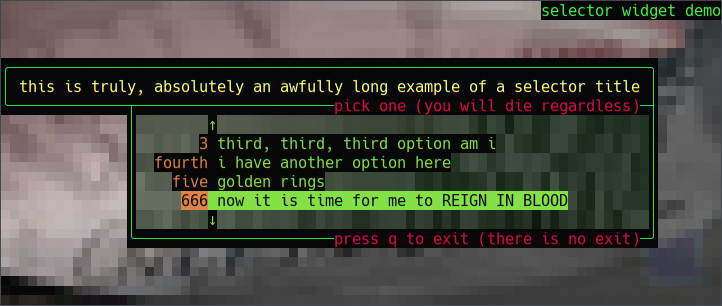
\includegraphics[width=.75\linewidth]{media/selector1.png}
    \caption{Selector with a long title.}
\end{figure}

\begin{figure}
    \centering
    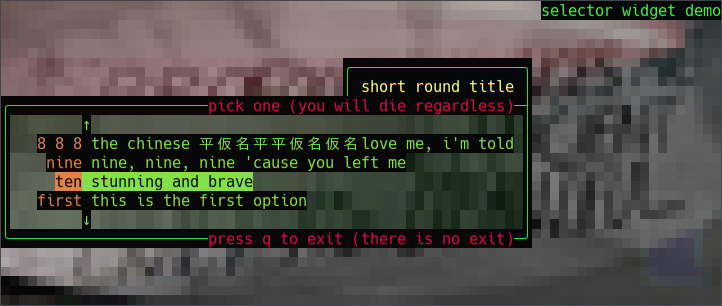
\includegraphics[width=.75\linewidth]{media/selector2.png}
    \caption{Short title intersecting with header.}
\end{figure}

\begin{figure}
  \centering 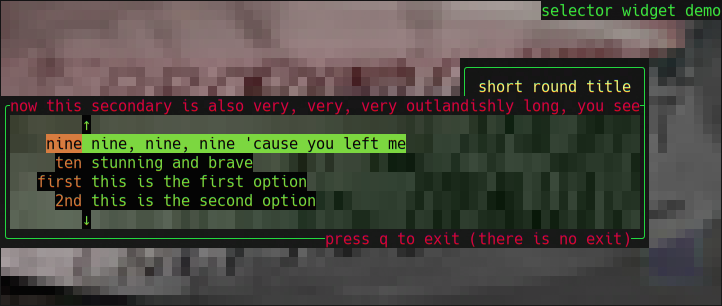
\includegraphics[width=.75\linewidth]{media/selector3.png}
    \caption{Selector with a long header.}
\end{figure}

\begin{figure}
\centering 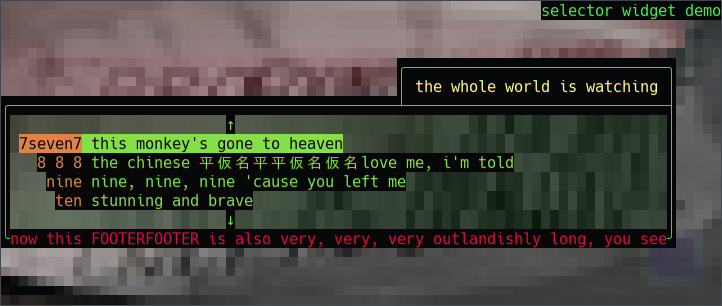
\includegraphics[width=.75\linewidth]{media/selector4.png}
\caption{Selector with a long footer and no header.}
\end{figure}

\begin{figure}
  \centering 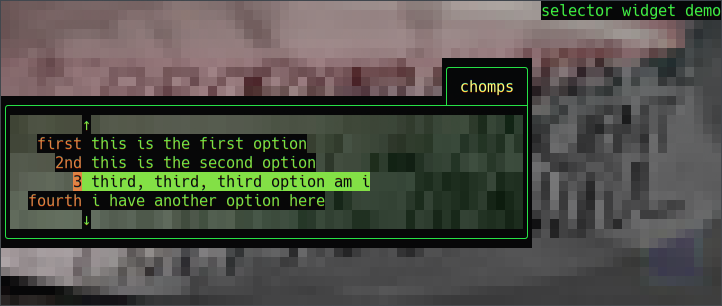
\includegraphics[width=.75\linewidth]{media/selector5.png}
  \caption{Naked selector.}
\end{figure}

\begin{listing}[!htbp]
\begin{minted}{C}
int ncselector_additem(struct ncselector* n, const struct selector_item* item);
int ncselector_delitem(struct ncselector* n, const char* item);

// Return a reference to the selected option, or NULL if there are no items.
const char* ncselector_selected(const struct ncselector* n);

// Return a reference to the ncselector's underlying ncplane.
struct ncplane* ncselector_plane(struct ncselector* n);

// Move up or down in the list. A reference to the newly-selected item is
// returned, or NULL if there are no items in the list.
const char* ncselector_previtem(struct ncselector* n);
const char* ncselector_nextitem(struct ncselector* n);

// Offer the input to the ncselector. If it's relevant, this function returns
// true, and the input ought not be processed further. If it's irrelevant to
// the selector, false is returned. Relevant inputs include:
//  * a mouse click on an item
//  * a mouse scrollwheel event
//  * a mouse click on the scrolling arrows
//  * a mouse click outside of an unrolled menu (the menu is rolled up)
//  * up, down, pgup, or pgdown on an unrolled menu (navigates among items)
bool ncselector_offer_input(struct ncselector* n, const struct ncinput* nc);

// Destroy the ncselector. If 'item' is not NULL, the last selected option will
// be strdup()ed and assigned to '*item' (and must be free()d by the caller).
void ncselector_destroy(struct ncselector* n, char** item);
\end{minted}
\caption{Selector control.}
\end{listing}

\begin{figure}
    \centering
    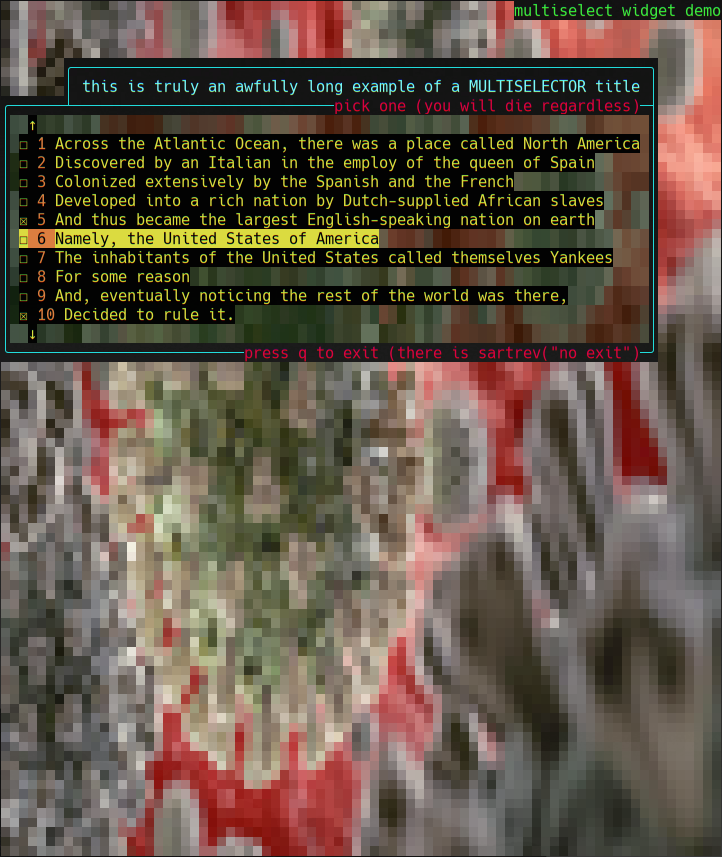
\includegraphics[width=1\linewidth]{media/multiselector.png}
    \caption{Multiselector.}
\end{figure}

\subsection{Menus}
\label{sec:menus}

Horizontal menu bars are supported on the top and bottom rows of planes. If a
menu bar is longer than the bound plane, it will be only partially visible, but
any unrolled section will be visible. Menus may be either visible or invisible
by default. Set the `hiding` option to get an invisible menu. In the event of a
screen resize, menus will be automatically moved/resized.

\begin{listing}[!htbp]
\begin{minted}{C}
typedef struct menu_options {
  bool bottom;              // on the bottom row, as opposed to top row
  bool hiding;              // hide the menu when not being used
  struct {
    char* name;             // utf-8 c string
    struct {
      char* desc;           // utf-8 menu item, NULL for horizontal separator
      ncinput shortcut;     // shortcut, all should be distinct
    }* items;
    int itemcount;
  }* sections;              // array of menu sections
  int sectioncount;         // must be positive
  uint64_t headerchannels;  // styling for header
  uint64_t sectionchannels; // styling for sections
} menu_options;

struct ncmenu;

// Create a menu with the specified options. Menus are currently bound to an
// overall notcurses object (as opposed to a particular plane), and are
// implemented as ncplanes kept atop other ncplanes.
struct ncmenu* ncmenu_create(struct notcurses* nc, const menu_options* opts);
\end{minted}
\caption{Menu creation.}
\end{listing}

\begin{figure}
    \centering
    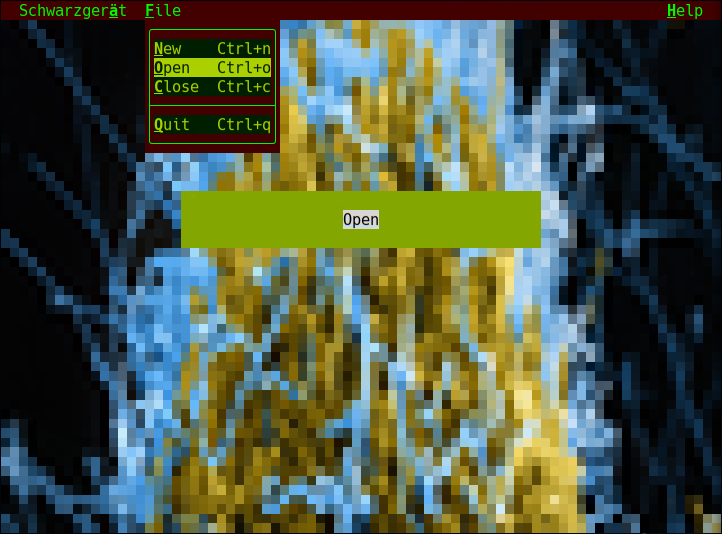
\includegraphics[width=.75\linewidth]{media/menutop.png}
    \caption{Menu along the top of the standard plane.}
\end{figure}

\begin{figure}
    \centering
    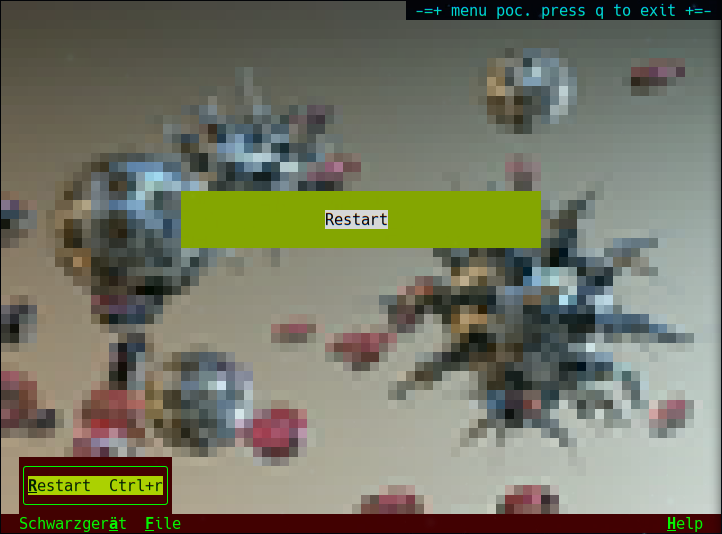
\includegraphics[width=.75\linewidth]{media/menubottom.png}
    \caption{Menu along the bottom of the standard plane.}
\end{figure}

\begin{figure}
    \centering
    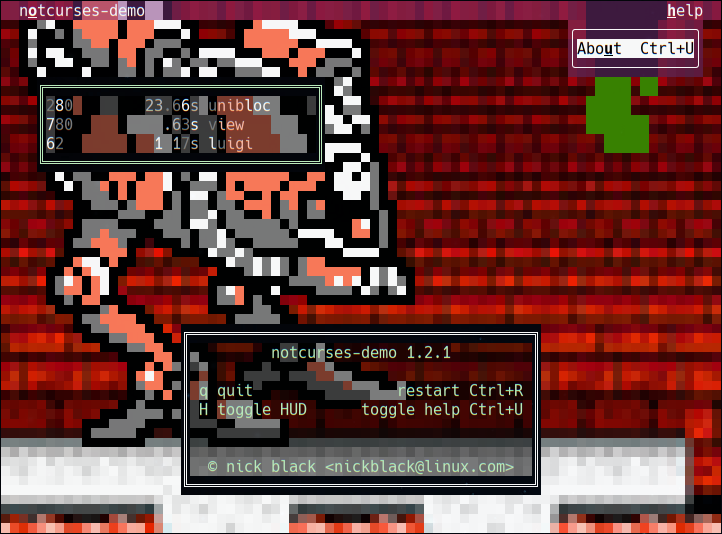
\includegraphics[width=.75\linewidth]{media/menuwarmech.png}
    \caption[WarMECH and a translucent menu.]{The \texttt{notcurses-demo} menu, unrolled \textit{in media res}. Luigi, pursued
      by WarMECH, is leaping through the ``Help'' menu. In the upper left is the HUD,
      and at the bottom the About text, both implemented as translucent planes.}
\end{figure}

\begin{listing}[!htbp]
\begin{minted}{C}
// Unroll the specified menu section, making the menu visible if it was
// invisible, and rolling up any menu section that is already unrolled.
int ncmenu_unroll(struct ncmenu* n, int sectionidx);

// Roll up any unrolled menu section, and hide the menu if using hiding.
int ncmenu_rollup(struct ncmenu* n);

// Return the selected item description, or NULL if no section is unrolled. If
// 'ni' is not NULL, and the selected item has a shortcut, 'ni' will be filled
// in with that shortcut--this can allow faster matching.
const char* ncmenu_selected(const struct ncmenu* n, struct ncinput* ni);

// Return the ncplane backing this ncmenu.
struct ncplane* ncmenu_plane(struct ncmenu* n);

// Offer the input to the ncmenu. If it's relevant, this function returns true,
// and the input ought not be processed further. If it's irrelevant to the
// menu, false is returned. Relevant inputs include:
//  * mouse movement over a hidden menu
//  * a mouse click on a menu section (the section is unrolled)
//  * a mouse click outside of an unrolled menu (the menu is rolled up)
//  * left or right on an unrolled menu (navigates among sections)
//  * up or down on an unrolled menu (navigates among items)
//  * escape on an unrolled menu (the menu is rolled up)
bool ncmenu_offer_input(struct ncmenu* n, const struct ncinput* nc);

// Destroy a menu created with ncmenu_create().
int ncmenu_destroy(struct ncmenu* n);
\end{minted}
\caption{Menu control.}
\end{listing}

\subsection{Reels}
\subsection{Example: let's rip off \texttt{whiptail}}

\section{Complex examples}
\subsection{Example: let's rip off tetris}
\label{sec:casestudy}
\subsection{Example: walking through \texttt{notcurses-demo}}
\label{sec:ncdemo}
The \texttt{notcurses-demo} program is built as part of Notcurses, and ought
have been installed alongside the library (on Debian, you'll need the
\texttt{notcurses-bin} package, and even then the demo has been somewhat
reduced in order to comply with the DFSG\cite{dfsg}). It demonstrates a wide
range of Notcurses capabilities, and its source code is most instructive.

It is best to run the demo in a terminal having geometry of at least 80x45,
though anything 80x24 or larger will more or less work (some content will be
clipped). It is also desirable to have 24-bit color enabled, assuming your
terminal supports it. Determine the number of colors advertised by your
terminal type using~\texttt{infocmp} (see Figure~\ref{fig:terminfocmp}).
Some relevant terminfo capabilities are described in Table~\ref{table:terminfo}.

\begin{table}[h]
  \begin{center}
    \begin{tabular}{ |c|c|c| }
      \hline
      \texttt{colors} & Integer & Number of colors. \\
      \hline
      \texttt{ccc} & Boolean & The palette can be programmed. \\
      \hline
      \texttt{RGB} & Boolean & Direct RGB values can be speficied. \\
      \hline
    \end{tabular}
  \end{center}
  \caption{Relevant terminfo properties.}
  \label{table:terminfo}
\end{table}

Each demo makes use of a few different Notcurses capabilities. In addition,
a menu is present throughout. From this menu (or using keyboard shortcuts),
you can activate a HUD (H) and an informational help display (Ctrl+u). In
addition, you can restart the demo with Ctrl+R, or quit at any time (q). This
application serves admirably for benchmarking certain terminal behaviors, and
we'll do exactly that in Appendix~\ref{sec:termshade}. The performance
properties of various components are described at length therein.

\begin{figure}[h]
  \centering
  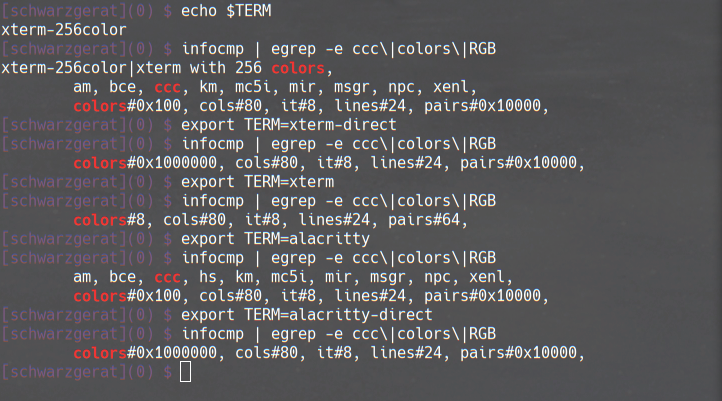
\includegraphics[width=.75\linewidth]{media/terminfocmp.png}
  \caption{Inspecting the terminfo database.}
  \label{fig:terminfocmp}
\end{figure}

Screenshots were taken using \texttt{scrot} 1.2 and a 80x45
\texttt{xfce4-terminal} 0.8.9.1 from Xfce 4.14+Compiz 0.8.16.1 atop Xorg
1.20.7 on NVIDIA 440.59. All of these are the unmodified Debian Unstable
x86\_64 binaries. My kernel is a custom 5.5.6 build. The terminal type is
\texttt{xterm-256color}, and \texttt{COLORTERM} is defined to be
\texttt{24bit}. The terminal font was Hack 10, and the background is a 0.7
transparency.

\newpage

\begin{figure}
  \centering
  \begin{minipage}{0.45\textwidth}
    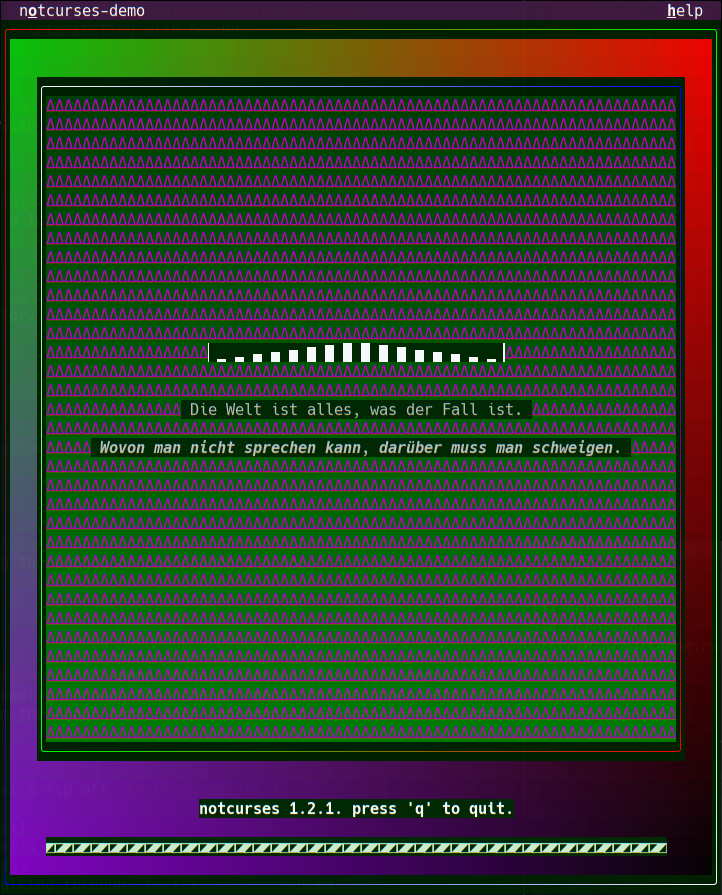
\includegraphics[width=1\linewidth]{media/demo-intro.png}
    \caption[``Intro''.]{``Intro''. Lerps on the perimeters. Inverse radial
            gradient plus vertical gradient. Full-screen fade.
            Cyclic glyphs. Italics.}
  \end{minipage}\hfill
  \begin{minipage}{0.45\textwidth}
    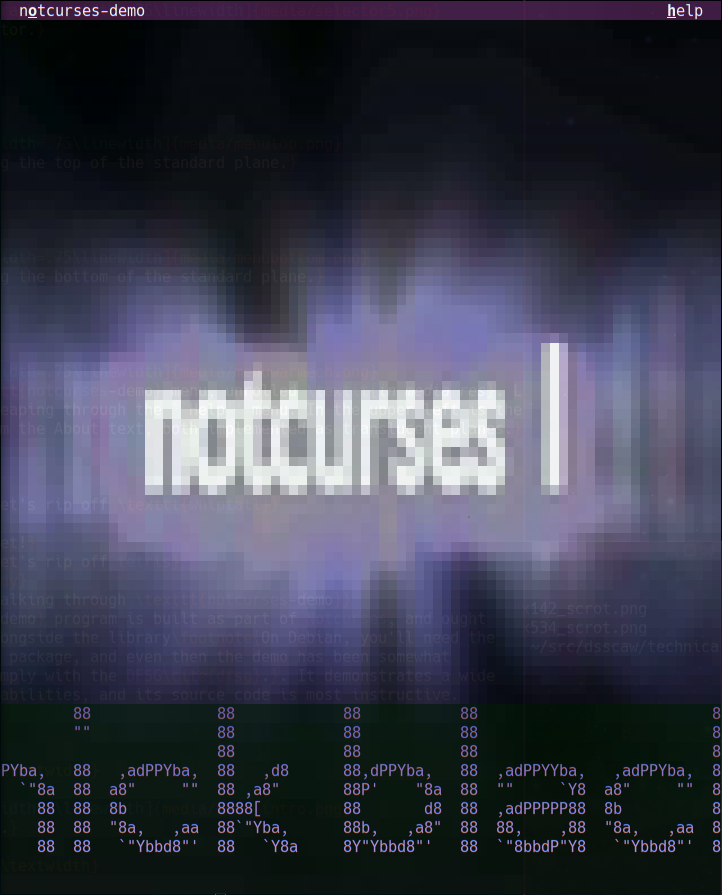
\includegraphics[width=1\linewidth]{media/demo-xray.png}
    \caption[``X-Ray''. Very large planes.]{``X-Ray''. Streaming video.
       Very large planes (the scrolling plane at the bottom is much larger than the visible screen).}
  \end{minipage}
\end{figure}

\begin{figure}
  \centering
  \begin{minipage}{0.45\textwidth}
    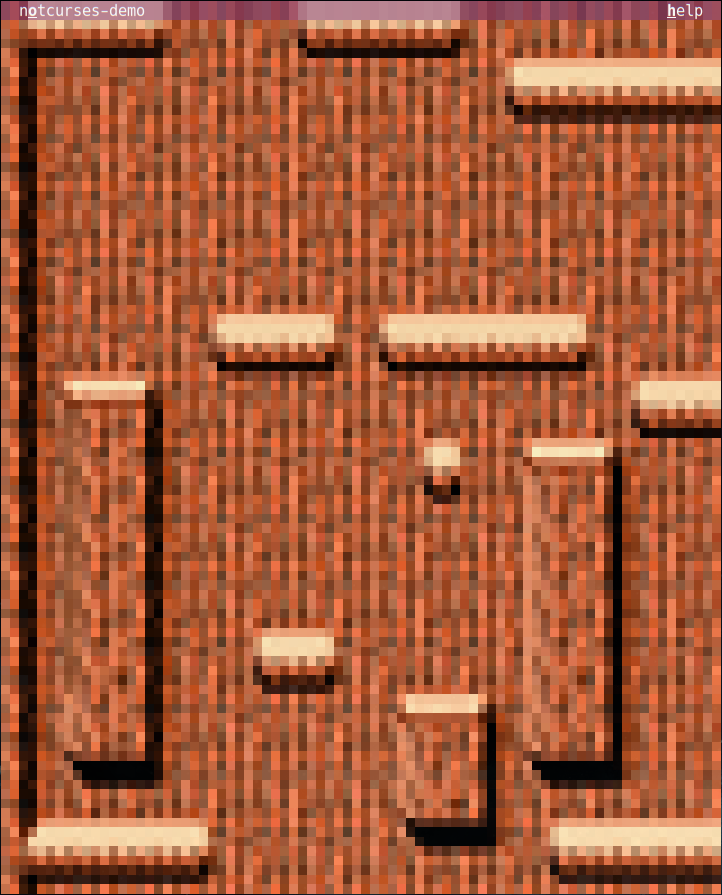
\includegraphics[width=1\linewidth]{media/demoeagle2.png}
    \caption{``Eagle'', first phase.\\
      Parallax scrolling on large image.}
  \end{minipage}\hfill
  \begin{minipage}{0.45\textwidth}
    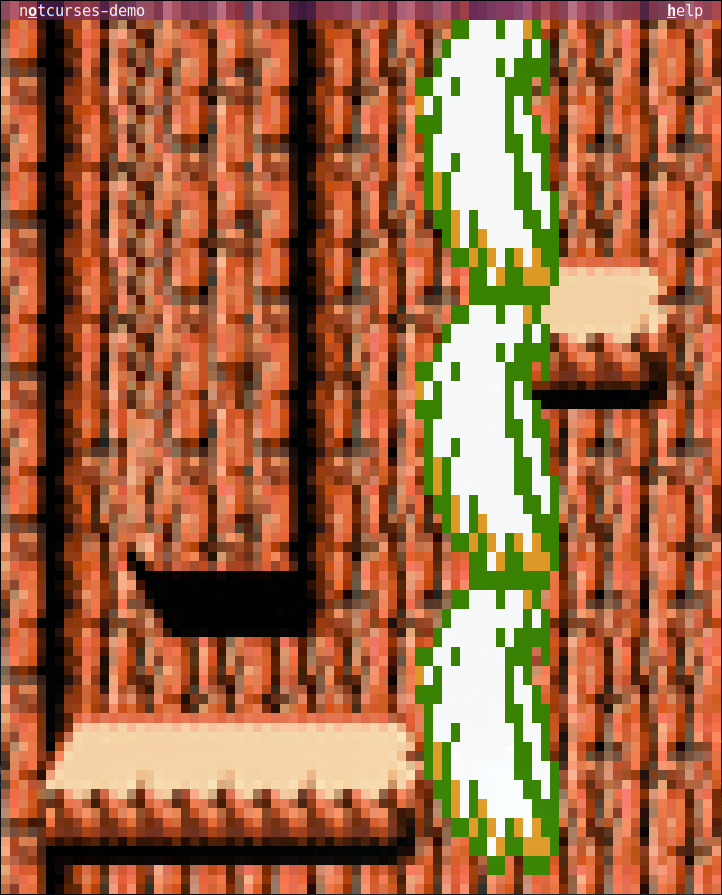
\includegraphics[width=1\linewidth]{media/demoeagle1.png}
    \caption{``Eagle'', second phase.\\
      Sprites. Zoomed image.}
  \end{minipage}
\end{figure}

\begin{figure}
  \centering
  \begin{minipage}{0.30\textwidth}
    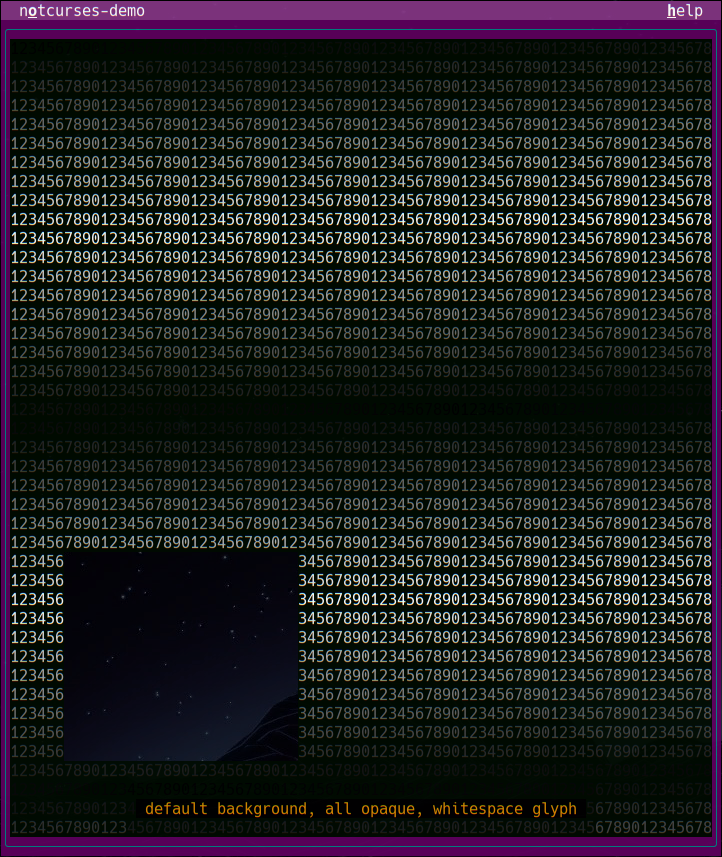
\includegraphics[width=1\linewidth]{media/demo-trans1.png}
    \caption[``Trans'', early phase.]{``Trans''. Transparent top plane. Window through to the desktop.}
  \end{minipage}\hfill
  \begin{minipage}{0.30\textwidth}
    \includegraphics[width=1\linewidth]{media/demo-trans2.png}
    \caption[``Trans'', middle phase.]{``Trans''. Opaque foreground, transparent background, no glyph.}
  \end{minipage}\hfill
  \begin{minipage}{0.30\textwidth}
    \includegraphics[width=1\linewidth]{media/demo-trans3.png}
    \caption[``Trans'', late phase.]{``Trans''. Transparent foreground and background with opaque glyph.}
  \end{minipage}\hfill
\end{figure}

\begin{figure}
  \centering
  \begin{minipage}{0.45\textwidth}
    \includegraphics[width=1\linewidth]{media/demo-highcon.png}
    \caption{``Highcon''. High-contrast text.}
  \end{minipage}\hfill
  \begin{minipage}{0.45\textwidth}
    \includegraphics[width=1\linewidth]{media/demo-grid.png}
    \caption{``Grid''. Max RGB density.}
  \end{minipage}\hfill
\end{figure}

\begin{figure}
  \centering
  \begin{minipage}{0.45\textwidth}
    \includegraphics[width=1\linewidth]{media/demo-box.png}
    \caption{``Box''. Lerped perimeters. Precise Unicode. Color sweeps.}
  \end{minipage}\hfill
  \begin{minipage}{0.45\textwidth}
    \includegraphics[width=1\linewidth]{media/demo-sliders.png}
    \caption{``Sliders''. Partial fades. Animation. Gradients.}
  \end{minipage}\hfill
\end{figure}

\begin{figure}
  \centering
  \begin{minipage}{0.45\textwidth}
    \includegraphics[width=1\linewidth]{media/demo-reels.png}
    \caption{``Reels''. The \texttt{ncreel} widget.}
  \end{minipage}\hfill
  \begin{minipage}{0.45\textwidth}
    \includegraphics[width=1\linewidth]{media/demo-whiteout.png}
    \caption{``Whiteout''. Translucency.}
  \end{minipage}\hfill
\end{figure}

\begin{figure}
  \centering \includegraphics[width=.75\linewidth]{media/demo-chunli1.png}
  \caption{``Chunli''. Sprite animation.}
\end{figure}

\begin{figure}
  \centering \includegraphics[width=.75\linewidth]{media/demo-chunli2.png}
  \caption{``Chunli''. Sprite animation.}
\end{figure}

\begin{figure}
  \centering
  \begin{minipage}{0.45\textwidth}
    \includegraphics[width=1\linewidth]{media/demo-uniblock1.png}
    \caption{``Uniblock''. Hangul syllables.}
  \end{minipage}\hfill
  \begin{minipage}{0.45\textwidth}
    \includegraphics[width=1\linewidth]{media/demo-uniblock2.png}
    \caption{``Uniblock''. Emoji.}
  \end{minipage}\hfill
\end{figure}

\begin{figure}
  \centering
  \begin{minipage}{0.45\textwidth}
    \includegraphics[width=1\linewidth]{media/demo-img1.png}
    \caption{``View''. Scaling an image.}
  \end{minipage}\hfill
  \begin{minipage}{0.45\textwidth}
    \includegraphics[width=1\linewidth]{media/demo-img2.png}
    \caption{``View''. Transparent images.}
  \end{minipage}\hfill
\end{figure}

\begin{figure}
  \centering
  \begin{minipage}{0.45\textwidth}
    \includegraphics[width=1\linewidth]{media/demo-view1.png}
    \caption{``View''. Streaming video with high-contrast text.}
  \end{minipage}\hfill
  \begin{minipage}{0.45\textwidth}
    \includegraphics[width=1\linewidth]{media/demo-view2.png}
    \caption{``View''. Notice the high-contrast kicking in.}
  \end{minipage}\hfill
\end{figure}

\begin{figure}
  \centering \includegraphics[width=1\linewidth]{media/demojungle.png}
  \caption[``Jungle''. Palette-indexed image.]{``Jungle''. Palette-indexed image. Very low-bandwidth animation via palette cycling.\\
    ``Ruins in Rain'' © Mark Ferrari/Living Worlds. Texelized with permission.}
\end{figure}


\begin{figure}
  \centering
  \begin{minipage}{0.45\textwidth}
    \includegraphics[width=1\linewidth]{media/demo-fallin1.png}
    \caption[``Fallin\''', early phase.]{``Fallin\'''. Color change, introspection, many planes.}
  \end{minipage}\hfill
  \begin{minipage}{0.45\textwidth}
    \includegraphics[width=1\linewidth]{media/demo-fallin2.png}
    \caption[``Fallin\''', late phase.]{``Fallin\'''. The underlying image is revealed.}
  \end{minipage}\hfill
\end{figure}

\begin{figure}
  \centering
  \begin{minipage}{0.45\textwidth}
    \includegraphics[width=1\linewidth]{media/demo-luigi.png}
    \caption{``Luigi''. Multiple sprites.}
  \end{minipage}\hfill
  \begin{minipage}{0.45\textwidth}
    \includegraphics[width=1\linewidth]{media/demo-outro.png}
    \caption{``Outro''. Fades atop video.}
  \end{minipage}\hfill
\end{figure}

\clearpage
\newpage
%%%%%%%%%%%%%%%%%%%%%%%%%%%%%%%%%%%%%%%%%%%%%%%%%%%%%%%%%%%%%%%%%%%%%%%%
\begin{appendices}

\section{A brief history of character graphics}
\label{sec:terminals}
The earliest terminals making use of glyphs\footnote{Konrad Zuse's Z3, generally
 considered the first programmable digital computer, communicated with its
operator through a matrix of blinkenlights and a not unsteampunkish keyboard that resembled the
Burroughs typewriters of its era\cite{zuse}.} printed them to paper, and are of
interest to us only so far as our modern term ``tty'' is rather dubiously
derived from ``TeleTYpewriter'', as these cantankerous contraptions were
known\footnote{Though we do hear of their Snoopy calendars in the songs of
legend\cite{quiche}.} (people had less experience abbreviating in those days).

These devices most typically printed 72 characters per line (CPL), a limit that
has persisted in strange places\cite{pandoc} through the modern era. Another constant
you'll see from time to time is 132 CPL, derived from line printers such as the
IBM 1403, the DEC LP11, and the Centronics 101\cite{ibm1403}. Most common,
however, is the 80 column line originating in 1928's 7¾x3¼x0.007in IBM
Computer Card (as designed by Clair D.\ Lake, deriving from the 1890 U.\ S.\
Census cards of Herman Hollerith\ldots themselves borrowing from Joseph
Jacquard's automation in 1804 of punched card loom control technology pioneered
by Basile Bouchon in 1725\cite{cards}). To this day, so long as your wacky
output device can do 80 columns, eh, that's good enough. In all these cases,
the limit arises from the number of characters that could be printed, using the
technology of the time, on their feeder paper (8.5in and 14in in the case of
printers).

On, then, to the ``Glass TTYs'' (ugh) and Visual Display Units of the 1970s.
Pictured in Figure~\ref{fig:terminals} are the Computer Terminal Corporation
Datapoint 3300, the Lear Sigler, Inc.\ ADM-3A, the Hazeltine 1500, and the
Soroc IQ-120. Lacking microcontrollers, and generally implementing no
independent control sequences, such devices are today often known as ``dumb
terminals'' (this term was originally a registered trademark of Lear Sigler,
see Figure~\ref{fig:adm3}). Already the 80x24 ``standard'' (it is not a standard) was emerging
(the DEC contemporaries listed were already pretty ``smart'', using proprietary
control codes):

\begin{table}[h]
\begin{center}
  \begin{tabular}{ |c|c|c| }
    \hline
    IBM 2260 Model 1 & 1965 & 40x6 \\
    \hline
    Datapoint 3300 & 1969 & 72x25 \\
    \hline
    DEC VT05 & 1970 & 72x24 \\
    \hline
    IBM 3277 Model 2 & 1971 & 80x24 \\
    \hline
    Textronix 4010 & 1972 & 74x35 \\
    \hline
    DECscope VT52 & 1974 & 80x24 \\
    \hline
    LSI ADM-3A & 1976 & 80x12, 80x24 \\
    \hline
    Hazeltine 1500 & 1977 & 80x24 \\
    \hline
    Sororc IQ-120 & 1977 & 80x24 \\
    \hline
  \end{tabular}
\caption{Some historical terminals and their resolutions.}
\end{center}
\end{table}

Why 80x24 (or 80x25, as you'll also see)\cite{infoworld80}? The 80 almost certainly arises from
the desire to display an entire punched card (this \textit{is} a standard---see
ANSI X3.21-1967/FIPS PUB 13, ``Rectangular Holes in Twelve-Row Punched
Cards'')\cite{sonicdelay}. The origin of 24 is less clear. 24 is highly
composite (it has more divisors than any smaller number), and it is the largest
integer divisible by all natural numbers not larger than its square root. There
are of course 24 hours in a day. 24 divides the scanline counts of both NTSC
and PAL at 480 and 576, respectively. 24 rows of 80 columns at a byte per
column utilize 93.75\% of a 2KiB memory, leaving exactly 128 bytes left over,
and everyone loves a good power of 2.

The Aaronites, Levite descendents of Moses's brother Aaron, the first
\texthebrew{כהן גדול}
(High Priest),
form the priestly \texthebrew{כֹּהֲנִים}; they were divided into 24 courses. The Buddha's Dharma Chakra (Wheel of Dhamma)
in its Ashoka form sends forth 24 spokes. But perhaps I grow esoteric, even
speculative\ldots in truth, 80x24 almost certainly owes its questionable
existence to IBM's punched cards, IBM 2260 and 3270 wanting compatibility with
IBM printers, the upstart DEC wanting compatibility with IBM software for their
VT52 and legendary VT100, and the VT100 subsequently becoming a \textit{de facto} standard for
four decades.

\begin{figure}
  \centering \includegraphics[width=.9\linewidth]{media/dumbterminals.jpg}
\caption[Dumb terminals of the 1970s.]{Clockwise starting from upper left: a dork and his LSI ADM (``American
  Dream Machine'', supposedly). That poor woman with the Sororc IQs looks stoned out
  of her gourd. Grizzly Adams rocks a Datapoint 3300, but really his mind is on
  seeing Skynyrd shred it this weekend. Finally, we have Frank the Cocaine
  Ranger and his Electric Hazeltine 1500 Band. \textit{Gott im Himmel}, the 70s were \textit{unseemly}.}
\label{fig:terminals}
\end{figure}

\begin{figure}
  \begin{minipage}{0.5\textwidth}
  \centering
    \includegraphics[width=.5\linewidth]{media/digital-terms.jpeg}
    \caption{Digital Equipment Corporation terminals of the 1970s and 1980s.}
  \end{minipage}\hfill
  \begin{minipage}{0.4\textwidth}
  \centering
    \includegraphics[width=.45\linewidth]{media/vt220-charset.png}
    \caption[VT220 glyph dump.]{The VT220's glyphs from a ROM dump. VT100 implemented most of the
      first seven columns. Note the existence of box-drawing characters\cite{crttypography}.}
  \end{minipage}\hfill
\end{figure}

\begin{figure}
  \centering
  \includegraphics[width=.8\linewidth]{media/adm3.jpeg}
  \caption{A strange time.}
  \label{fig:adm3}
\end{figure}

\subsection{The DEC VTxxx terminals and ANSI X3.64-1979}

Introduced in August 1978, the VT100 ushered in a new era of smart terminals
using commodity (Intel) microprocessors, implementing portions of the upcoming
ANSI X3.64 standard (itself based on 1976's first edition of ECMA-48) along
with DEC extensions\footnote{The VT100 \textit{did not} implement all of X3.64,
nor was X3.64 derived from the VT100. The VT100 didn't do color, nor did it
insert or delete lines. It furthermore implemented several features outside
the scope of ECMA-48's first edition.} This series would go on to sell over
six million units, and it was a rare vendor that didn't include some degree
of DEC VT compatibility. Each major iteration of the series was designed to
encompass all functionality of prior iterations, beginning with the VT100's
faithful emulation of the earlier era's VT52\cite{vt52}. The VT102 cut down on the cost
and size of the VT100, and included the 132-CPL mode by default; they were
otherwise essentially the same device\cite{vt100}.

Terminals had quite a heyday through the 1970s and 1980s, but as the price of
Wintel machines fell below \$1,000, their purpose rapidly eroded. They lived on,
especially in niche minicomputer and mainframe installations, but as of 2020 it's
difficult to find a new terminal. Digital sold their terminal business to SunRiver
Data Systems (now Boundless Technologies) in 1995; the \url{boundlessterminals.com}
site is not offered over HTTPS, and reads ``Now it is time for the last text
terminals to give way to newer technologies\cite{boundless}.'' Press F to pay
respects.

The original \texttt{xterm} (released in X10R3) was written as an emulator of
the VAXStation 100 (VS100), and slowly acquired scattered features from the
VT100, ANSI, and other sources\cite{xtermfaq}. Thomas E.\ Dickey (the current
maintainer of \Gls{ncurses} and xterm) began working on XTerm in the mid-90s,
and by 1996 had added the \texttt{decTerminalID} resource following the
addition of much VT220 compatibility. \texttt{xterm} can be built with support
for Sixel, ReGIS, Unicode, and an extraordinary number of archaic and/or
baroque mechanics with which I'm not personally familiar. Further information
is available in Mr.\ Dickey's
\href{https://invisible-island.net/xterm/xterm.faq.html}{XTerm FAQ}, which
makes for excellent reading\footnote{Mr. Dickey's XTerm and NCURSES FAQs are,
in my opinion, two of the finest pieces of technical documentation in
existence. It is my hope that this manuscript approaches their level.}.

I will not attempt to list the hundreds (probably thousands) of terminal
emulators that are available. Most claim some manner of ``ANSI'' or ``vt100''
(not the same thing!) compliance; take these claims with a large grain of salt.
It's worth knowing about:

\begin{denseitemize}
\item{\texttt{rxvt}, ``Rob's \texttt{xvt}''. An enhancement of \texttt{xvt} touted
    as a slimmed-down, simplified alternative to \texttt{xterm}. Implemented pixel-addressable
    graphics (in a scheme incompatible with Sixel). Like \texttt{xterm}, it uses
    X resources for configuration. Various forks add various essential technologies
    introduced since 2000.}
\item{Konsole, the official terminal of KDE. Having never used KDE substantially,
   I've never made much use of Konsole. I recall it having URL recognition
   when most terminal emulators didn't.}
\item{VTE terminals, a family of terminals built around GNOME's VTE library, built
  atop GTK3. GNOME and Xfce's terminals both wrap VTE, as do dozens of others.
  \texttt{xfce4-terminal} plays the role of our VTE terminal in benchmarks, because
  I run XFCE (atop Compiz).}
\item{\texttt{alacritty}, written in Rust by Joe Wilm. One of the new class of
    emulators written directly against OpenGL.}
\item{\texttt{kitty}, another OpenGL program, this one in Python by Kovid Goyal.}
\item{Terminology is the emulator of Enlightenment since E17, the long (twelve
    years!) awaited successor to E16. It seemed somewhat broken every time I
    tried it, and by 2014 I didn't want to spend time fixing terminal emulators.
    It does look really pretty on its website\cite{terminology}.}
\item{Terminator was written in Java, which\textellipsis life finds a way I guess.}
\end{denseitemize}

I haven't benchmarked \texttt{rxvt} because I didn't care to figure out which of
its ten thousand forks is the one you're supposed to use. Likewise, I didn't
benchmark Terminator because I would legitimately prefer setting myself on fire
to running a Java terminal emulator.

The best single source of terminal emulator (and terminal) information is
probably the ``Terminal Type Descriptions'' file distributed with NCURSES\cite{termdescript}.

\subsection{The Curses API}
Several APIs for TUIs and character (semi)graphics have emerged over the fifty
years of video terminals' existence. Of them, by far the most venerable,
portable, and proven is Curses, which has (for over twenty years) actually
been codified in the Single UNIX Specification. Notcurses is an obvious
intellectual descendant of Curses, and indeed ought be easy to pick up by any
experienced Curses programmer.

As mentioned in Chapter ~\ref{sec:terminfo}, Ken Arnold released the first BSD
Curses library shortly after extracting \texttt{vi}'s terminal abstraction routines
as libtermcap, and that first Curses made use of termcap\cite{cursesexplained}.
Similarly to termcap, Curses had its origins in Joy's \texttt{vi} code; unlike
termcap, Curses required significant reworking to be presented as a sensible
API. Meanwhile, over in AT\&T land, Mary Ann Horton (previously maintainer of
BSD's \texttt{vi} and \texttt{termcap}) arrived and implemented a new Curses,
this one making use of her terminfo. The two diverged over the years (with PDCurses
aka Public Domain Curses reimplementing AT\&T to work around licensing issues),
until X/Open codified an official vendor-neutral Curses, publishing it in
1996's Issue 4, version 2 (this specification derived primarily from SVR4 Curses).

Zeyd Ben-Halim adapted ncurses from the pcurses project of Pavel Curtis. Dickey
reports the 1.8.1 version released 1993-11-05 (and included with Slackware 2.0.1)
as the ``first widely-used version''. Numerous people (including the notorious
Eric S. Raymond and Ulrich Drepper) contributed significant code, but most NCURSES
development in recent years has been the work of Thomas Dickey.

The Curses API is best reviewed by reading the comprehensive man pages installed
with NCURSES. A few lines follow, summarizing major differences between Curses and Notcurses:

\begin{denseitemize}
\item{Curses has no built-in concept of a z-axis without use of its Panels
    extension, and its \texttt{stdscr} (analogous to the standard plane of
    Notcurses) is not considered part of the Panels stack. Curses does, however,
    allow windows to share memory, a capability Notcurses does not yet offer.}
\item{Panels can be ``hidden'', i.e.\ removed from the z-axis entirely. This cannot
    be done in Notcurses (but planes can be hidden underneath an opaque plane).}
\item{NCURSES defines its color API in terms of ``color pairs''. It is true that some
    terminals require both colors to be changed at the same time, but Notcurses
    hides this fact from the programmer, and instead allows foregrounds and backgrounds
    to be specified wholly independently.}
\item{Curses does not include the Panel, Menu, or Form extensions distributed
    with NCURSES. With that said, their presence in NCURSES effectively means
    they're in Curses. Notcurses is built around a Panel-like concept, and
    includes menus in its base, but lacks the rich Forms capabilities of NCURSES.}
\item{NCURSES supports only up to 256 colors at a time, as components of up to
    32,767 color pairs. There are no such limits in Notcurses (assuming terminal support).}
\item{NCURSES considers it an error to move a window or cursor off the screen. This
    is not an error in Notcurses.}
\end{denseitemize}

\pagebreak
\newpage

\newpage
%%%%%%%%%%%%%%%%%%%%%%%%%%%%%%%%%%%%%%%%%%%%%%%%%%%%%%%%%%%%%%%%%%%
\section{Wherein shade is thrown at current terminal emulators}
\label{sec:termshade}
\textbf{FIXME FIXME FIXME}
graphs i want:
\begin{denseitemize}
\item{emulator performance as a function of size}
\item{emulator performance as a function of bandwidth--same color everywhere, but turn off elision}
\item{emulator performance as a function of color change--difference with color restored relative to previous}
\item{emulator performance as a function of glyph variation}
\item{some basic perf flame graphs}
\end{denseitemize}
\newpage
%%%%%%%%%%%%%%%%%%%%%%%%%%%%%%%%%%%%%%%%%%%%%%%%%%%%%%%%%%%%%%%%%%%

\section{The Linux console}
The Linux console\footnote{The FreeBSD console is its own bag of wonders.} is
substantially different from the X and Wayland terminal emulators to which one
might be more accustomed\footnote{Muddying the issue is the fact that video
backends are sometimes described as consoles. The ``Linux console'' is a terminal
emulator running atop some video backend---on the x86, typically either VGA
Text Mode, or some trivial renderer atop a graphics-mode framebuffer
(e.\ g.\ EFIfb or vesafb.)}. Modern terminal emulators are generally more capable
than the Linux console in several ways:

\begin{denseitemize}
\item{While the Linux console accepts RGB specifiers, it downsamples them to
    far fewer colors.}
\item{Console font capabilities are extremely limited.}
\end{denseitemize}

Like any interface to a termios\cite{termios} implementation, the \texttt{IUTF8}
flag should be set (consult \texttt{stty}). This can be accomplished with the
\texttt{IUTF8} termios flag (or \texttt{stty iutf8} on the command line). This
is necessary for the terminal to interpret your output as multibyte UTF-8. The
keyboard driver ought be placed into UTF-8 mode using the \texttt{KDSKBMODE}
ioctl; the \texttt{kbd-mode} tool does this when invoked with \texttt{-u}.
This is necessary for character erase to function properly in cooked mode. Some
keyboards generate scancodes beyond the essential 128 characters, and these
should be mapped to their UTF-8 equivalents. This can be accomplished with
\texttt{dumpkeys | loadkeys --unicode}\footnote{If you've ever seen the script
\texttt{unicode\_start}, this is exactly what it does.}. This functionality has
been supported since Linux 2.6.4, released 2004-03-11, and is almost certainly
already being done in your environment.

Ensure, as always, that \texttt{LANG} is properly set, that your program
initializes the locale with \texttt{setlocale(3)}, and that \texttt{TERM} is
properly set (in this case, to one of the ``linux*'' variants).

\textbf{FIXME FIXME FIXME talk about console font}

Consult the \textit{The Linux Programmer's Manual} for more information,
particularly
\texttt{ioctl\_console(2)}\cite{ioctlconsole},
\texttt{ioctl\_tty(2)}\cite{ioctltty},
\texttt{termios(3)}\cite{termios},
\texttt{console\_codes(4)}\cite{consolecodes},
and
\texttt{charsets(7)}\cite{charsets7}.

\newpage
%%%%%%%%%%%%%%%%%%%%%%%%%%%%%%%%%%%%%%%%%%%%%%%%%%%%%%%%%%%%%%%%%%%
\section{Unicode 13}
The Unicode Consortium has scheduled Unicode 13.0 for a March 2020 release.
Chapters 3 and most of Chapter 4 of the Core Specification are normative. The
remainder is informative. The Unicode Standard consists of the Core
Specification\cite{unicode13}, the \href{https://www.unicode.org/charts/}{code charts},
the \href{https://unicode.org/versions/Unicode13.0.0/#Unicode_Standard_Annexes_nb}{Unicode Standard Annexes},
and the \href{http://www.unicode.org/Public/13.0.0/}{Unicode Character Database (UCD)}.

A Unicode Standard Annex (UAX) forms an integral part of the Unicode Standard,
but is published online as a separate document. The Unicode Standard may
require conformance to normative content in a Unicode Standard Annex, if so
specified in the Conformance chapter of that version of the Unicode Standard.
The version number of a UAX document corresponds to the version of the Unicode
Standard of which it forms a part.

\begin{table}[h]
\begin{center}
  \begin{tabular}{ |c|c| }
    \hline
    UAX \#9 & Unicode Bidirectional Algorithm \\
    \hline
    UTS \#10 & Unicode Collation Algorithm \\
    \hline
    UAX \#11 & East Asian Width \\
    \hline
    UAX \#14 & Unicode Line Breaking Algorithm \\
    \hline
    UAX \#15 & Unicode Normalization Forms \\
    \hline
    UAX \#24 & Unicode Script Property \\
    \hline
    UAX \#29 & Unicode Text Segmentation \\
    \hline
    UAX \#31 & Unicode Identifier and Pattern Syntax \\
    \hline
    UAX \#34 & Unicode Named Character Sequences \\
    \hline
    UAX \#38 & Unicode Han Database (Unihan) \\
    \hline
    UTS \#39 & Unicode Security Mechanisms \\
    \hline
    UAX \#41 & Common References for Unicode Standard Annexes \\
    \hline
    UAX \#42 & Unicode Character Database in XML \\
    \hline
    UAX \#44 & Unicode Character Database \\
    \hline
    UAX \#45 & U-Source Ideographs \\
    \hline
    UTS \#46 & Unicode IDNA Compatibility Processing \\
    \hline
    UAX \#50 & Unicode Vertical Text Layout \\
    \hline
    UTS \#51 & Unicode Emoji \\
    \hline
  \end{tabular}
\caption{Unicode 13.0.0 Standard Annexes and Synchronized Technical Standards.}
\end{center}
\end{table}

\newpage
%%%%%%%%%%%%%%%%%%%%%%%%%%%%%%%%%%%%%%%%%%%%%%%%%%%%%%%%%%%%%%%%%%%

%\section{Notcurses header files}
%\subsection{The \texttt{notcurses.h} header}
%\bgroup
%\inputminted[linenos,breaklines=true]{C}{code/notcurses.h}
%\egroup
%
%\subsection{The \texttt{nckeys.h} header}
%\bgroup
%\inputminted[linenos,breaklines=true]{C}{code/nckeys.h}
%\egroup

\end{appendices}
\newpage
%%%%%%%%%%%%%%%%%%%%%%%%%%%%%%%%%%%%%%%%%%%%%%%%%%%%%%%%%%%%%%%%%%%%%%%%
\glsaddallunused
\printglossary[title={Glossary of terms}]
\newpage
%%%%%%%%%%%%%%%%%%%%%%%%%%%%%%%%%%%%%%%%%%%%%%%%%%%%%%%%%%%%%%%%%%%%%%%%
\addcontentsline{toc}{section}{References}
\printbibliography
%%%%%%%%%%%%%%%%%%%%%%%%%%%%%%%%%%%%%%%%%%%%%%%%%%%%%%%%%%%%%%%%%%%%%%%%
%\newpage
%\vfill
%\begin{center}
%\includegraphics[width=.4\linewidth]{../common/dsscaw-purp-scaled.png}
%\includegraphics[width=.5\linewidth]{../common/south.png}
%\end{center}
%\vfill
\end{document}
